\documentclass[12pt]{article}
\usepackage[T1]{fontenc}
\usepackage[utf8]{inputenc}
\usepackage[spanish]{babel}\decimalpoint
\usepackage{graphicx} % Para comando \includegraphics[]{}
\usepackage{tikz} %Grafico de flujos
%\usetikzlibrary{arrows}
\usepackage{amsmath}
\usepackage{amssymb} %Para usar el símbolo del conj. de los Reales.%
\usepackage{diffcoeff} %Para derivada de Leibniz en un punto x%
\usepackage{hyperref} % Siempre debe ser el último paquete.

\setlength{\parindent}{0em} %justificado%
\setlength{\parskip}{1em} %espacio entre párrafos%
\renewcommand{\baselinestretch}{1.15} %line-space%



\begin{document}

\title{Apuntes `Calculus 1A: Differentiation'}
\author{}
\date{}
\maketitle

\tableofcontents

\newpage



\section{Derivación.}

\subsection{Aproximación Lineal.}

Comencemos esta sección con el siguiente ejemplo de un bote desplazándose en un canal. Digamos que $x = x(t)$ corresponde a la posición del bote a lo largo del canal en función del tiempo $t$, en donde $t$ es medido en segundos ($seg$) y $x$ en metros ($m$). Supongamos que en $t = 20 \, seg$, sabemos que el bote está en el punto $150 \, m$ del canal y está viajando en dirección positiva ($\rightarrow$) a una velocidad de $0.4 \, m/seg$.

\begin{figure}[hbt!]
\centering
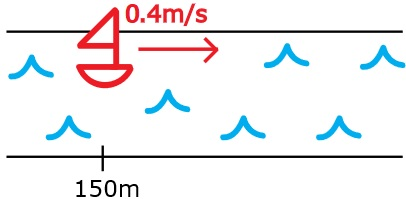
\includegraphics[scale=0.7]{img/approx_lin_examp.jpg}
\end{figure}

Como vemos, entonces, manejamos dos piezas de información:

\begin{enumerate}
\item El bote está a $x = 150 \,m$ en $t = 20 \, seg$.
\item Su velocidad es de $0.4 \, m/seg$.
\end{enumerate}

Ahora, digamos que queremos \textbf{aproximar} la posición que puede tomar el bote en $t = 30\, seg$, es decir, $10$ segundos más tarde. Una manera de pensar aquello, es \textbf{simplificando este supuesto}, asumiendo que la velocidad es la misma en estos $10 \, seg$ posteriores, en otras palabras, \textbf{la velocidad se mantiene constante en dicho período}. Y, a partir de lo que acabamos de asumir, podemos entonces multiplicar la velocidad por estos 10 segundos adicionales, bajo la ``regla de tres'':
\[\frac{0.4 \, m}{x} = \frac{1 \, seg}{10 \, seg}\]
\[x \cdot 1 \, seg = 0.4 \, m \cdot 10 \, seg\]
\[x = \frac{0.4 \, m \cdot 10 \, seg}{1 \, seg}\]
\[x = 4 \, m\]
Podemos decir, entonces, que el bote avanzó $4 \, m$ en esos $10 \, seg$ (asumiendo que la velocidad se mantiene constante), en otras palabras, corresponde a la diferencia de la posición que hay entre los $150 \,m$ y la nueva posición en $t = 30 \, seg$. Por lo tanto, \textbf{nuestra mejor apuesta o a qué posición se aproxima el bote en ese período de tiempo, será de $154 \, m$ en $t = 30 \, seg$}.

Otra forma de pensar a cuál posición se aproxima el bote en $t = 30 \, seg$, es hacerlo usando \textbf{líneas tangentes} y manejamos dos piezas de información relevantes para ello:

\begin{enumerate}
\item Conocemos un punto: P($20 \, seg$, $150 \, m$).
\item La tasa de cambio instantánea en dicho punto P: $x'(20) = 0.4 \, m/seg$, en otras palabras, la pendiente de la línea tangente.
\end{enumerate}

Dibujemos un bosquejo lo que acabamos de mencionar.

\begin{figure}[hbt!]
\centering
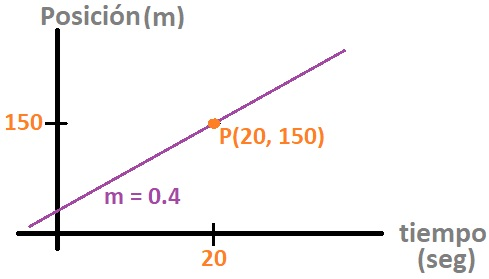
\includegraphics[scale=0.7]{img/approx_lin_examp_2.jpg}
\end{figure}

\newpage

Todo esto es lo que sabemos del gráfico, nada más. En ese sentido, éste podría verse de una o de otra forma, como lo podemos ver en la siguiente imagen:

\begin{figure}[hbt!]
\centering
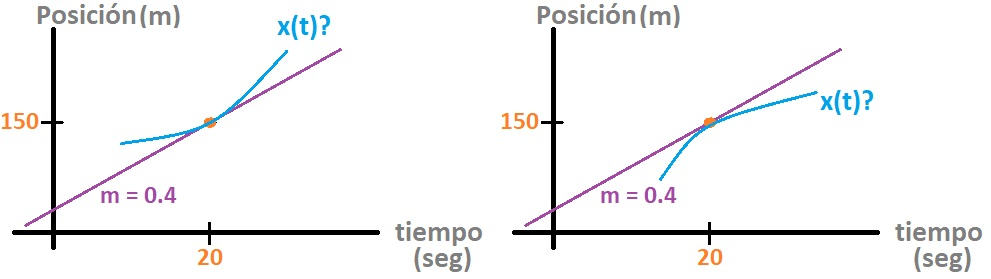
\includegraphics[scale=0.6]{img/approx_lin_examp_3.jpg}
\end{figure}

Esto, con la información que manejamos, aún no lo podemos saber con exactitud. Solo sabemos que, en el punto P($20 \, seg$, $150 \, m$), la línea tangente se ve de esa manera, con una pendiente de $0.4 \, m/s$. No obstante, nos podemos ayudar de la línea tangente para aproximar la posición del bote en $t = 30 \, seg$, porque sabemos que va a estar bastante cerca cercano al punto P($20 \, seg$, $150 \, m$).

Entonces, lo que podemos hacer es aproximar el valor de nuestra función $x(30)$, a partir de la altura de la línea tangente, en $t = 30 \, seg$, como lo podemos ver en la siguiente imagen.

\begin{figure}[hbt!]
\centering
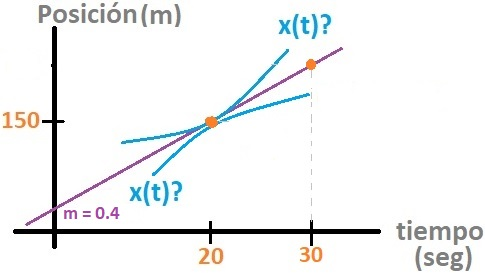
\includegraphics[scale=0.75]{img/approx_lin_examp_4.jpg}
\end{figure}

Ahora bien, ¿qué tan arriba está este nuevo punto en la línea tangente? Como hemos visto, hemos comenzado desde la altura de $150 \, m$ y, la distancia horizontal entre dicho punto y el que está en $t = 30 \, seg$, es de $10 \, seg$ ($30 \,seg - 20 \, seg$). Por otra parte, sabemos que la pendiente de la línea tangente es $m = 0.4 \, m/s$ (que es cte, también), de manera que la distancia vertical entre ambos puntos volverá a ser de $0.4 \cdot 10 = 4 \, m$, lo que quiere decir que el punto en $t = 30\, seg$ está a $150 \, m + 4 \, m = 154 \, m$. Todo esto lo podemos ver en la imagen de abajo.

\begin{figure}[hbt!]
\centering
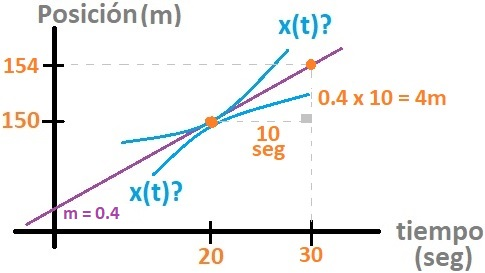
\includegraphics[scale=0.75]{img/approx_lin_examp_5.jpg}
\end{figure}

Esto mismo también lo podemos obtener usando la fórmula para calcular una pendiente. En particular, la que corresponde a la de la línea tangente, que ya sabemos que es igual a $0.4$. Simplemente, despejamos el valor de la altura en $t = 30 \, seg$:
\[m = \frac{x_{2} - x_{1}}{t_{2} - t_{1}}\]
\[0.4 \, m/seg = \frac{x_{2} - 150 \, m}{(30 - 20) \, seg}\]
\[0.4 \, m/seg = \frac{x_{2} - 150 \, m}{10 \, seg}\]
\[0.4 \, m/seg \cdot 10 \, seg = x_{2} - 150 \, m\]
\[4 \, m + 150 \, m = x_{2}\]
\[154 \, m = x_{2}\]
En definitiva, hicimos el mismo cálculo que anteriormente (págs 2-3), en donde tratamos la velocidad como constante, lo cual es similar a como \textbf{si hubiésemos asumido} en los gráficos que \textbf{la línea recta (línea tangente, en este caso) tuviera una pendiente constante}.

Lo interesante de trabajar esta aproximación a partir de \textbf{líneas tangentes} y no solo como una velocidad, es que las primeras \textbf{funcionan en muchos otros contextos, de manera tal que no necesitamos tener un movimiento físico para pensar en aquello}.

\underline{Veamos el siguiente ejemplo}: Usemos las técnicas que hemos visto hasta ahora para estimar el valor de $\sqrt{104}$ \textbf{sin calculadora}, asumiendo que podemos encontrar el valor de $\sqrt{100}$ y también la derivada de $g(x) = \sqrt{x}$ en $x = 100$.

Partamos por calcular la derivada de la función $g(x) = \sqrt{x}$.
\[\diff*{g(x)}x = \diff*{\sqrt{x}}x\]
\[\diff*{g(x)}x = \diff*{x^{1/2}}x\]
\[\diff*{g(x)}x = \frac{1}{2} (x^{1/2 - 1})\]
\[\diff*{g(x)}x = \frac{1}{2} (x^{-1/2})\]
\[\diff*{g(x)}x = \frac{1}{2} \left(\frac{1}{x^{1/2}}\right)\]
\[\diff*{g(x)}x = \frac{1}{2} \left(\frac{1}{\sqrt{x}}\right)\]
\[\diff*{g(x)}x = \frac{1}{2\sqrt{x}}\]
\[\diff*{g(x)}x = \frac{2\sqrt{x}}{4x}\]
\[\diff*{g(x)}x = \frac{\sqrt{x}}{2x}\]
Ahora calculemos la derivada de $g(x)$ en $x = 100$.
\[\diff*{g(x)}x[x = 100] = \frac{\sqrt{x}}{2x}\]
\[\diff*{g(x)}x[x = 100] = \frac{\sqrt{100}}{2 \cdot 100}\]
\[\diff*{g(x)}x[x = 100] = \frac{10}{2 \cdot 100}\]
\[\diff*{g(x)}x[x = 100] = \frac{1}{2 \cdot 10}\]
\[\diff*{g(x)}x[x = 100] = \frac{1}{2} \cdot \frac{1}{10}\]
\[\diff*{g(x)}x[x = 100] = 0.5 \cdot 0.1\]
\[\diff*{g(x)}x[x = 100] = 0.05\]
Por lo tanto, la derivada de $g(x)$ en $x = 100$, es igual $0.05$.

Justamente, como se señala en el ejemplo, podemos encontrar el valor de $\sqrt{100}$, lo cual es lo mismo que decir $g(100) = 10$. Por lo tanto, grafiquemos el punto ($100$, $10$), así como su línea tangente, cuya pendiente es $g'(100) = 0.05$.

\begin{figure}[hbt!]
\centering
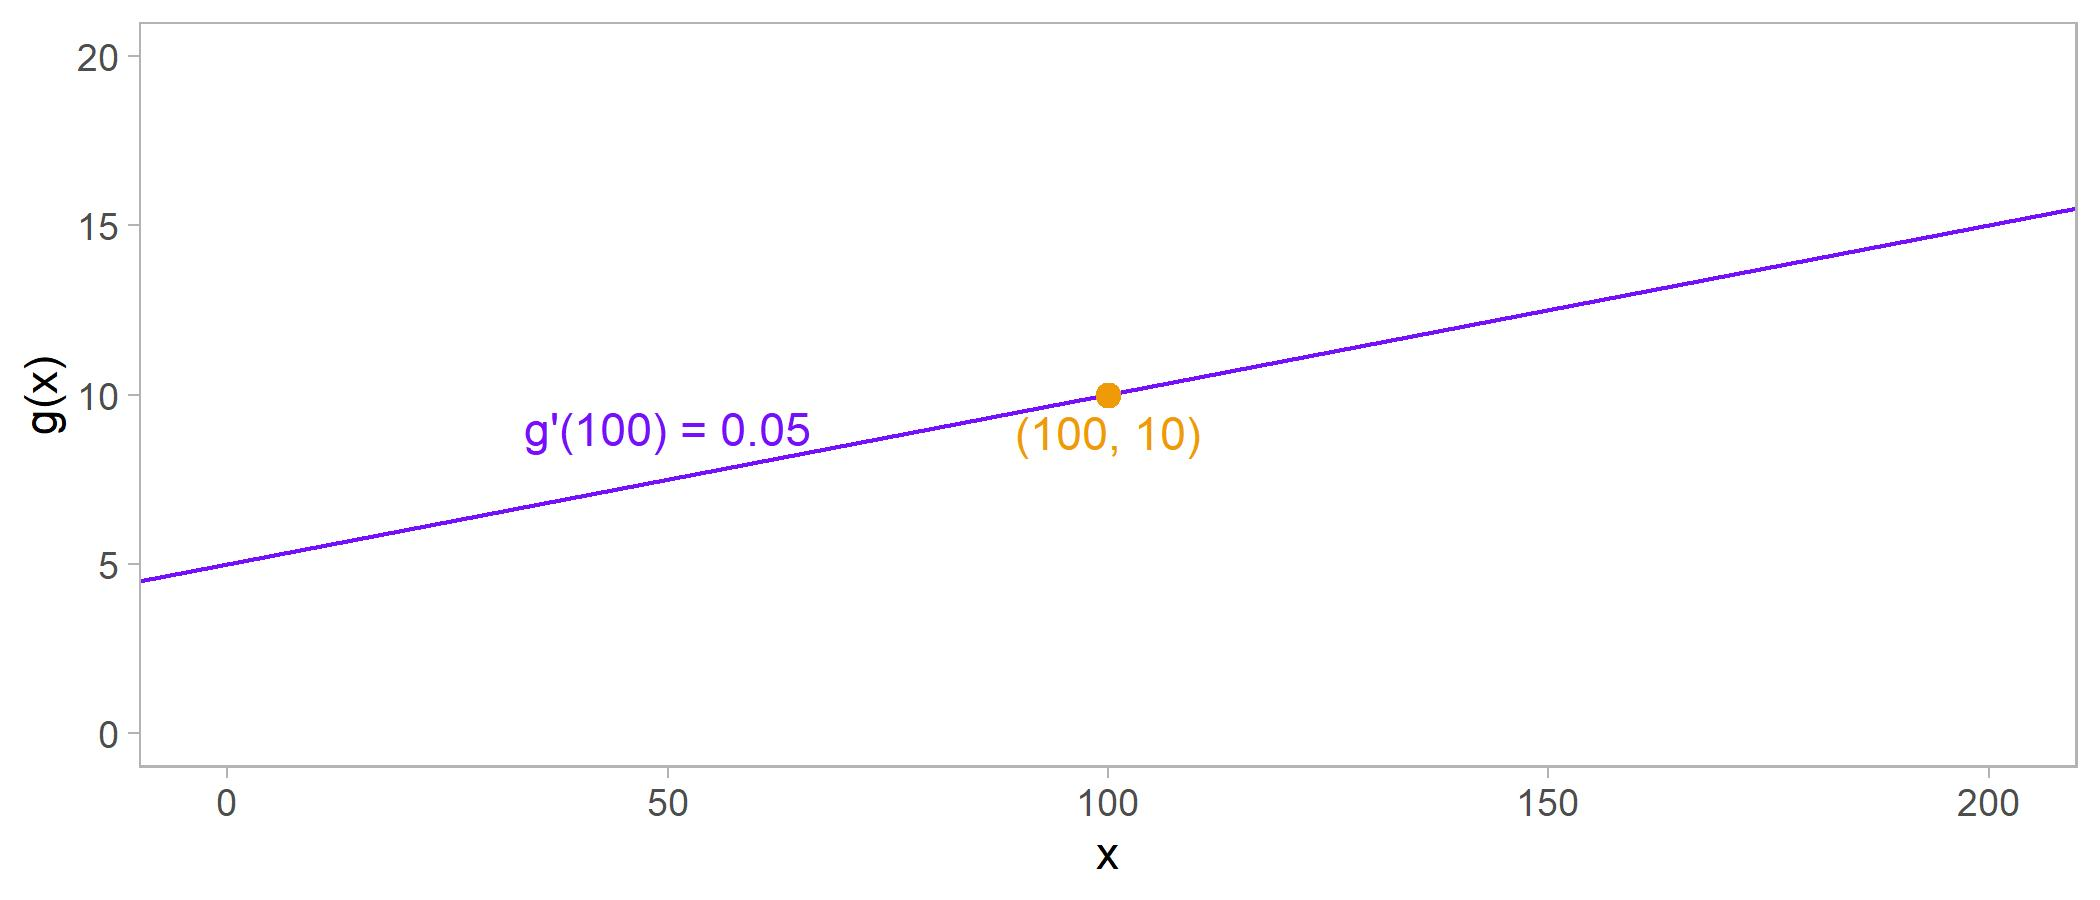
\includegraphics[scale=0.7]{img/approx_lin_sqrt.jpg}
\end{figure}

Ahora bien, nuestro objetivo es saber cuál es el valor de $g(x)$ en $x = 104$ o, en otras palabras, la $\sqrt{104}$, sin hacer uso de una calculadora.

\newpage

\begin{figure}[hbt!]
\centering
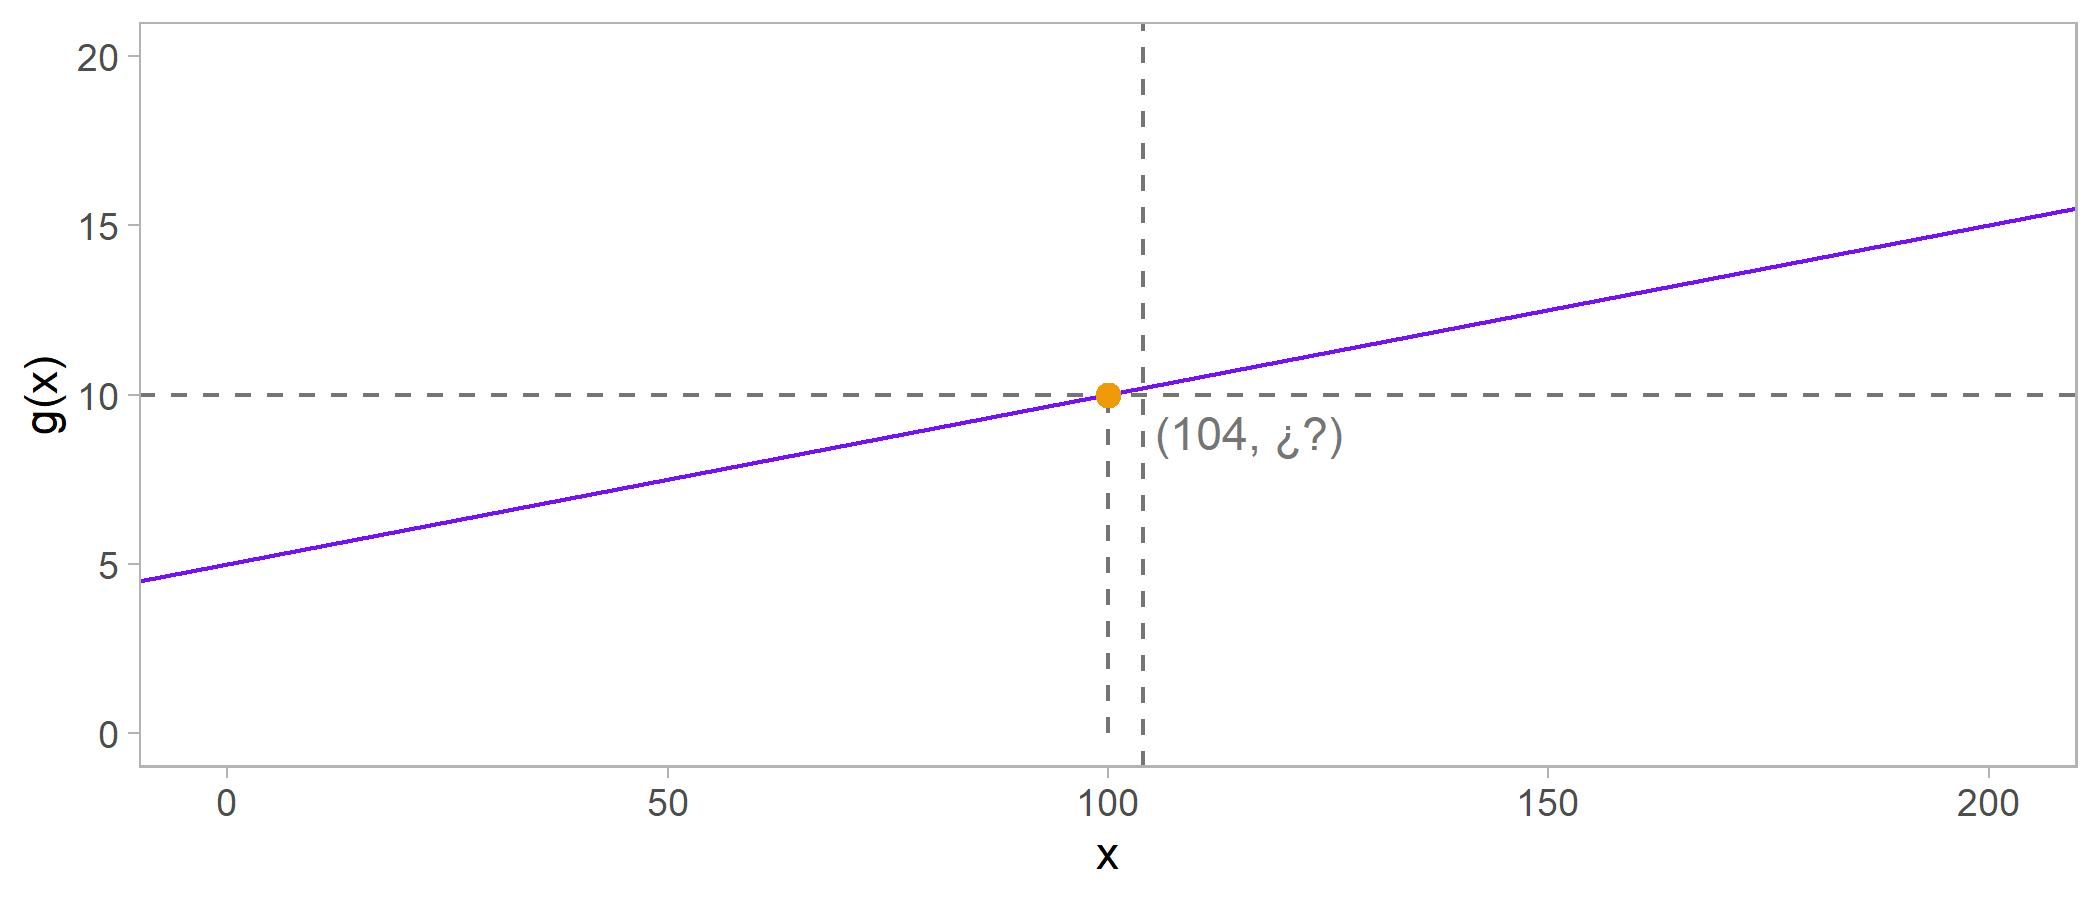
\includegraphics[scale=0.7]{img/approx_lin_sqrt_2.jpg}
\end{figure}

Una estrategia que podemos tomar, es aproximarnos al valor de la $\sqrt{104}$ a través de la línea tangente, tal como lo hicimos antes, lo cual implica que asumiremos que dicha línea es constante.

Entonces, en primer lugar, calculamos la distancia horizontal que hay entre $x = 104$ y $x = 100$, la cual es igual a $4$. Luego, podemos obtener la distancia vertical que hay entre $g(100) = 10$ y $g(104)$, por medio del producto entre la pendiente de la línea tangente ($0.05$) y la distancia horizontal que acabamos de calcular ($4$). Como vemos en la siguiente imagen del mismo gráfico anterior\footnote{Acorté las escalas de ambos ejes, para que pueda ser más visible lo que se explica.}, dicha multiplicación es igual a $0.2$.

\begin{figure}[hbt!]
\centering
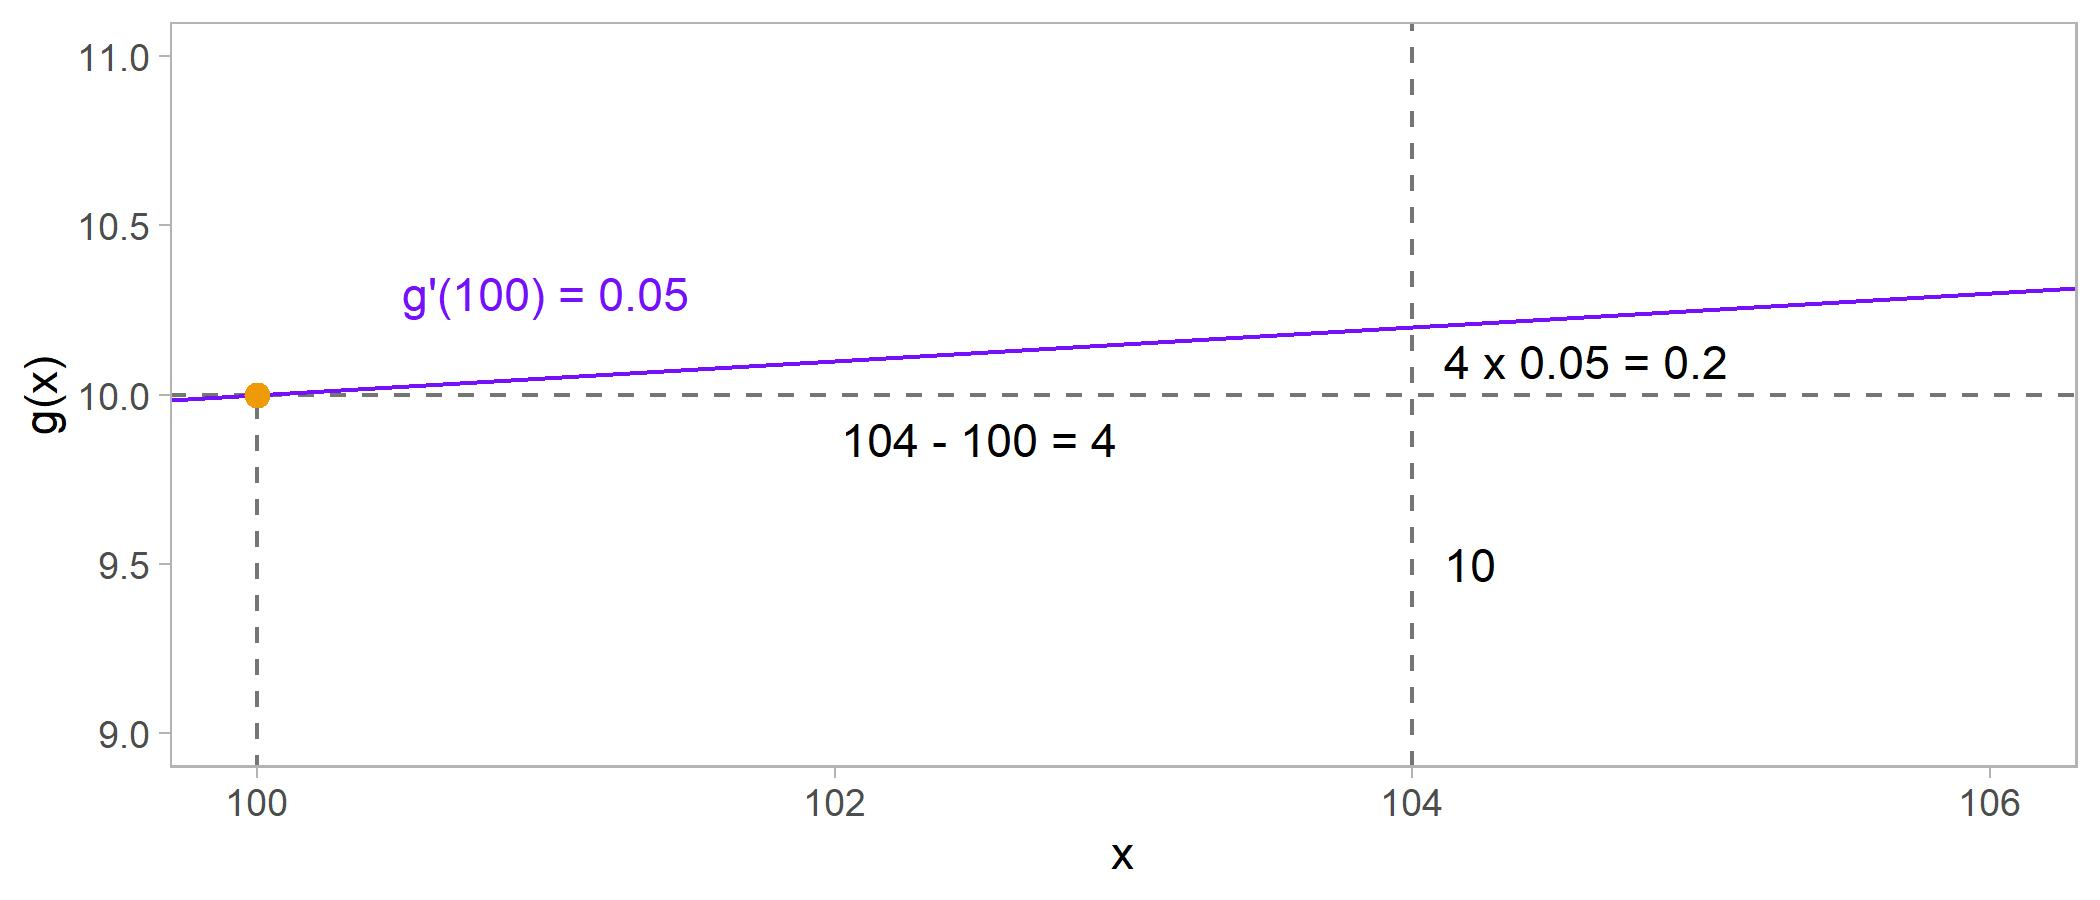
\includegraphics[scale=0.7]{img/approx_lin_sqrt_3.jpg}
\end{figure}

Con todo, lo que nos queda para obtener el valor aproximado de la $\sqrt{104}$ o el \textit{output} de $g(104)$, es simplemente sumar la distancia vertical entre $g(104)$ y $g(100)$ (i.e., $0.2$), más $g(100)$. Es decir:
\[g(104) \approx 10 + 0.2\]
\[g(104) \approx 10.2\]
Por lo tanto, la $\sqrt{104}$ se aproxima a $10.2$. Y si dicho valor lo buscamos en una calculadora, veremos que se acerca bastante al resultado que obtuvimos ($10.198036...$). 

Ahora veamos en términos más generales la definición de la aproximación lineal.

Digamos que queremos estimar una función $g(x)$ en $x$ y el punto en donde comienza es $x_{0}$, lo que significa que la altura de este último valor es $g(x_{0})$. La distancia entre $x$ y $x_{0}$, es $\Delta \, x$ y la pendiente de la línea tangente será $m = g'(x_{0})$.

\begin{figure}[hbt!]
\centering
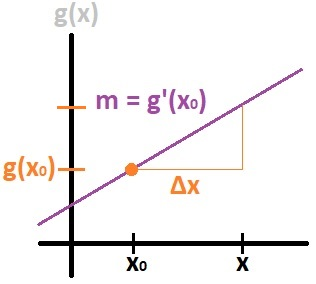
\includegraphics[scale=0.7]{img/approx_lin_gral_expl.jpg}
\end{figure}

Por consiguiente, la distancia vertical entre $g(x_{0})$ y el valor de la función $g(x)$ que buscamos estimar con el valor de $x$ (i.e., $\Delta \, g$) será, aproximadamente, el producto entre la pendiente de la línea tangente ($m$) y la distancia $\Delta \, x$.

\newpage

\begin{figure}[hbt!]
\centering
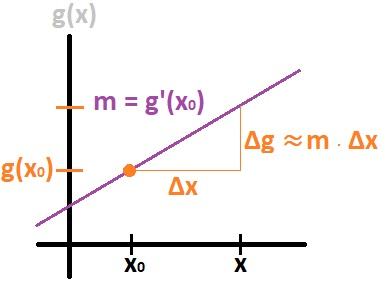
\includegraphics[scale=0.7]{img/approx_lin_gral_expl_2.jpg}
\end{figure}

Juguemos un poco con la expresión $\Delta \, g \approx m \cdot \Delta \, x$.
\[\Delta \, g \approx m \cdot \Delta \, x\]
\[g(x) - g(x_{0}) \approx g'(x_{0}) \cdot (x - x_{0})\]
\[g(x) \approx g'(x_{0}) \cdot (x - x_{0}) + g(x_{0})\]
Acá nos encontramos con dos fórmulas:

\begin{itemize}
\item Lado izquierdo $\rightarrow$ $g(x)$ = Fórmula del gráfico.
\item Lado derecho $\rightarrow$ $g'(x_{0}) \cdot (x - x_{0}) + g(x_{0})$ = Fórmula de la línea tangente.
\end{itemize}

En otras palabras, podemos decir que:

\centerline{Fórmula Gráfico $\approx$ Fórmula Línea Tangente}

Y dicha afirmación es \textbf{verdadera cuando $x$ es cercano a $x_{0}$}.

Todo esto proviene de la \textbf{definición de la derivada}. Sabemos que la pendiente de la línea tangente ($m$) corresponde a:
\[m = \lim_{\Delta \, x \to 0} \frac{\Delta \, g}{\Delta \, x}\]

\newpage

Lo cual también podemos interpretar como:

\centerline{$m \approx \Delta \, g/\Delta \, x$ cuando $\Delta \, x$ es pequeño (i.e., cuando es cercano a cero).}

Por lo tanto, si despejamos $\Delta \, g$ de aquella expresión:
\[m \approx \frac{\Delta \, g}{\Delta \, x}\]
\[m \cdot \Delta \, x \approx \Delta \, g\]
Entonces volvemos a la expresión que vimos en el último gráfico (pág. 10) y que \textbf{corresponde a la aproximación lineal}.

Podemos definir más formalmente la aproximación lineal de una función:

La aproximación lineal para una función $f$ cercana a un punto $x = a$, está dada por las siguientes fórmulas equivalentes:
\[\mathrm{(1)} \, \Delta f \approx \diff*{f(x)}x[x=a] \cdot \Delta \, x; \qquad \mathrm{para} \, \Delta \, x \, \mathrm{cercano} \, \mathrm{a} \, 0\]
\[\mathrm{(2)} \, f(x) \approx f'(a)(x - a) + f(a); \qquad \mathrm{para} \, x \, \mathrm{cercano} \, \mathrm{de} \, ``a''\]

\underline{Veamos otro ejemplo}: Use la aproximación lineal para estimar, \textbf{sin calculadora}, el valor de $3.97^{2.5}$.

A diferencia del ejercicio que realizamos anteriormente (págs 6-9), acá simplemente nos dan la expresión, pero no a partir de una función. No obstante, podemos asumirla como una función más general:
\[f(x) = x ^{2.5}\]
¿Por qué escogimos expresar de esa manera la función? Porque ya sabemos cómo calcular la derivada de una potencia, entonces podemos seguir este camino. Recordemos que, en las fórmulas de la aproximiación lineal, tenemos que calcular la derivada de una función en un punto y, como ya hemos visto, lo mejor es partir calculando la derivada en general.

Dicho eso, calculemos la derivada de $f(x)$.
\[\diff*{f(x)}x = (x^{2.5})'\]
\[\diff*{f(x)}x = 2.5(x^{2.5 - 1})\]
\[\diff*{f(x)}x = 2.5(x^{1.5})\]
\[\diff*{f(x)}x = \frac{5}{2}(x^{3/2})\]
\[\diff*{f(x)}x = \frac{5}{2}(\sqrt{x^{3}})\]
\[\diff*{f(x)}x = \frac{5x \sqrt{x}}{2}\]
Ahora que hemos calculado la derivada de $f(x)$, antes de calcular la aproximación lineal, tenemos que escoger tanto un valor para $x$ como para $a$, en donde $x$ debe ser muy cercano a $a$. El valor $x$ es el que vamos a estimar, que en este caso corresponde a $3.97$; mientras que $a$ debe ser muy cercano a $3.97$. En esta ocasión, diremos que $a = 4$, puesto que es un valor cerrado y muy cercano a $3.97$. En otras palabras:

\begin{itemize}
\item $x = 3.97$
\item $a = 4$
\end{itemize}

Ahora apliquemos esta información a la fórmula de aproximación lineal:
\[f(x) \approx f'(a)(x - a) + f(a)\]
\[f(x) \approx \frac{5a \sqrt{a}}{2} \cdot (x - a) + a^{2.5}\]
\[f(x) \approx \frac{5a \sqrt{a}}{2} \cdot (x - a) + a^{2}\sqrt{a}\]
\[f(3.97) \approx \frac{5 \cdot 4 \sqrt{4}}{2} \cdot (3.97 - 4) + 4^{2}\sqrt{4}\]
\[f(3.97) \approx 20 \cdot (-0.03) + 32\]
\[f(3.97) \approx -0.6 + 32\]
\[f(3.97) \approx 31.4\]
Por consiguiente, podemos decir que $3.97^{2.5}$ se aproxima a $31.4$, lo cual es correcto si ahora calculamos dicho valor en una calculadora.

A lo largo de esta sección hemos establecido que \textbf{realizar una aproximación lineal en una función} significa usar una \textbf{línea tangente} en su gráfico como \textbf{una estimación para un valor de dicha función} (i.e., para un \textit{output} de ella en un punto). Y esto será correcto \textbf{si la gráfica de dicha función corresponde a aquella línea tangente}. En otras palabras, asumiendo que la línea tangente es \textbf{constante}.

Como sabemos, la mayor parte de las veces las gráficas de las funciones no suelen ser líneas rectas (como una línea tangente), más bien por lo general tienen una o más curvas (pronunciadas en mayor o menor medida) y es debido a ésto que hay una pequeña diferencia entre el valor que aproximamos y el valor real de la función en un punto determinado. En otras palabras, nos referimos a la distancia entre la gráfica y la línea tangente en dicho punto.

Ahora bien, ¿cómo podemos manejar si en el punto que estamos estimando, la función es curvada? Lo podemos hacer a partir de la \textbf{segunda derivada}. Recordemos que la segunda derivada es útil para saber la concavidad de una función en un punto determinado (ver semana 2, págs. 47-50):

\begin{itemize}
\item Si $f''(x) < 0$, entonces $f(x)$ es concava hacia abajo.
\item Si $f''(x) > 0$, entonces $f(x)$ es concava hacia arriba.
\end{itemize}

Por ejemplo, volvamos a ver el caso del primer ejemplo (págs. 6-9). Recordemos información que manejamos de ella:

\newpage

\begin{itemize}
\item $g(x) = \sqrt{x}$ y $g(100) = 10$.
\item $g'(x) = \sqrt{x}/2x$ y $g'(100) = 0.05$
\end{itemize}

Graficamos el punto ($100$, $10$) y la línea tangente como sigue:

\begin{figure}[hbt!]
\centering
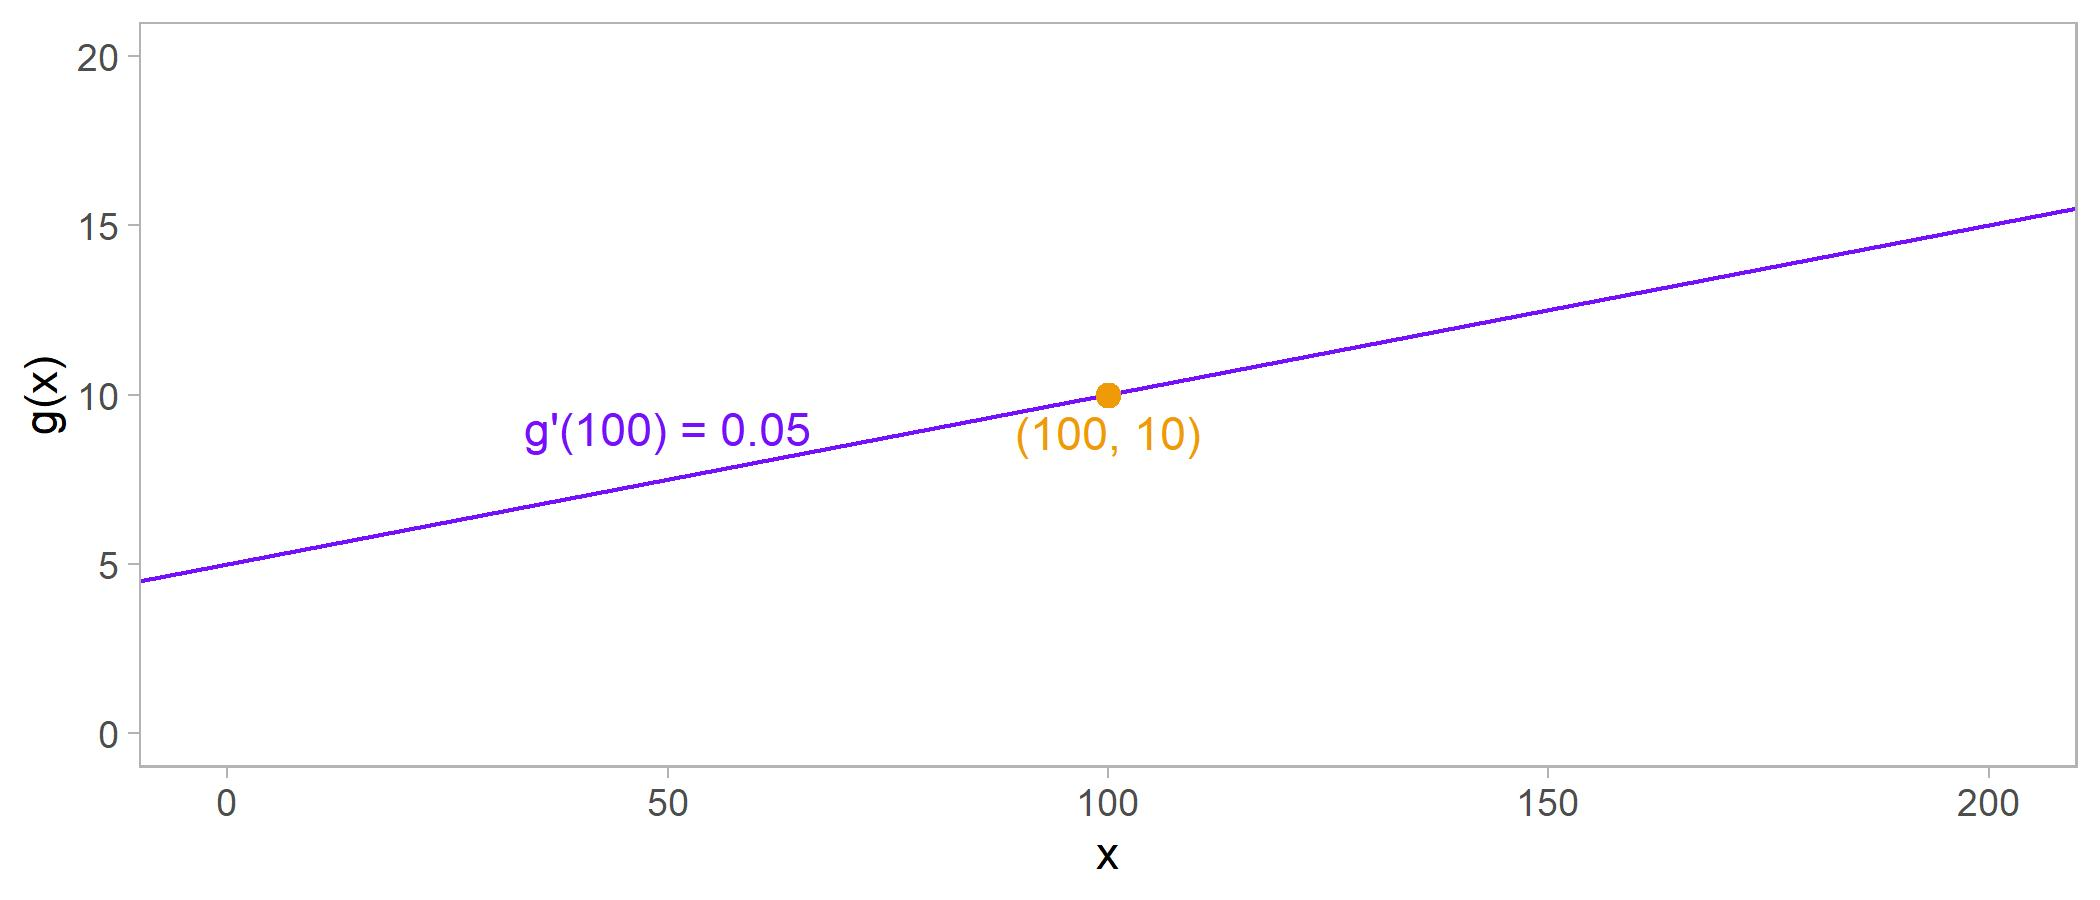
\includegraphics[scale=0.7]{img/approx_lin_sqrt.jpg}
\end{figure}

Y lo que buscábamos era estimar el valor de $\sqrt{104}$ (o $g(104)$), obteniendo que $\sqrt{104} \approx 10.2$.

Ahora calculemos la segunda derivada de $g(x)$ y veamos cuál es su valor en $x = 100$, para ver la concavidad de dicha función en ese punto.
\[\diff*[2]{g(x)}x = \left(\frac{\sqrt{x}}{2x}\right)'\]
Recordemos que $(1/x)' = -1/x^{2}$. Entonces:
\[\diff*[2]{g(x)}x = \frac{-\sqrt{x}}{(2x)^{2}}\]
\[\diff*[2]{g(x)}x = \frac{-\sqrt{x}}{4x^{2}}\]
Calculemos $g''(x)$ en $x = 100$:
\[\diff*[2]{g(x)}x[x = 100] = \frac{-\sqrt{x}}{4x^{2}}\]
\[\diff*[2]{g(x)}x[x = 100] = \frac{-\sqrt{100}}{4 \cdot (100^{2})}\]
\[\diff*[2]{g(x)}x[x = 100] = -0.00025\]
Por lo tanto, podemos decir que en el punto $x = 100$, la gráfica de $g(x)$ es \underline{concava hacia abajo} ($g''(100) < 0$). Esto va a implicar que \textbf{el valor de $g(104)$ va a estar ligeramente abajo del valor que estimamos ($g(104) \approx 10.2$)}. Veámoslo en una calculadora:

\begin{figure}[hbt!]
\centering
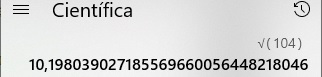
\includegraphics[scale=0.8]{img/approx_lin_sqrt_calc.jpg}
\end{figure}

Como vemos en la imagen de arriba, es un valor muy cercano a $10.2$, nuestra estimación, y está un poco por debajo de este último, tal como lo predecimos a partir del cálculo de la segunda derivada de $g(x)$.

La mayor parte del tiempo cuando le pedimos a un computador que realice este tipo de cálculos, éstas no tienen los valores completos en sus memorias. En efecto, usan técnicas que son similares a la de la aproximación lineal, pero un poco más complejas. No obstante, la aproximación lineal suele ser la base de ellas.

Entonces, hasta el momento hemos estado diciendo que la línea tangente es una buena aproximación de un gráfico, cerca del punto de tangencia, pero ¿a qué nos referimos exactamente con ``cerca''? ¿Qué tan cerca es estar ``cerca''? \textbf{Geométricamente queremos saber qué tan rápido dobla (\textit{blend}), por ejemplo, la gráfica de $g(x)$ de la línea tangente}. Como vemos en la siguiente imagen, ésta puede \underline{doblar lento} (i.e., concavidad es menos pronunciada), lo cual puede implicar que nuestro \textbf{valor estimado no va a estar tan alejado del real}; o puede \underline{doblar rápido} (i.e., concavidad es más pronunciada), que va a significar que nuestro \textbf{valor estimado esté más alejado del valor real}.

\newpage

\begin{figure}[hbt!]
\centering
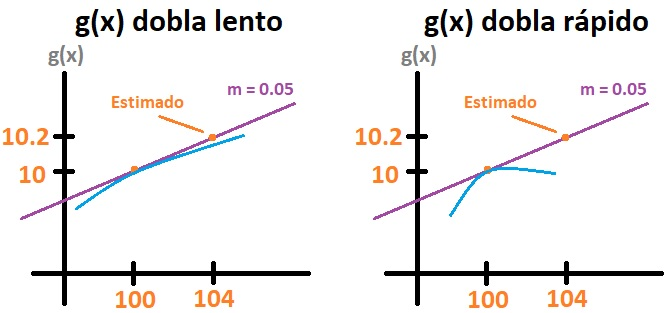
\includegraphics[scale=0.7]{img/approx_lin_blend_lvl.jpg}
\end{figure}

Para saber qué tan rápido o lento dobla la gráfica de una función en un punto determinado, podemos ayudarnos de la \textbf{segunda derivada}. En ese sentido:

\begin{quote}
\centering
Mientras mayor sea el valor de la segunda derivada de una función en un punto determinado, más curvada va a ser su gráfica en dicha posición.
\end{quote}

Volvamos al caso del bote que vimos al inicio (págs. 2-6). En esa ocasión estimamos que su posición $10 \ seg.$ después sería su valor exacto, bajo el supuesto de que la velocidad fuése constante y, por tanto, llegando a ser completamente predecible. Sin embargo, en la realidad el bote no avanzaría de esa manera. Más bien, aceleraría y desaceleraría a medida que va siguiendo su curso y la \textbf{aceleración} corresponde a nuestra \textbf{segunda derivada} en dicho caso.

Basado en el caso del bote que se desplaza en un canal, veamos la siguiente pregunta: ¿Es más fácil de predecir la posición de una canoa o de un barco petrolero (\textit{oil tanker})?

Como recordaremos de nuestras clases de física, en la segunda ley de Newton se señala que, si la masa de un cuerpo es constante, entonces su fuerza resultante es la siguiente:
\[\vec{F} = m \cdot \vec{a} \qquad \mathrm{donde} \ m \ \mathrm{es \ cte}\]
En ese sentido, la \textbf{aceleración ($\vec{a}$)} que adquiere un cuerpo es \textbf{inversamente proporcional a la fuerza ($\vec{F}$)}, en donde la constante de porporcionalidad es la masa ($m$). Por consiguiente, mientras más pesado es el cuerpo, será más difícil que acelere; entonces si es menos pesado, acelerará más fácilmente.

Si comparamos las masas de la canoa como del barco petrolero, la de este último va a ser mayor y, por tanto, acelerará muy poco en comparación a la canoa. Esto implica que \textbf{el gráfico del barco petrolero no será muy curvado} (i.e., su segunda derivada será más chica), por consiguiente, \textbf{su aproximación lineal será más precisa por un periodo más largo de tiempo}, de manera que su posición va a ser más predecible que la de la canoa.




\subsection{Regla del Producto.}

Partamos con las siguientes dos funciones:
\[f(x) = x^{4} \qquad \mathrm{y} \qquad g(x) = sen(x)\]
Como ya sabemos, sus derivadas son:
\[\diff*{f(x)}x = 4x^{3} \qquad \mathrm{y} \qquad \diff*{g(x)}x = cos(x)\]
Estas funciones las podemos sumar
\[f(x) + g(x) = x^{4} + sen(x)\]
Y, también, diferenciar aquella adición, que corresponderá a la suma de ambas derivadas:
\[\diff*{(f(x) + g(x))}x = 4x^{3} + cos(x)\]
Otra operación que podemos realizar entre $f(x)$ y $g(x)$, es \underline{multiplicarlas}.

Digamos que $h(x) = f(x) \cdot g(x)$. Entonces:
\[h(x) = x^{4} \cdot sen(x)\]
Ahora bien, \textbf{¿cómo podemos diferenciar aquel producto?} Podría ser tentador usar el mismo método que usamos en la adición: multiplicar las derivadas de ambas funciones. Sin embargo, \underline{no son iguales}. Es decir:
\[\diff*{h(x)}x \neq \diff*{f(x)}x \cdot \diff*{g(x)}x\]
Veamos el motivo de la afirmación anterior. Digamos que tenemos las siguientes variables:

\begin{itemize}
\item $t$ $\rightarrow$ Tiempo (en $seg$).
\item $f(t)$ y $g(t)$ $\rightarrow$ Distancias (en $m$).
\item $f'(t)$ y $g'(t)$ $\rightarrow$ Velocidades (en $m/s$).
\item $h(t) = f(t) \cdot g(t)$ $\rightarrow$ Área (en $m^{2}$).
\end{itemize}

Visualizaremos lo anterior en un rectángulo, donde el ancho será $f(t)$ y la altura $g(t)$.

\newpage

\begin{figure}[hbt!]
\centering
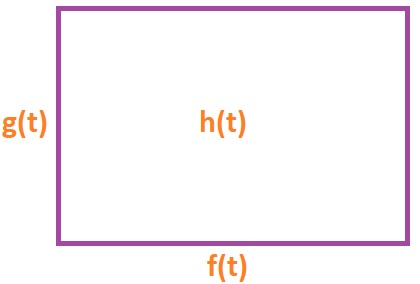
\includegraphics[scale=0.7]{img/deriv_prod_examp.jpg}
\end{figure}

Nuestro propósito es ver qué ocurre con $h'(t)$. La función $h(t)$ es medida en $m^{2}$, mientras que el \textit{input} en $h'(t)$ es medido en $seg$, de manera que \textbf{el \textit{output} de $h'(t)$ deberá ser medido en $m^{2}/s$}.
\[h'(t) = \mathrm{``algo''} \ \frac{m^{2}}{s}\]
Sin embargo, si multiplicamos $f'(t)$ y $g'(t)$, su resultado será medido de la siguiente forma:
\[f'(t) \cdot g'(t) = \mathrm{``algo''} \ \left(\frac{m}{s} \cdot \frac{m}{s}\right)\]
\[f'(t) \cdot g'(t) = \mathrm{``algo''} \ \frac{m^{2}}{s^{2}}\]
En otras palabras, $h'(t)$ y $f'(t) \cdot g'(t)$, no calzan, ya que \textbf{ambas derivadas miden cosas distintas}. Es decir:
\[\diff*{h(x)}x \neq \diff*{f(x)}x \cdot \diff*{g(x)}x\]
Porque:
\[\frac{m^{2}}{s} \neq \frac{m^{2}}{s^{2}}\]
Entonces, esto nos lleva a preguntarnos ¿qué es $h'(t)$? Sabemos que $h(t)$ mide el área, en este caso, del rectángulo. Por consiguiente, $h'(t)$ será \textbf{la tasa de cambio del área}.

Para entender mejor ésto, démosle algunos valores a los datos con los que estamos trabajando:

\begin{itemize}
\item $t = 3 \ seg$.
\item $f(3) = 50 \ m$ y $g(3) = 30 \ m$.
\item $f'(3) = 4 \ m/s$ y $g'(3) = 2 \ m/s$.
\end{itemize}

Integremos estos valores al rectángulo donde estamos visualizando aquello.

\begin{figure}[hbt!]
\centering
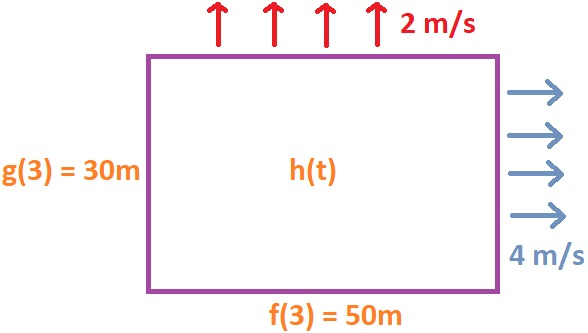
\includegraphics[scale=0.7]{img/deriv_prod_examp_2.jpg}
\end{figure}

Lo que queremos ver \textbf{en $h'(3)$ es la tasa de cambio de dicha área} o, en otras palabras, qué tan rápido cambia el área $h(t)$, en $t = 3 \ seg$. Como podemos observar, en $f'(3)$ estamos ensanchándo hacia la derecha el área a una velocidad de $4 \ m/s$, mientras que en $g'(3)$, el área del rectángulo se está alargando hacia arriba a una tasa de $2 \ m/s$. Esto lo podemos expresar de la siguiente manera:

\begin{itemize}
\item Ensanchamiento hacia la derecha $\rightarrow$ $30 \ m \cdot 4 \ m/s$.
\item Alargamiento hacia arriba $\rightarrow$ $50 \ m \cdot 2 \ m/s$.
\end{itemize}

Si calculamos ambas multiplicaciones, entonces obtendremos respectivamente:

\begin{itemize}
\item Ensanchamiento hacia la derecha $\rightarrow$ $120 \ m^{2}/s$.
\item Alargamiento hacia arriba $\rightarrow$ $100 \ m^{2}/s$.
\end{itemize}

Entonces, para obtener $h'(3)$ o la tasa de cambio del área en $t = 3s$, simplemente debemos sumar los dos productos que acabamos de obtener.
\[h'(3) = 120 \ \frac{m^{2}}{s} + 100 \ \frac{m^{2}}{s}\]
\[h'(3) = 220 \ \frac{m^{2}}{s}\]
Por consiguiente, la tasa de cambio del área del rectángulo en $t = 3 \ s$, fue de $220 \ m^{2}/s$.

Ahora, generalicemos el cálculo que acabamos de realizar. Recordemos los datos con los que trabajamos:

\begin{itemize}
\item $f(3) = 50 \ m$.
\item $f'(3) = 4 \ m/s$.
\item $g(3) = 30 \ m$.
\item $g'(3) = 2 \ m/s$.
\end{itemize}

Por lo tanto, hicimos el siguiente cálculo para encontrar $h'(3)$:
\[h'(3) = f(3) \cdot g'(3) + g(3) \cdot f'(3)\]
Y, justamente como lo necesitábamos, el resultado fue medido en $m^{2}/s$.

Entonces, en términos generales podemos decir que si:
\[h(x) = f(x) \cdot g(x)\]
Por consiguiente, \textbf{la derivada de $h(x)$}, será:
\[h'(x) = f'(x) \cdot g'(x) + g(x) \cdot f'(x)\]
Y esto es verdadero en todos los puntos en donde las derivadas de $f(x)$ y $g(x)$, existen. A esto se le denomina como la \textbf{\underline{regla del producto}}.

Apliquemos esta regla a las funciones que vimos al inicio de esta sección.
\[f(x) = x^{4} \qquad y \qquad g(x) = sen(x)\]
Sea $h(x) = f(x) \cdot g(x)$, calculemos $h'(x)$.
\[h'(x) = f(x) \cdot g'(x) + g(x) \cdot f'(x)\]
\[h'(x) = x^{4} \cdot cos(x) + sen(x) \cdot 4x^{3}\]

Ahora veamos \textbf{más formalmente la regla del producto}, a partir de la notación \textit{delta} (i.e, $\Delta$). Como vimos, $h(t)$ corresponde al siguiente producto entre funciones:
\[h(t) = f(t) \cdot g(t)\]
Haciendo uso de la notación \textit{delta}, la derivada de $h(t)$ la podemos expresar de la siguiente manera:
\[h'(t) \approx \frac{\Delta h}{\Delta t}\]
Y, para obtener el resultado exacto de $h'(t)$, vamos a tomar su límite a medida que $\Delta t \to 0$.

Concentrémonos en el \underline{numerador de $h'(t)$: $\Delta h$}. Éste valor corresponde al cambio en $h$. Es decir, a la diferencia entre el valor nuevo de $h$ (el que cambió) y su valor anterior.
\[\Delta h = \mathrm{nuevo} \ h - \mathrm{viejo} \ h\]
Sabemos que $h$ cambia cuando $f$ y $g$ cambian. Como $h$ siempre es igual al producto entre $f$ y $g$, entonces el \textbf{valor nuevo de $h$} será $(f + \Delta f)(g + \Delta g)$. Mientras que el \textbf{viejo valor de $h$} va a corresponder a su valor original, que corresponde a $f \cdot g$. En otras palabras, $\Delta h$ corresponde a la siguiente expresión:
\[\Delta h = (f + \Delta f)(g + \Delta g) - f \cdot g\]
Esto también lo podemos visualizar en un rectángulo.

\begin{figure}[hbt!]
\centering
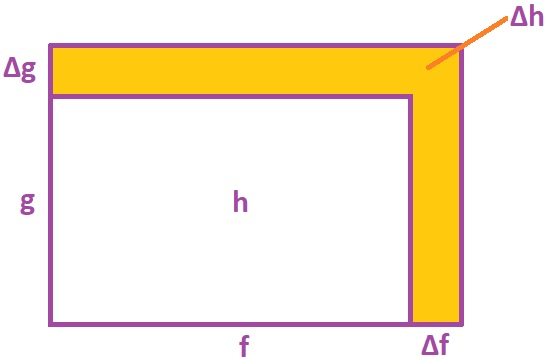
\includegraphics[scale=0.6]{img/formal_prod_rule.jpg}
\end{figure}

Como vemos, toda el área naranja que se genera a partir del alargamiento de $g$, que es igual a ($g + \Delta g$); y de $f$, cuyo valor es ($f + \Delta h$), corresponde al cambio en $h$ o, en otras palabras, a $\Delta h$, luego de haber restado dichos alargamientos al área original de $h$, es decir, a $g \cdot f$.

Ahora bien, en la última imagen de arriba estamos asumiendo que $g$, $\Delta g$, $f$ y $\Delta f$, son cantidades positivas. Sin embargo, en álgebra no existe tal supuesto; en efecto, es mucho más general y formal. En ese sentido, la imagen solo nos sirve para tener una idea intuitiva de los términos que se están tratando.

Volvamos al álgebra en la expresión de $\Delta h$:
\[\Delta h = (f + \Delta f)(g + \Delta g) - f \cdot g\]
\[\Delta h = f \cdot g + f \cdot \Delta g + \Delta f \cdot g + \Delta f \cdot \Delta g - f \cdot g\]
\[\Delta h = f \cdot \Delta g + \Delta f \cdot g + \Delta f \cdot \Delta g\]
Las expresiones que vemos en el cálculo de $\Delta h$, los podemos encontrar en la imagen del rectángulo de arriba:

\newpage

\begin{figure}[hbt!]
\centering
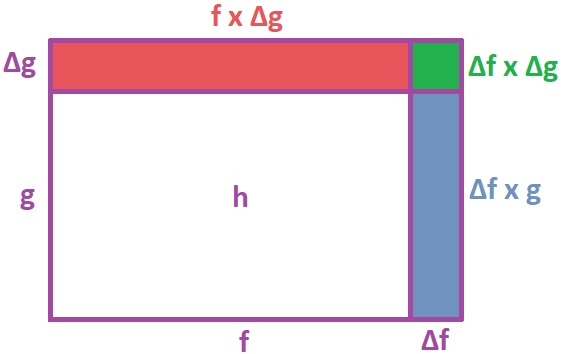
\includegraphics[scale=0.6]{img/formal_prod_rule_2.jpg}
\end{figure}

Volvamos a la expresión $\Delta h / \Delta t$. Ya conocemos la expresión de $\Delta h$, así que agreguémosla a la ecuación:
\[h'(t) \approx \frac{\Delta h}{\Delta t}\]
\[h'(t) \approx \frac{f \cdot \Delta g + \Delta f \cdot g + \Delta f \cdot \Delta g}{\Delta t}\]
Esto es lo mismo que:
\[h'(t) \approx \left(f \cdot \frac{\Delta g}{\Delta t}\right) + \left(\frac{\Delta f}{\Delta t} \cdot g\right) + \left(\frac{\Delta f}{\Delta t} \cdot \frac{\Delta g}{\Delta t} \cdot \Delta t\right)\]
Recordemos que de esta expresión vamos a calcular el límite a medida que $\Delta t \to 0$:
\[h'(t) = \lim_{\Delta t \to 0} \frac{\Delta h}{\Delta t}\]
Que será lo mismo a:
\[h'(t) = \lim_{\Delta t \to 0} \left[\left(f \cdot \frac{\Delta g}{\Delta t}\right) + \left(\frac{\Delta f}{\Delta t} \cdot g\right) + \left(\frac{\Delta f}{\Delta t} \cdot \frac{\Delta g}{\Delta t} \cdot \Delta t\right)\right]\]
\[h'(t) = \left(\lim_{\Delta t \to 0} f \cdot \frac{\Delta g}{\Delta t}\right) + \left(\lim_{\Delta t \to 0} \frac{\Delta f}{\Delta t} \cdot g\right) + \left(\lim_{\Delta t \to 0} \frac{\Delta f}{\Delta t} \cdot \frac{\Delta g}{\Delta t} \cdot \Delta t\right)\]
\[h'(t) = f \cdot \left(\lim_{\Delta t \to 0} \frac{\Delta g}{\Delta t}\right) + g \cdot \left(\lim_{\Delta t \to 0} \frac{\Delta f}{\Delta t}\right) + \left(\lim_{\Delta t \to 0} \frac{\Delta f}{\Delta t} \cdot \frac{\Delta g}{\Delta t} \cdot 0\right)\]
\[h'(t) = f \cdot \left(\lim_{\Delta t \to 0} \frac{\Delta g}{\Delta t}\right) + g \cdot \left(\lim_{\Delta t \to 0} \frac{\Delta f}{\Delta t}\right) + \left(\lim_{\Delta t \to 0} 0\right)\]
\[h'(t) = f \cdot g' + g \cdot f'\]

De esta manera, entonces obtenemos la \underline{regla del producto}.




\subsection{Regla del Cuociente.}

En esta ocasión digamos que tenemos la siguiente función:
\[h(t) = \frac{f(t)}{g(t)}\]
y queremos buscar su derivada o $h'(t)$.

Del mismo modo a cómo lo vimos al inicio de la sección anterior, el valor de $h'(t)$ no puede ser el cálculo del siguiente valor:
\[h'(t) \neq \frac{f'(t)}{g'(t)}\]
Esto se debe a que las unidades de $h'(t)$ y de la división entre $f'(t)$ y $g'(t)$, no son iguales.

Entonces, para buscar cuál es, realmente, la derivada de la función $h(t)$, lo haremos del mismo modo en que lo hicimos en la regla del producto. Es decir, tomaremos el enfoque de la \underline{aproximación lineal}, por lo que diremos que:
\[h'(t) \approx \frac{\Delta h}{\Delta t} \ \mathrm{cuando} \ \Delta t \ \mathrm{es \ chico}\]
Por otra parte, también buscaremos el valor de $\Delta t$ en términos de $f$, $\Delta f$, $g$ y $\Delta g$; y, finalmente, tomaremos el límite de toda la expresión. Es decir:
\[h'(t) = \lim_{\Delta t \to 0} \frac{\Delta h}{\Delta t}\]
con lo que obtendremos la fórmula de la \textbf{regla del cuociente}.

Partamos con $\Delta h$. Al igual que como lo vimos cuando buscábamos la fórmula de la regla del producto, dijimos que el valor del denominador era igual a la diferencia entre el valor nuevo de $h$ y el viejo $h$.
\[h'(t) = \lim_{\Delta t \to 0} \frac{\Delta h}{\Delta t}\]
\[h'(t) = \lim_{\Delta t \to 0} \frac{\mathrm{nuevo} \ h - \mathrm{viejo} \ h}{\Delta t}\]
Entonces, como:
\[h = \frac{f}{g}\]
La expresión de $\Delta h$ será:
\[h'(t) = \lim_{\Delta t \to 0} \frac{\frac{f + \Delta f}{g + \Delta g} - \frac{f}{g}}{\Delta t}\]
Para hacer más visible el cálculo de $\Delta h$, realicémoslo de forma separada:
\[\Delta h = \frac{f + \Delta f}{g + \Delta g} - \frac{f}{g}\]
\[\Delta h = \frac{g(f + \Delta f) - f(g + \Delta g)}{g(g + \Delta g)}\]
\[\Delta h = \frac{g \cdot f  + g \cdot \Delta f - f \cdot g - f \cdot \Delta g}{g^{2} + g \cdot \Delta g}\]
Los valores $g \cdot f$ y $- f \cdot g$, se cancelan, por lo que:
\[\Delta h = \frac{g \cdot \Delta f - f \cdot \Delta g}{g^{2} + g \cdot \Delta g}\]
Entonces, de momento $h'(t)$ nos está quedando así:
\[h'(t) = \lim_{\Delta t \to 0} \frac{\frac{g \cdot \Delta f - f \cdot \Delta g}{g^{2} + g \cdot \Delta g}}{\Delta t}\]
Lo cual es lo mismo que:
\[h'(t) = \lim_{\Delta t \to 0} \left(\frac{g \cdot \Delta f - f \cdot \Delta g}{g^{2} + g \cdot \Delta g} \cdot \frac{1}{\Delta t}\right)\]
\[h'(t) = \lim_{\Delta t \to 0} \left(\frac{g \cdot \Delta f - f \cdot \Delta g}{\Delta t} \cdot \frac{1}{g^{2} + g \cdot \Delta g}\right)\]
Como sabemos, el límite de una multiplicación entre dos valores es igual al producto al límite de un valor y el límite del otro, en donde ambos tienden a un mismo valor. Es decir:
\[h'(t) = \left(\lim_{\Delta t \to 0} \frac{g \cdot \Delta f - f \cdot \Delta g}{\Delta t}\right) \cdot \left(\lim_{\Delta t \to 0} \frac{1}{g^{2} + g \cdot \Delta g}\right)\]
Calculemos los límites de ambas expresiones:
\[h'(t) = \left[\left(\lim_{\Delta t \to 0} g \cdot \frac{\Delta f}{\Delta t}\right) - \left(\lim_{\Delta t \to 0} f \cdot \frac{\Delta g}{\Delta t}\right)\right] \cdot \left[\lim_{\Delta t \to 0} \frac{1}{g^{2} + g \cdot \Delta g}\right]\]
\[h'(t) = \left[g \cdot \left(\lim_{\Delta t \to 0} \frac{\Delta f}{\Delta t}\right) - f \cdot \left(\lim_{\Delta t \to 0} \frac{\Delta g}{\Delta t}\right)\right] \cdot \left[\lim_{\Delta t \to 0} \frac{1}{g^{2} + g \cdot \Delta g}\right]\]
\[h'(t) = [g \cdot f' - f \cdot g'] \cdot \left[\lim_{\Delta t \to 0} \frac{1}{g^{2} + g \cdot \Delta g}\right]\]
\[h'(t) = \frac{g \cdot f' - f \cdot g'}{\lim_{\Delta t \to 0} (g^{2} + g \cdot \Delta g)}\]
El límite de $\Delta g$ a medida que $\Delta t \to 0$, es igual a cero, lo que implica que $g \cdot \Delta g$ también será igual a cero.
\[h'(t) = \frac{g \cdot f' - f \cdot g'}{g^{2} + 0}\]
Por lo tanto, la \textbf{regla del cuociente} se define como sigue:
\[h'(t) = \left(\frac{f}{g}\right)' = \frac{g \cdot f' - f \cdot g'}{g^{2}}\]
Y el valor de la $h'(t)$ será verdadero cuando:

\begin{enumerate}
\item Las derivadas de $f(t)$ y $g(t)$, o $f'(t)$ y $g'(t)$, existan.
\item $(g(t))^{2} \neq 0$
\end{enumerate}

Veamos ahora el siguiente ejemplo: Calculemos la derivada de la $tan(x)$.

Como sabemos, la $tan(x)$ se define como:
\[tan(x) = \frac{sen(x)}{cos(x)}\]
Entonces, si aplicamos la regla del cuociente:
\[\diff*{tan(x)}x = \frac{cos(x) \cdot (sen(x))' - sen(x) \cdot (cos(x))'}{cos^{2}(x)}\]
\[\diff*{tan(x)}x = \frac{cos(x) \cdot cos(x) - sen(x) \cdot (-sen(x))}{cos^{2}(x)}\]
\[\diff*{tan(x)}x = \frac{cos(x) \cdot cos(x) + sen(x) \cdot sen(x)}{cos^{2}(x)}\]
\[\diff*{tan(x)}x = \frac{cos^{2}(x) + sen^{2}(x)}{cos^{2}(x)}\]
Como podemos apreciar, en el numerador nos encontramos con la identidad pitagórica:
\[sen^{2}(x) + cos^{2}(x) = 1\]
Entonces:
\[\diff*{tan(x)}x = \frac{1}{cos^{2}(x)}\]
Si recordamos las identidades trigonométricas, la correspondiente a la $sec(x)$ era la inversa del $cos(x)$:
\[sec(x) = \frac{1}{cos(x)}\]
Por lo tanto, podemos decir que la derivada de la $tan(x)$ será:
\[\diff*{tan(x)}x = \left(\frac{1}{cos(x)}\right)^{2}\]
\[\diff*{tan(x)}x = sec^{2}(x)\]

Ya hemos sabemos cuál es la derivada del $sen(x)$ como del $cos(x)$. Ahora acabamos de calcular la derivada de la $tan(x)$ usando la regla del cuociente. Usando esta misma regla, podemos encontrar las derivadas de las restantes funciones trigonométricas, las cuales resumimos a continuación:
\[\diff*{sen(x)}x = cos(x)\]
\[\diff*{cos(x)}x = -sen(x)\]
\[\diff*{tan(x)}x = \frac{1}{cos^{2}(x)} = sec^{2}(x)\]
\[\diff*{cot(x)}x = \frac{1}{sen^{2}(x)} = csc^{2}(x)\]
\[\diff*{sec}x = \frac{sen(x)}{cos^{2}(x)} = sec(x) \cdot tan(x)\]
\[\diff*{csc}x = - \frac{cos(x)}{sen^{2}(x)} = -csc(x) \cdot cot(x)\]




\subsection{Regla de la Cadena.}

Comencemos con el siguiente ejemplo.

Supongamos que la variable $x$ mide en metros la posición de una bicicleta a lo largo de un camino. También, la cantidad de tiempo recorrido desde el comienzo del viaje se mide a partir de la variable $t$ en segundos, y con la variable $u$ se mide lo mismo, pero en minutos.

En primer lugar, ¿cuál es la relación que hay entre $u$ y $t$?

Como se señaló, tanto $u$ como $t$ miden el tiempo recorrido desde el inicio del viaje, pero uno en minutos y el otro en segundos, respectivamente. Sabemos que $1 \ \mathrm{min} = 60 \ \mathrm{seg}$, entonces podemos decir que:
\[u = 60t\]
Podemos también calcular la derivada de $u$, puesto que está en función de $t$. En otras palabras, estará medida en $seg/min$:
\[\diff*{u}t = (60t)'\]
\[\diff*{u}t = 60 \ s/min\]
El valor de $u'$ corresponde al \textbf{factor de conversión}. En este caso, de segundos a minutos. Profundizaremos en esto más adelante.

En segundo lugar, la posición $x$ está en función del tiempo. Para este caso, ésto quiere decir que $x$ puede estar en función de $u$ o de $t$. Entonces, para distinguirlas, digamos que:

\begin{itemize}
\item $x = f(u)$
\item $x = g(t)$
\end{itemize}

Por lo tanto, sea la función $f(u) = 2u + 100$, ¿cuál es el valor de $\frac{dx}{du}$?

Como vemos, nos están pidiendo la derivada de $x$ en función de $u$. En otras palabras, $f'(u)$:
\[\diff*{x}u = \diff*{f(u)}u = (2u + 100)'\]
\[\diff*{f(u)}u = (2u)' + (100)'\]
\[\diff*{f(u)}u = 2(u)' + 0\]
\[\diff*{f(u)}u = 2\]
Como estamos midiendo el cambio instantáneo de $f(u)$ y $u$ es medido en $seg$, entonces $\frac{d}{du}f(u)$ es medido en $m/seg$. Es decir:
\[\diff*{f(u)}u = 2 \ m/s\]
Ahora, en tercer lugar, dado que ya conocemos la fórmula de $x$ en términos de $u$ (i.e., $f(u) = 2u + 100$), entonces ¿cuál es la fórmula de $x$ en términos de $t$?

En esta ocasión, nos piden la fórmula de $g(t)$. Como sabemos, la relación entre $u$ y $t$ es $u = 60t$. Como ambas son $inputs$ de la medida de la misma distancia $x$, pero medida en unidades de tiempo diferentes, entonces podemos decir que:
\[g(t) = f(60t)\]
\[g(t) = 2 \cdot (60t) + 100\]
\[g(t) = 120t + 100\]
Finalmente, ¿cuál es la $\frac{dx}{dt}$?

Al igual como lo hicimos con $f(u)$, ahora calculamos la derivada de $g(t)$:
\[\diff*{x}t = \diff*{g(t)}t = (120t + 100)'\]
\[\diff*{g(t)}t = (120t)' + (100)'\]
\[\diff*{g(t)}t = 120\]
Recordemos que $t$ es medido en minutos. Por lo tanto:
\[\diff*{g(t)}t = 120 \ m/min\]
A lo largo de este ejemplo hemos dicho que la posición de la bicicleta $x$ (en $m$) que viaja en un camino, está en función del tiempo. Dicho tiempo lo medimos tanto en minutos, a partir de la variable $t$, como en segundos, por medio de la variable $u$. Para distinguir la medición de ambas distancias, dijimos que para el caso en donde el tiempo se mide en minutos, esta correspondería a $f(u)$, mientras que el tiempo en segundos, la posición se medía a partir de $g(t)$. Por lo tanto, podemos afirmar que:
\[x = g(t) = f(u)\]
Podemos señalar lo expresado arriba, ya que las tres distancias (o posiciones de la bicicleta), se miden en metros. No obstante, cuando medimos \textbf{cuánto cambia la posición por cada unidad de tiempo}, no podemos decir que $f(u)$ y $g(t)$, son iguales. Es decir:
\[\diff*{d(t)}t \neq \diff*{f(u)}u\]
Esto es lo mismo que decir:
\[\diff{x}t \neq \diff{x}u\]
Como vemos, ambas derivadas están en función de dos medidas distintas de tiempo: $t$ y $u$. Entonces, para que sean iguales, tendremos que ajustarlas y es ahí donde es de ayuda el \textbf{factor de conversión} (pág. 30), el cual nos sirve para que la unidad de tiempo de $u$ ($min$) sea igual a la de $t$ ($seg$). Es decir:
\[\diff{x}t = \diff{x}u \cdot \diff{u}t\]
Comprobemos ésto reemplazando las variables de la ecuación de arriba con los valores que hemos obtenido.
\[120 \ \frac{m}{min} = 2 \ \frac{m}{s} \cdot 60 \ \frac{s}{min}\]
\[120 \ \frac{m}{min} = 2 \cdot 60 \ \left(\frac{s}{min} \cdot \frac{m}{s}\right)\]
\[120 \ \frac{m}{min} = 120 \ \frac{m}{min}\]

Ahora veamos ésto usando como enfoque la aproximación lineal a partir del siguiente caso. 

Digamos que tenemos una función $h(x)$ que es una composición de otras dos funciones: $f(x)$ y $g(x)$. Es decir:
\[h(x) = (f \circ g)(x) = f(g(x))\]
Y lo que queremos saber es el valor de $h'(2)$, al menos aproximado.

Supongamos que manejamos los siguientes valores para las 3 funciones:

\begin{itemize}
\item $g(2) = 9$
\item $f(9) = 5$
\item $h(2) = 5$
\end{itemize}

En donde:

\begin{itemize}
\item $2$ se mide en \underline{segundos} ($seg$).
\item $9$ se mide en \underline{metros} ($m$).
\item $5$ se mide en \underline{kilogramos} ($kg$).
\end{itemize}

Para entenderlo mejor, esquematizaremos toda esta información de la siguiente manera:

\begin{figure}[hbt!]
\centering
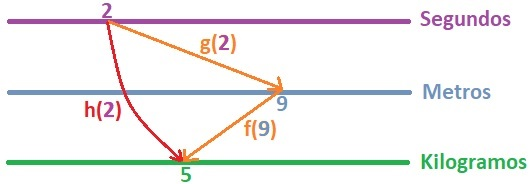
\includegraphics[scale=0.7]{img/intro-chain-rule.jpg}
\end{figure}

Ahora veremos algunas derivadas para $f(x)$ y $g(x)$, y las usaremos para observar cómo se comportan estas funciones cuando sus \textit{inputs} cambian.

Digamos que $g'(2) = 3 \ m/seg$, ¿cuál es nuestra mejor estimación para $g(2.01)$?

Podemos usar la fórmula de \underline{aproximación lineal} (pág. 11) para ver a qué valor se acerca el \textit{output} de $g(2.01)$. Al realizar este cálculo, no olvidemos las unidades de medidas que dimos arriba.
\[g(2.01) \approx g'(2) \cdot (2.01 \ seg - 2 \ seg) + g(2)\]
\[g(2.01) \approx 3 \ \frac{m}{seg} \cdot 0.01 \ seg + 9 \ m\]
\[g(2.01) \approx 0.03 \ m + 9 \ m\]
\[g(2.01) \approx 9.03 \ m\]

Supongamos ahora que $f'(9) = 4 \ kg/m$, ¿cuál es nuestra mejor estimación para $f(g(2.01))$?

Como ya conocemos el valor de $g(2.01)$, entonces podemos decir que $f(g(2.01))$ es lo mismo que $f(9.03)$ y es el \textit{output} de esta última función la que queremos estimar. Entonces, como nos dicen el valor de $f'(9)$ y también manejamos el de $f(9)$, podemos aplicar fácilmente la fórmula de aproximación lineal.
\[f(9.03) \approx f'(9) \cdot (9.03 \ m - 9 \ m) + f(9)\]
\[f(9.03) \approx 4 \ \frac{kg}{m} \cdot 0.03 \ m + 5 \ kg\]
\[f(9.03) \approx 0.12 \ kg + 5 \ kg\]
\[f(9.03) \approx 5.12 \ kg\]
Si observamos bien, acabamos de estimar $f(g(2.01))$, que también es lo mismo que $h(2.01)$. Ya sabemos que $h(2) = 5$, por lo que cuando $h(2)$ se mueve a $h(2.01)$, el \textit{output} se ha movido en $5.12-5 = 0.12 \ kg$. A partir de lo anterior, ¿cuál creemos que debe ser, aproximadamente, el valor de $h'(2)$?

Como sabemos el tanto el valor de $h(2)$ y el aproximado de $h(2.01)$, podemos aprovechar la fórmula de la aproximación lineal para despejar $h'(2)$ y encontrar su valor aproximado.
\[h(2.01) \approx h'(2) \cdot (2.01 \ seg - 2 \ seg) + h(2)\]
\[5.12 \ kg \approx h'(2) \cdot 0.01 \ seg + 5 \ kg\]
\[0.12 \ kg \approx h'(2) \cdot 0.01 \ seg\]
\[\frac{0.12 \ kg}{0.01 \ seg} \approx h'(2)\]
\[12 \ \frac{kg}{seg} \approx h'(2)\]
Entonces, lo que hicimos en este segundo caso fue, para buscar el valor de $h'(2)$, ver qué ocurre con $f(x)$ y $g(x)$ cuando nos movimos de $x = 2 \ seg$ a $x = 2.01 \ seg$, es decir, $\Delta x = 0.01$, y es en este tipo de asuntos en donde las derivadas entran en juego.

En la fórmula de la aproximación lineal (ver pág. 11) nos encontramos con la siguiente expresión:
\[f'(a) \cdot (x - a)\]
Si lo aplicamos a $g(x)$, con $a = 2$ y $x = 2.01$, entonces:
\[g'(2) \cdot (2.01 \ seg - 2 \ seg)\]
Y vimos que ($2.01 \ seg - 2 \ seg$) es $\Delta x$, por lo que:
\[g'(2) \cdot \Delta x\]
Esta expresión corresponde al cambio en la aproximación lineal que ocurre en $g(x)$, es decir, a $\Delta g$. Por lo tanto:
\[\Delta g \approx g'(2) \cdot \Delta x\]
Si reemplazamos con los valores que manejamos:
\[\Delta g \approx 3 \ \frac{m}{seg} \cdot 0.01 \ seg\]
\[\Delta g \approx 0.03 \ m\]
Podemos decir, entonces, que cuando $x$ cambia de $2$ a $2.01$, $g(x)$ cambia en $0.03 \ m$.

Y como estamos en una composición de funciones, donde $h(x) = f(g(x))$, el cambio en $g(x)$ afecta en el cambio en $f(x)$, de manera que:
\[\Delta f \approx f'(9) \cdot \Delta g\]
\[\Delta f \approx 4 \ \frac{kg}{m} \cdot 0.03 \ m\]
\[\Delta f \approx 0.12 \ kg\]
Entonces, cuando $x$ cambia de $2$ a $2.01$, $f(x)$ cambia en $0.12 \ kg$, lo cual implica que dicho cambio también será igual para $h(x)$. Es decir:
\[\Delta h \approx 0.12 \ kg\]
Veamos toda esta nueva información en la siguiente gráfica.

\begin{figure}[hbt!]
\centering
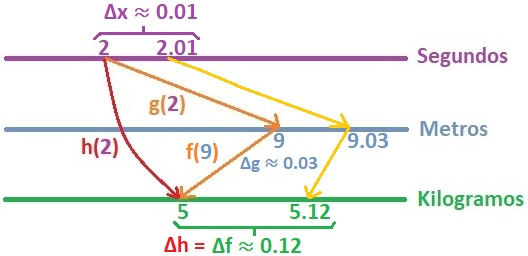
\includegraphics[scale=0.7]{img/intro-chain-rule-2.jpg}
\end{figure}

Ahora tenemos un $\Delta x$ y un $\Delta h$, por consiguiente, podemos calcular la derivada $h'(2)$ a partir de su definición como aproximación a la línea tangente. En otras palabras:
\[h'(2) \approx \frac{\Delta h}{\Delta x}\]
Reemplazando los valores de $\Delta x$ y $\Delta h$:
\[h'(2) \approx \frac{0.12 \ kg}{0.01 \ seg}\]
\[h'(2) \approx 12 \ \frac{kg}{seg}\]
Y, si observamos bien, el resultado de $h'(2)$ es el mismo que el producto entre $f'(9)$ y $g'(2)$. 
\[h'(2) = f'(9) \cdot g'(2)\]
\[h'(2) = 4 \ \frac{kg}{m} \cdot 3 \ \frac{m}{seg}\]
\[h'(2) = 12 \ \frac{kg}{seg}\]
En otras palabras, \textbf{la derivada de una composición de funciones, es igual a la multiplicación entre las derivadas de las funciones que la constituyen}.

Ahora bien, ¿por qué en el cálculo de $h'(2)$ usamos $f'(9)$ y no $f'(2)$? Esto se debe a que $f'(9)$ proviene de $g'(2)$. Lo vimos en el cálculo de $f(9.03)$, el cual se ``alimenta'' de $g(2.01)$ (i.e., $f(g(2.01))$).

El caso que hemos tratado acá, se le denomina como la \underline{\textbf{regla de la cadena}} y se debe a que la aplicamos cuando una función, como $h(x)$, se constituye de dos o más funciones distintas, como $f(x)$ y $g(x)$), las cuales podemos entenderlas como las uniones de $h(x)$.

Lo que descubrimos acá es que, para buscar $h'(x)$, debemos multiplicar las derivadas que componen dicha función. Es decir, obtener el producto entre $f'(x)$ y $g'(x)$, que corresponde a la derivada de la composición total.

Veamos ésto de manera más formal.

Dijimos, entonces, que $h(x)$ es una composición de funciones, las cuales corresponden a $f(x)$ y $g(x)$:
\[h(x) = (f \circ g)(x) = f(g(x))\]
En otras palabras, cuando definimos el \textit{input} $x = a$, entonces obtendremos un \textit{output} $g(a)$ que, a la vez, será el \textit{input} de $f(x)$, cuyo \textit{output} será $f(g(a))$ y que, por consiguiente, será el \textit{output} de $h(x)$. Dicho de otro modo, $f(g(a))$ es el \textit{output} de $h(a)$.

Entonces, para obtener $h(x)$ tenemos una \textbf{variable intermedia} entre el \textit{input} de $x = a$ y $f(x)$, que es $g(x)$. Asignémosles nombres a $g(x)$ y $f(x)$.

\newpage

\begin{itemize}
\item $f(x) = y$
\item $g(x) = u$
\end{itemize}

Podemos decir, a partir de esta notación, que $f(g(x)) = f(u)$ y, por otra parte, como $f(x) = y$, entonces $h(x) = y$.

Pongámoslas en un esquema similar al que hemos usado en esta sección.

\begin{figure}[hbt!]
\centering
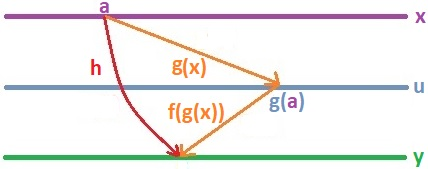
\includegraphics[scale=0.7]{img/intro-chain-rule-3.jpg}
\end{figure}

Nuestro objetivo acá es obtener la derivada de $h(x)$, es decir, cuál es la tasa de cambio instantáneo de $h(x)$ cuando $x$ cambia en un valor o, en otras palabras, cuando aplicamos $\Delta x$.

Como sabemos, en $h(x)$, cuando cambia $x$ en $\Delta x$, entonces $u$, que es $g(x)$, también cambia y en una magnitud $\Delta u$ y, en consecuencia, debido a ésto del mismo modo $y$ cambia a una magnitud $\Delta y$.

\begin{figure}[hbt!]
\centering
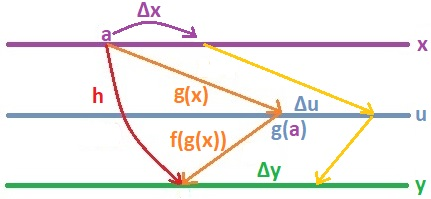
\includegraphics[scale=0.7]{img/intro-chain-rule-4.jpg}
\end{figure}

Entonces, la derivada de $h(x)$, que podemos denotar como $\frac{dy}{dx}$, será igual al límite de la razón entre el cambio en $y$ ($\Delta y$) y el cambio en $x$ ($\Delta x$), a medida que $\Delta x$ se acerca a cero.
\[\frac{dy}{dx} = \lim_{\Delta x \to 0} \frac{\Delta y}{\Delta x}\]
Ahora bien, como vemos en la imagen de arriba, el cambio en $y$ ocurre producto del cambio en $u$ y, este último, del cambio en $x$, puesto que $y$ está en función de $u$, y $u$ que está en función de $x$. Por lo tanto, el límite de la razón entre $\Delta y$ y $\Delta x$, a medida que $\Delta x \to 0$, será el producto del cambio de los límites, mientras $\Delta x \to 0$, de la razón entre el cambio en $y$ y el cambio en $u$ (porque $y$ está en función de $u$); y de la razón entre el cambio en $u$ y el cambio en $x$.
\[\lim_{\Delta x \to 0} \frac{\Delta y}{\Delta x} = \lim_{\Delta x \to 0} \left(\frac{\Delta y}{\Delta u} \cdot \frac{\Delta u}{\Delta x}\right)\]
Por consiguiente, la derivada de $h(x)$ o $\frac{dy}{dx}$ será igual a:
\[\frac{dy}{dx} = \lim_{\Delta x \to 0} \left(\frac{\Delta y}{\Delta u} \cdot \frac{\Delta u}{\Delta x}\right)\]
\[\frac{dy}{dx} = \lim_{\Delta x \to 0} \frac{\Delta y}{\Delta u} \cdot \lim_{\Delta x \to 0} \frac{\Delta u}{\Delta x}\]
Si volvemos a la última imagen de arriba, podemos apreciar que a medida que $\Delta x$ se acerca a una magnitud, en esa misma magnitud lo hace $\Delta u$. Por consiguiente, podemos decir que a medida que $\Delta x \to 0$, también $\Delta u \to 0$ y esta información la podemos agregar e la última fórmula que vimos.
\[\frac{dy}{dx} = \lim_{\Delta u \to 0} \frac{\Delta y}{\Delta u} \cdot \lim_{\Delta x \to 0} \frac{\Delta u}{\Delta x}\]
Por lo tanto, podemos decir que, en el lado izquierdo de la ecuación, el límite de la izquierda corresponde a la derivada de $y$ en función de $u$ y, la de la derecha es la derivada en $u$ en función de $x$:
\[\frac{dy}{dx} = \frac{dy}{du} \cdot \frac{du}{dx}\]
Y esto es valido a medida que las $\Delta u$ se cancelan, debido a que $\Delta x \to 0$.

Algo que no debemos olvidar es señalar en qué valor de $x$ estamos tomando las derivadas. Por facilidad, volvamos a ver el último esquema que dibujamos.

\newpage

\begin{figure}[hbt!]
\centering
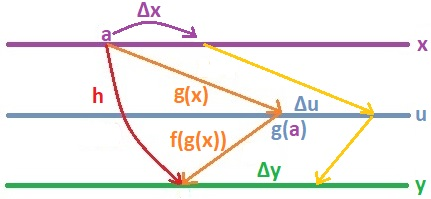
\includegraphics[scale=0.7]{img/intro-chain-rule-4.jpg}
\end{figure}

Como podemos observar, nuestro punto inicial es $x = a$, de manera que la derivada de $h(x)$, o $\frac{dy}{dx}$, está siendo tomada desde aquel valor. Esto implica que la derivada de $g(x)$, o $\frac{du}{dx}$, también tiene como punto inicial $x = a$. No obstante, el \textit{input} $f(x)$ proviene de $g(x)$ o, en otras palabras, de $u$. Por lo tanto, la derivada de $f(x)$, o $\frac{dy}{du}$ va a estar definida en $u = g(a)$. Es decir:
\[\diff{y}x[x = a] = \diff{y}u[u = g(a)] \cdot \diff{u}x[x = a]\]
En notación de Newton lo denotamos como:
\[h'(a) = f'(g(a)) \cdot g(a)\]
Esta corresponde, por lo tanto, a la fórmula de la \textbf{regla de la cadena}.




\subsection{Ejemplos Regla de la Cadena.}

Ahora, veamos el siguiente caso:
\[p(x) = cos^{3}(x)\]
La función $p(x)$ es una composición de funciones. Como recordaremos, éstas se expresan a partir de la forma:
\[(f \circ g)(x) = f(g(x))\]

\newpage

Donde:

\begin{itemize}
\item $g(x) \rightarrow$ Función de adentro.
\item $f(x) \rightarrow$ Función de afuera.
\end{itemize}

Sin embargo, al ver la función $p(x)$ podemos preguntarnos cómo sabemos cuál es la función que \underline{está adentro} (\textit{inner function}) y cuál es la que \underline{está afuera} (\textit{outer function}). Para resolver este asunto, debemos pensar y decidir \textbf{en qué orden calculamos $p(x)$}.

El \underline{orden} que podemos seguir para calcular la función $p(x)$, es el siguiente:

\begin{enumerate}
\item Calcular el $cos(x)$.
\item Elevar al cubo el resultado del $cos(x)$.
\end{enumerate}

Esto implica que:

\begin{enumerate}
\item Calcular el $cos(x)$ $\rightarrow$ Función de adentro.
\item Elevar al cubo el resultado del $cos(x)$ $\rightarrow$ Función de afuera.
\end{enumerate}

Por lo tanto, si queremos conocer la derivada de $g(x)$, debemos aplicar la \underline{regla de la cadena}.
\[p'(x) = (cos^{3}(x))' \cdot (cos(x))'\]
Por lo general, para trabajar de forma más ordenada en esta fórmula, la función de adentro suele ser asignada a una variable $u$, que es la variable intermedia que usamos anteriormente (pág. 37-38). En ese sentido, si la composición es $h(x) = f(g(x))$, entonces a partir de esta variable, $u = g(x)$. Por lo que:
\[h(x) = f(u)\]
Y su derivada pasará de:
\[h'(x) = f'(g(x)) \cdot g'(x)\]
A ser denotada como:
\[h'(x) = f'(u) \cdot g'(x)\]
Como dijimos, $cos(x)$ es la función de adentro de la composición $p(x)$, así que podemos asignarla a la variable intermedia $u$:
\[u = cos(x)\]
De manera que podemos expresarla como:
\[p(x) = u^{3}\]
Y, al querer calcular su derivada, aplicando la regla de la cadena quedará de esta forma:
\[p'(x) = (u^{3})' \cdot (u)'\]
\[p'(x) = 3u^{2} \cdot (u)'\]
Ahora, si reemplazamos a nuestras variables en función de $x$:
\[p'(x) = 3(cos(x))^{2} \cdot -sen(x)\]
Veamos otro ejemplo:
\[q(x) = cos(x^{3})\]
Otra vez, definimos cuál es la función de adentro cuál es la función de afuera. Si observamos bien, en dicha función, primero calculamos $x^{3}$ y, luego, calculamos el $cos(x)$ de dicho resultado. Es decir, al función de adentro es $x^{3}$ y la de afuera es $cos(x)$. Entonces, podemos asumir que nuestra variable intermedia es $x^{3}$:
\[u = x^{3}\]
Por lo que la función $q(x)$, será:
\[q(x) = cos(u)\]
Y, si calculamos su derivada aplicando la regla de la cadena:
\[q'(x) = (cos(u))' \cdot (x^{3})'\]
\[q'(x) = -sen(u) \cdot 3x^{2}\]
Si asignamos ambos factores en función de $x$, como lo eran originalmente:
\[q'(x) = -sen(x^{3}) \cdot 3x^{2}\]
Veamos ahora una función más compleja:
\[f(x) = \sqrt{x} \ tan(x^{2})\]
Si observamos bien la función $f(x)$, tiene varios elementos: es el producto entre una raíz cuadrada y una función tangente cuyo \textit{input} es el cuadrado de un valor. En ese sentido, si queremos calcular su derivada, bien podríamos preguntarnos por dónde partimos.

Comencemos por observar más en general la función $f(x)$. Así nos daremos cuenta que estamos multiplicando dos funciones. Por ejemplo, podemos decir que $g(x) = \sqrt{x}$ y que $h(x) = tan(x^{2})$. Por consiguiente, podemos denotar a $f(x)$ como:
\[f(x) = g(x) \cdot h(x)\]
En ese sentido, si queremos calcular la derivada de $f(x)$, podemos aplicar la \underline{regla del producto}:
\[f'(x) = (g(x) \cdot h(x))'\]
\[f'(x) = g(x) \cdot h'(x) + h(x) \cdot g'(x)\]
Calculemos, en primera instancia, las derivadas de ambas funciones. Partamos por $g(x)$:
\[g'(x) = (\sqrt{x})'\]
\[g'(x) = (x^{1/2})'\]
\[g'(x) = (x^{1/2})'\]
\[g'(x) = \frac{1}{2} \cdot (x^{-1/2})\]
Veamos cuál es la derivada de $h(x)$:
\[h'(x) = (tan(x^{2}))'\]
Como podemos observar, corresponde a una composición de funciones, en donde tenemos como función de adentro a $x^{2}$, mientras que la función de afuera es $tan(x)$. Por lo tanto, podemos designar como variable intermedia a $u = x^{2}$ y así podemos aplicar la \underline{regla de la cadena}:
\[h'(x) = (tan(u))'\]
\[h'(x) = (tan(u))' \cdot (u)'\]
\[h'(x) = \left(\frac{sen(u)}{cos(u)}\right)' \cdot (x^{2})'\]
Como vemos, para la $tan(x)$ podemos usar la \underline{regla del cuociente}:
\[h'(x) = \frac{cos(u) \cdot (sen(u))' - sen(u) \cdot (cos(u)')}{cos^{2}(u)} \cdot 2x\]
\[h'(x) = \frac{cos(u) \cdot cos(u) - sen(u) \cdot (-sen(u))}{cos^{2}(u)} \cdot 2x\]
\[h'(x) = \frac{cos^{2}(u) + sen^{2}(u)}{cos^{2}(u)} \cdot 2x\]
\[h'(x) = \frac{1}{cos^{2}(u)} \cdot 2x\]
\[h'(x) = sec^{2}(u) \cdot 2x\]
Como sabemos que $u = x^{2}$, entonces:
\[h'(x) = sec^{2}(x^{2}) \cdot 2x\]
Ahora volvamos a la derivada de $f(x)$:
\[f'(x) = g(x) \cdot h'(x) + h(x) \cdot g'(x)\]
Reemplacemos los valores de las funciones y sus derivadas, por los originales:
\[f'(x) = \sqrt{x} \cdot (sec^{2}(x^{2}) \cdot 2x) + tan(x^{2}) \cdot \frac{1}{2} \cdot (x^{-1/2})\]
\[f'(x) = x^{1/2} \cdot (2x \cdot sec^{2}(x^{2})) + tan(x^{2}) \cdot \frac{1}{2x^{1/2}}\]
\[f'(x) = 2x^{3/2} \cdot sec^{2}(x^{2}) + \frac{tan(x^{2})}{2x^{1/2}}\]
Continuemos con el siguiente ejemplo:
\[g(x) = \sqrt{x \ tan(x)}\]
Es bastante similar a la anterior función $f(x)$, salvo que el cálculo de sus derivadas, es distinto.

Si observamos bien la función $g(x)$, si queremos calcular un \textit{output} de ella, lo último que calcularemos será la raíz cuadrada de toda aquella expresión. Como es una función compuesta, podemos decir que $x \ tan(x)$, es la función de adentro; mientras que la $\sqrt{x}$, es la función de afuera. De manera que:
\[g(x) = \sqrt{u} \quad \mathrm{donde} \quad u = x \ tan(x)\]
Por lo tanto, para calcular la derivada de $g(x)$, podemos aplicar la regla de la cadena:
\[g'(x) = (\sqrt{u})' \cdot (u)'\]
\[g'(x) = (u^{1/2})' \cdot (x \cdot tan(x))'\]
\[g'(x) = \frac{1}{2} \cdot u^{-1/2} \cdot (x \cdot (tan(x))' + (x)' \cdot tan(x))\]
\[g'(x) = \frac{1}{2} \cdot (x \cdot tan(x))^{-1/2} \cdot (x \cdot sec^{2}(x) + tan(x))\]
Revisemos un último ejemplo sobre la regla de la cadena: 

Busque \underline{dos valores} para $\Theta$, tal que:
\[\frac{d}{d \Theta} (cos^{2}(\Theta^{4})) = 0\]
La función $cos^{2}(\Theta^{4})$ también podemos leerla como $(cos(\Theta^{4}))^{2}$. En ese sentido, y a diferencia de los ejemplos anteriores, acá tenemos una función que está compuesta de otras \underline{dos} funciones (anteriormente era solo por una). Es decir, tenemos dos funciones internas o intermedias.

Si lo vemos en términos de menor a mayor ``profundidad'', estas funciones serían las siguientes:

\begin{itemize}
\item Función externa $\rightarrow$ $(cos(\Theta^{4}))^{2}$.
\item Primera función interna $\rightarrow$ $cos(\Theta^{4})$.
\item Segunda función interna $\rightarrow$ $\Theta^{4}$
\end{itemize}

Asignémosle una variable a cada función:

\begin{itemize}
\item $y = (cos(\Theta^{4}))^{2}$
\item $x = cos(\Theta^{4})$
\item $w = \Theta^{4}$
\end{itemize}

Como es $y$ es una función compuesta (en este caso por dos funciones), podemos aplicar la regla de la cadena para derivarla, la que lucirá de la siguiente manera:
\[\frac{dy}{d \Theta} = \frac{dy}{dx} \cdot \frac{dx}{dw} \cdot \frac{dw}{d \Theta}\]
Es decir:
\[((cos(\Theta^{4}))^{2})' = (x^{2})' \cdot (cos(w))' \cdot (\Theta^{4})'\]
\[((cos(\Theta^{4}))^{2})' = 2x \cdot (-sen(w)) \cdot 4\Theta^{3}\]
\[((cos(\Theta^{4}))^{2})' = 8x \cdot (-sen(w)) \cdot \Theta^{3}\]
Si reemplazamos por los valores originales de $x$ y de $w$:
\[((cos(\Theta^{4}))^{2})' = 8cos(\Theta^{4}) \cdot (-sen(\Theta^{4})) \cdot \Theta^{3}\]
\[((cos(\Theta^{4}))^{2})' = -8\Theta^{3} \cdot cos(\Theta^{4}) \cdot sen(\Theta^{4})\]
En este ejercicio nos preguntan por dos valores de $\Theta$ en donde la derivada que vemos arriba, sea igual a cero. Si vemos bien la fórmula, \underline{un caso es que $\Theta = 0$}. Es decir:
\[((cos(0^{4}))^{2})' = -8 \cdot 0^{3} \cdot cos(0^{4}) \cdot sen(0^{4})\]
\[((cos(0^{4}))^{2})' = 0 \cdot cos(0^{4}) \cdot sen(0^{4})\]
\[((cos(0^{4}))^{2})' = 0\]
El segundo caso puede ser a partir de la función $sen(\Theta)$ o $cos(\Theta)$. Como recordaremos, ambas funciones son periodicas y, para ciertos valores de $\Theta$, serán iguales a cero. Si una de ellas se iguala a cero, entonces el valor de esta derivada también resultará en dicho valor.

Usemos como \underline{segundo caso} a $\Theta = \pi/2$. Cuando alcanza dicho valor, entonces $cos(\Theta)$ se iguala a cero (i.e., $cos(\pi/2) = 0$). Llevémoslo a la derivada de este ejemplo.
\[((cos(\Theta^{4}))^{2})' = -8 \cdot \left(\frac{\pi}{2}\right)^{3} \cdot cos\left(\left(\frac{\pi}{2}\right)^{4}\right) \cdot sen\left(\left(\frac{\pi}{2}\right)^{4}\right)\]
\[((cos(\Theta^{4}))^{2})' = -8 \cdot \left(\frac{\pi}{2}\right)^{3} \cdot 0 \cdot sen\left(\left(\frac{\pi}{2}\right)^{4}\right)\]
\[((cos(\Theta^{4}))^{2})' = 0\]




\subsection{Derivación Implícita.}

Hasta ahora, hemos diferenciado ecuaciones que cumplen con el requisito para ser catalogadas como funciones: cada valor de entrada (\textit{input}) tiene un único valor de salida (\textit{output}). Pero ¿qué ocurre si una ecuación no es una función? ¿Cómo podemos derivarla/diferenciarla?

Por ejemplo, veamos el caso de la ecuación de la circunferencia, con su centro $C(h, \ k)$ en el origen\footnote{Si no fuera en el origen, su ecuación sería: $(x - h)^{2} + (y - k)^{2} = r^{2}$.}.
\[x^{2} + y^{2} = r^{2}\]
En particular, digamos que tiene un radio $r = 5$.
\[x^{2}+y^{2} = 25\]
Si trazamos la curva de esta ecuación y realizamos la prueba de la línea recta en $x = -3$, para ver si cumple con ser una función, podremos observar que fracasa en alcanzar este requisito.

\begin{figure}[hbt!]
\centering
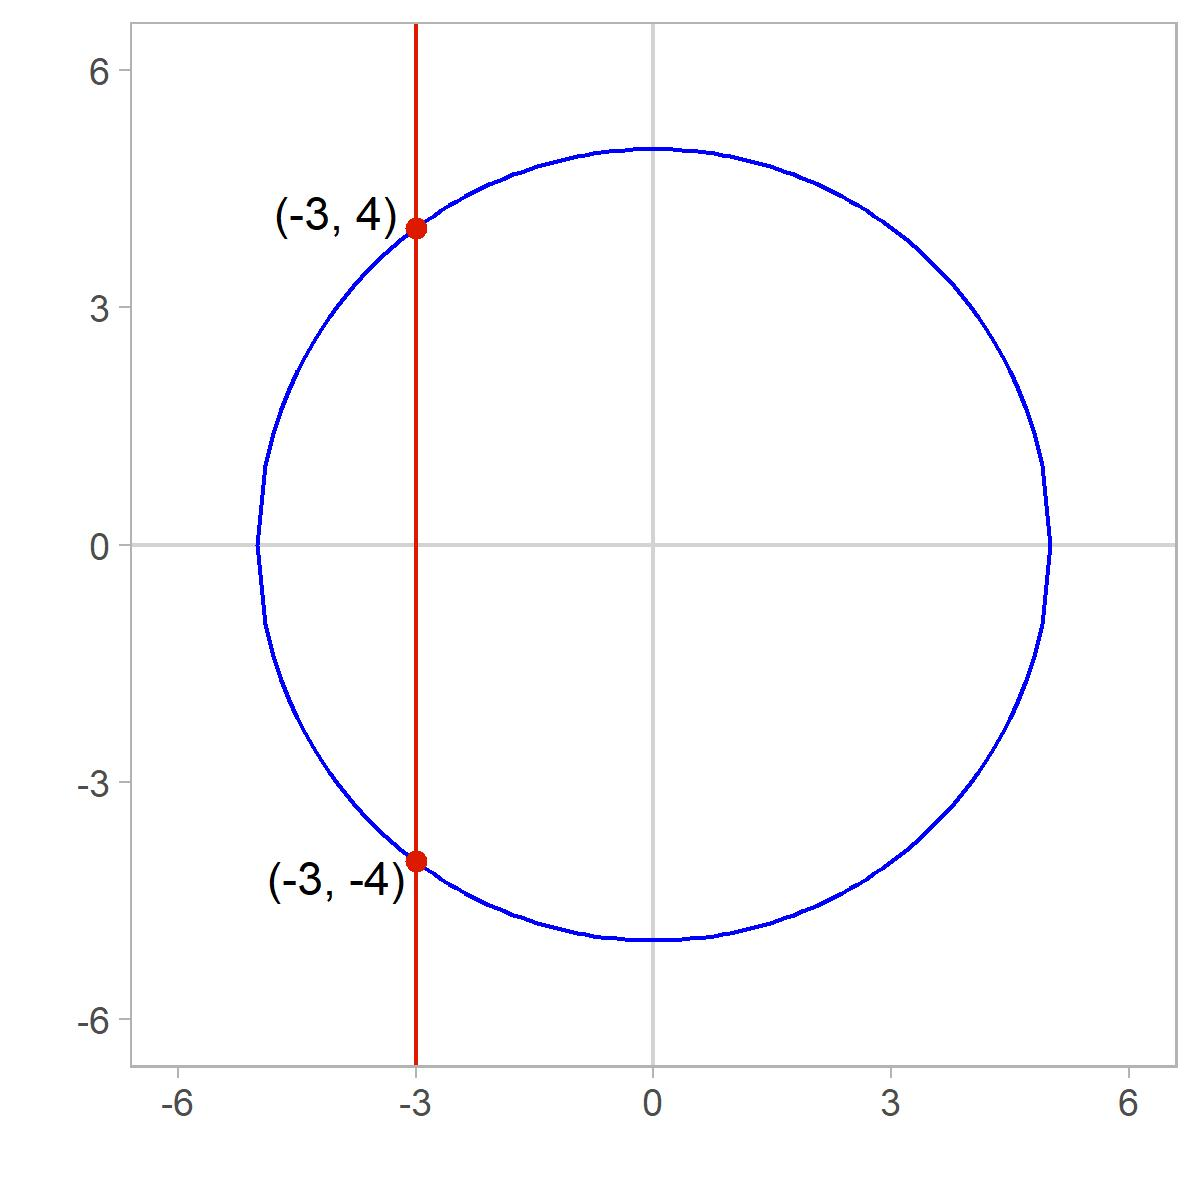
\includegraphics[scale=0.7]{img/implicit_diff.jpg}
\end{figure}

De todas maneras, diferenciemos esta ecuación. Partamos por buscar una \textbf{fórmula explícita} para $x^{2}+y^{2} = 25$ para $y$ en términos de $x$.
\[x^{2}+y^{2} = 25\]
\[y^{2} = 25 - x^{2}\]
\[y = \pm \sqrt{25 - x^{2}}\]
Como vemos, obtuvimos dos fórmulas, que en la gráfica una representa a la mitad de arriba (positiva) y la otra a la mitad de abajo (negativa):
\[y_{1} = \sqrt{25 - x^{2}} \quad \mathrm{y} \quad y_{2} = -\sqrt{25 - x^{2}}\]

\newpage

\begin{figure}[hbt!]
\centering
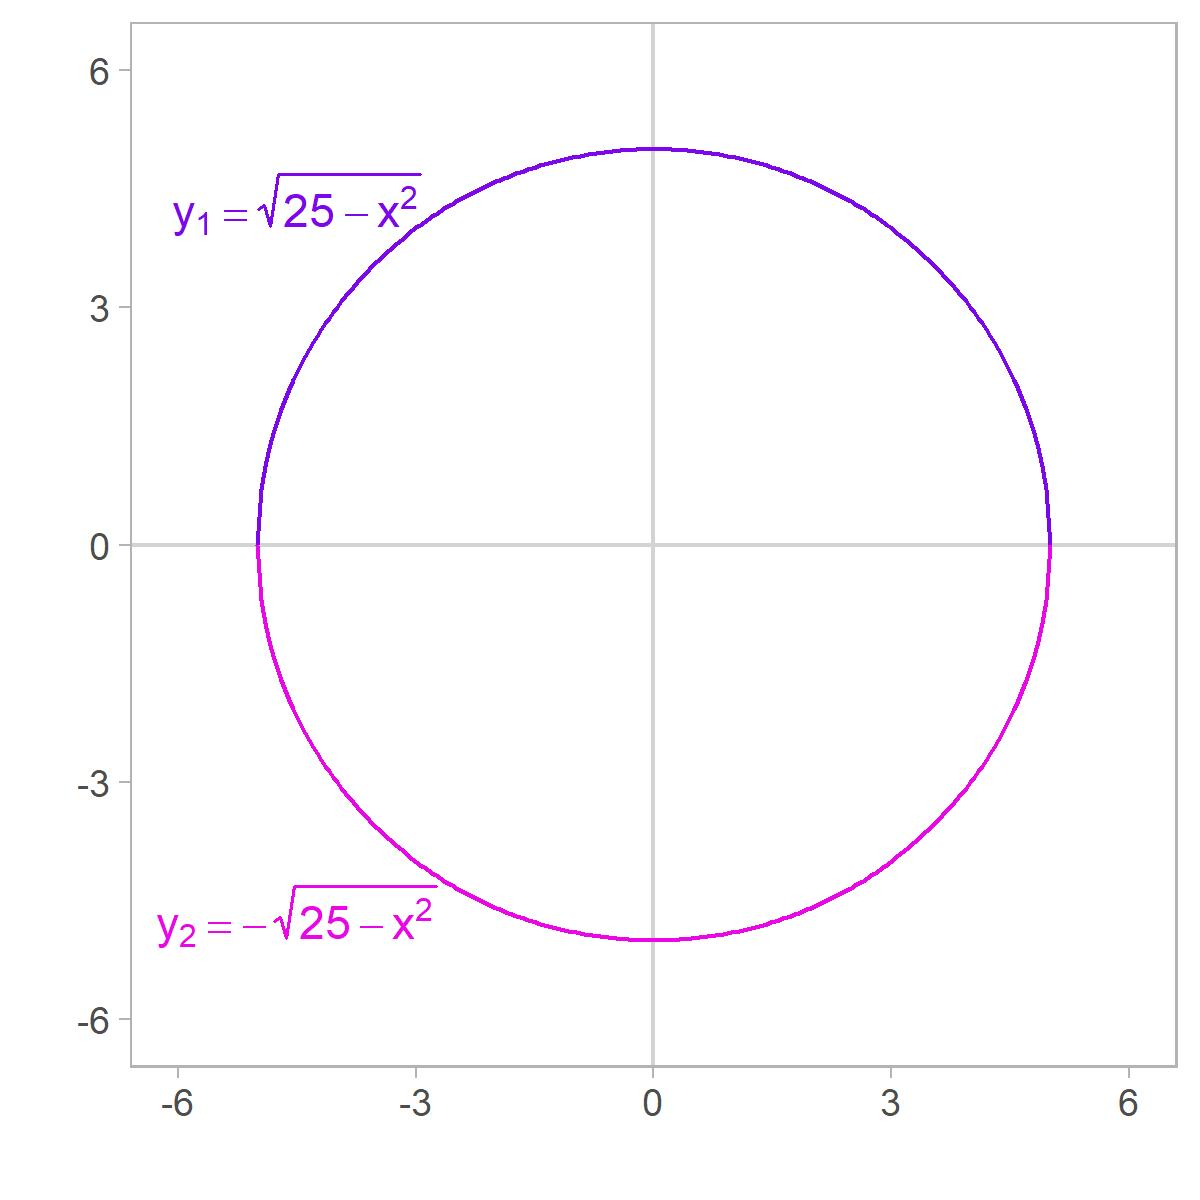
\includegraphics[scale=0.7]{img/implicit_diff_2.jpg}
\end{figure}

Calculemos la derivada de ambas ecuaciones. Comencemos con la primera.
\[\frac{dy_{1}}{dx} = (\sqrt{25 - x^{2}})'\]
\[\frac{dy_{1}}{dx} = (\sqrt{u})' \cdot (25 - x^{2})'\]
\[\frac{dy_{1}}{dx} = \frac{1}{2}u^{-1/2} \cdot (-2x)\]
\[\frac{dy_{1}}{dx} = -u^{-1/2} \cdot x\]
\[\frac{dy_{1}}{dx} = -(25 - x^{2})^{-1/2} \cdot x\]
Sigamos con la segunda ecuación.
\[\frac{dy_{2}}{dx} = (-\sqrt{25 - x^{2}})'\]
\[\frac{dy_{2}}{dx} = (-1 \cdot \sqrt{25 - x^{2}})'\]
\[\frac{dy_{2}}{dx} = (-1)' \cdot \sqrt{25 - x^{2}} + (\sqrt{25 - x^{2}})' \cdot -1\]
\[\frac{dy_{2}}{dx} = 0 + -(\sqrt{25 - x^{2}})'\]
\[\frac{dy_{2}}{dx} = -[(\sqrt{u})' \cdot (25 - x^{2})']\]
\[\frac{dy_{2}}{dx} = -\left[\frac{1}{2} (u)^{-1/2} \cdot (0 - 2x)\right]\]
\[\frac{dy_{2}}{dx} = -\left[\frac{1}{2} (u)^{-1/2} \cdot -2x\right]\]
\[\frac{dy_{2}}{dx} = -[-(u)^{-1/2} \cdot x]\]
\[\frac{dy_{2}}{dx} = u^{-1/2} \cdot x\]
\[\frac{dy_{2}}{dx} = (25 - x^{2})^{-1/2} \cdot x\]
Ahora bien, esta forma de encontrar tanto las fórmulas en función de $x$ como sus derivadas de la ecuación de la circunferencia, fue un poco desordenada. No obstante, podemos hacer el mismo trabajo, pero de una manera \textbf{implícita}.

Volvamos a la ecuación original.
\[x^{2} + y^{2} = 25\]
En esta ocasión vamos a pensar \textbf{implícitamente} a $y$ como una función de $x$, pero no buscaremos una ecuación explícita. Más bien, la pensaremos como una \textbf{ecuación de funciones}:
\[x^{2} + y(x)^{2} = 25\]
Es decir, la parte izquierda de la ecuación, $x^{2} + y(x)^{2}$, la asumimos como una función de $x$ en donde, para cualquier valor de entrada, va a ser igual a $25$. En otras palabras, será una función constante de $x$.

Lo anterior es exactamente de lo que se trata estar en el círculo que se forma a partir de la ecuación $x^{2} + y^{2} = 25$. Si tenemos un valor en $x$, entonces $y(x)$ está determinado, por lo que $x^{2} + y(x)^{2} = 25$.

Por consiguiente, si ambos lados de la ecuación $x^{2} + y(x)^{2} = 25$, son \textbf{iguales como funciones de $x$}, entonces podemos diferenciarlas con respecto a $x$. Y, al hacerlo, ambos lados seguirán siendo iguales:
\[\frac{d}{dx} (x^{2} + y(x)^{2}) = \frac{d}{dx} (25)\]
\[\frac{d}{dx}(x^{2}) + \frac{d}{dx}(y(x))^{2} = 0\]
\[2x + \left(\frac{d}{dx}(y(x)^{2}) \cdot \frac{d}{dx}(y(x)) \cdot \frac{d}{dx}(x)\right) = 0\]
\[2x + \left(2y(x) \cdot \frac{dy}{dx} \cdot 1\right) = 0\]
\[2x + 2y(x) \cdot \frac{dy}{dx} = 0\]
Ahora tenemos una ecuación, así que resolvémosla para $\frac{dy}{dx}$:
\[2y(x) \cdot \frac{dy}{dx} = -2x\]
\[\frac{1}{2y} \cdot 2y(x) \cdot \frac{dy}{dx} = \frac{1}{2y} \cdot -2x\]
\[\frac{dy}{dx} = -\left(\frac{x}{y}\right)\]
Como podemos observar, la fórmula de arriba para $\frac{dy}{dx}$ involucra tanto a $y$ como a $x$. Veamos por qué la dejamos de está manera.

La ecuación original de la circunferencia con la que estamos trabajando, $x^{2} + y^{2} = 25$, se aplica a \textbf{todos los puntos que la conforman}. Es decir, tanto a la mitad de arriba como a la mitad de abajo. En ese sentido, la \textbf{fórmula de la derivada} que encontramos de manera \textbf{implícita}, $\frac{dy}{dx} = -\left(\frac{x}{y}\right)$, también \textbf{se aplica en ambas partes de su gráfica} o en todos sus puntos.

Revisemos algunos casos.

Por ejemplo, si $y = 0$, entonces la derivada será un valor indeterminado. Esto ocurre cuando $x = \pm 5$, en donde las pendientes de las rectas tangentes son valores infinitos y, por consiguiente, sus gráficas son líneas rectas verticales.

\newpage

\begin{figure}[hbt!]
\centering
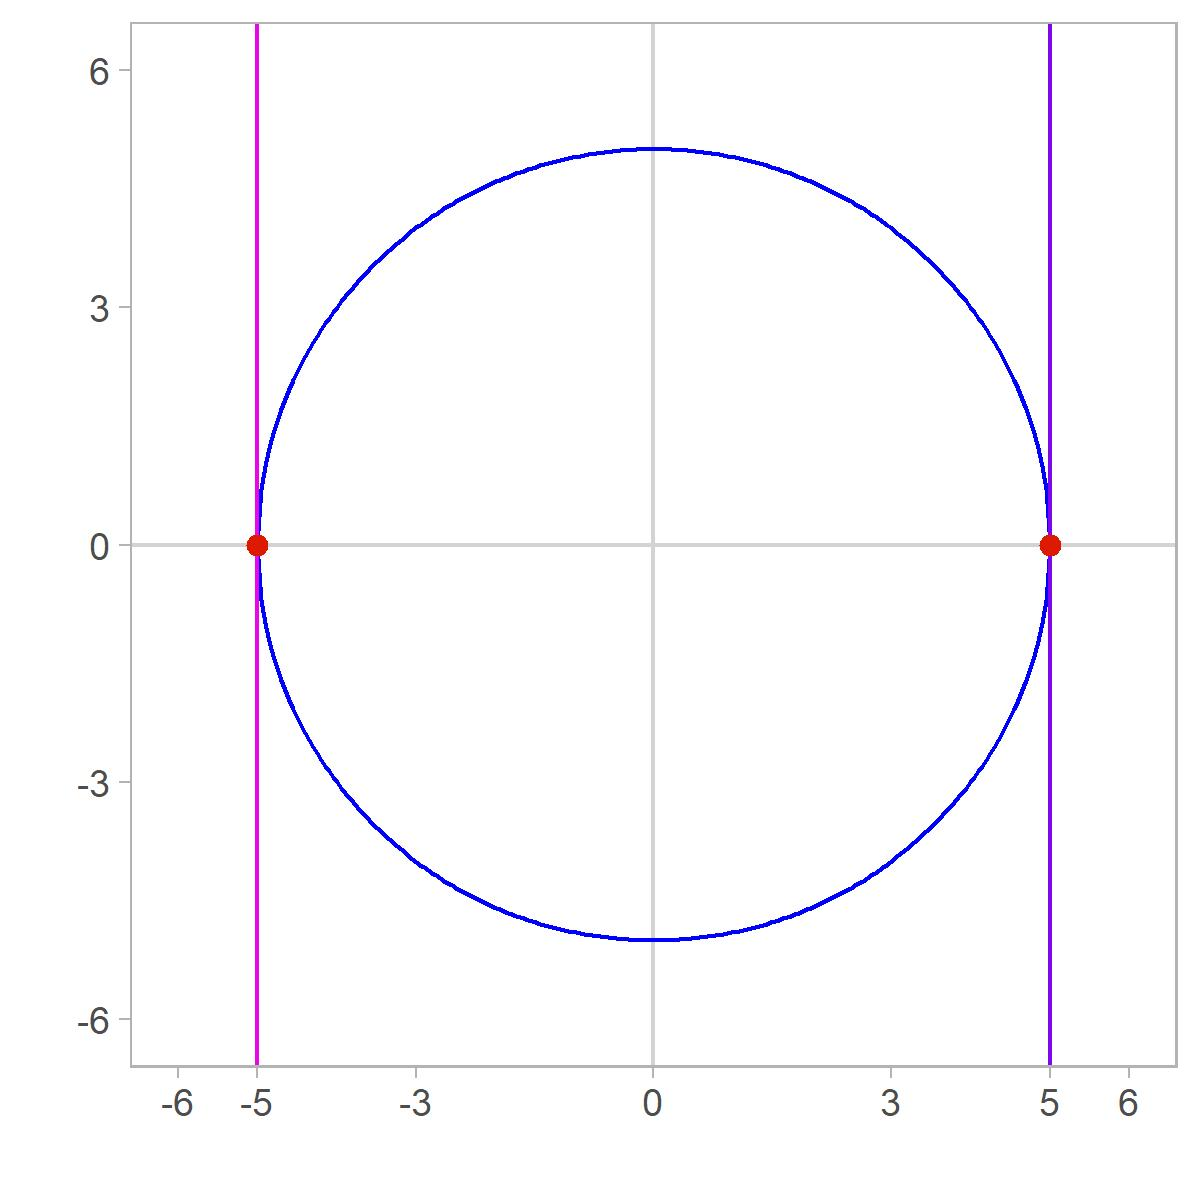
\includegraphics[scale=0.7]{img/implicit_diff_3.jpg}
\end{figure}

Por otra parte, cuando $x = 0$, la derivada se iguala a cero:
\[\frac{dy}{dx} = - \frac{0}{y}\]
\[\frac{dy}{dx} = 0\]
En este caso, es posible encontrar dos valores de salida: $y = \pm 5$. Como veremos a continuación, justamente las pendientes de las líneas tangentes que se forman en los puntos $(0, \ 5)$ y $(0, \ -5)$, son iguales a cero o, en otras palabras, líneas rectas horizontales.

\newpage

\begin{figure}[hbt!]
\centering
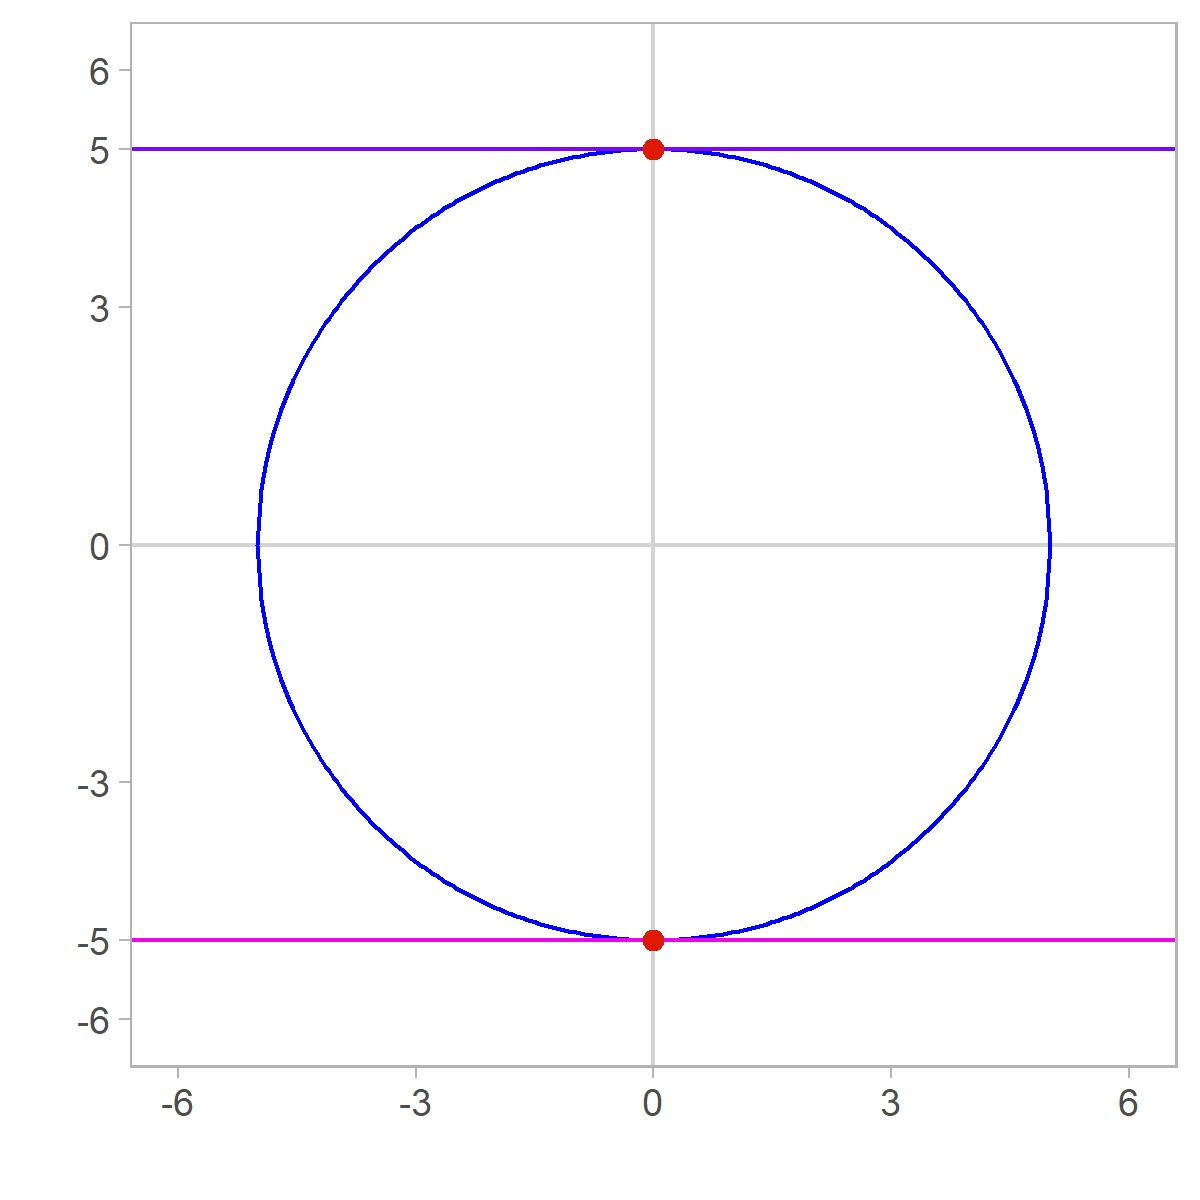
\includegraphics[scale=0.7]{img/implicit_diff_4.jpg}
\end{figure}

También podemos ver el comportamiento de las líneas tangentes según el cuadrante en donde se ubique un punto que conforma a la circunferencia $x^{2} + y^{2} = 25$. Por ejemplo, todas las derivadas de los puntos que están en el segundo cuadrante (sin considerar a $x = 0$ y a $y = 0$), serán de signo positivo, puesto que la fracción será negativa y, por tanto, estaremos multiplicándola con el valor negativo de afuera. Veamos el caso del punto $(-3, \ 4)$.
\[\frac{dy}{dx} = -\left(\frac{x}{y}\right)\]
\[\frac{dy}{dx} = -\left(\frac{-3}{4}\right)\]
\[\frac{dy}{dx} = -(-0.75)\]
\[\frac{dy}{dx} = 0.75\]
Si graficamos la recta tangente en dicho punto, veremos que se inclinará en sentido positivo:

\newpage

\begin{figure}[hbt!]
\centering
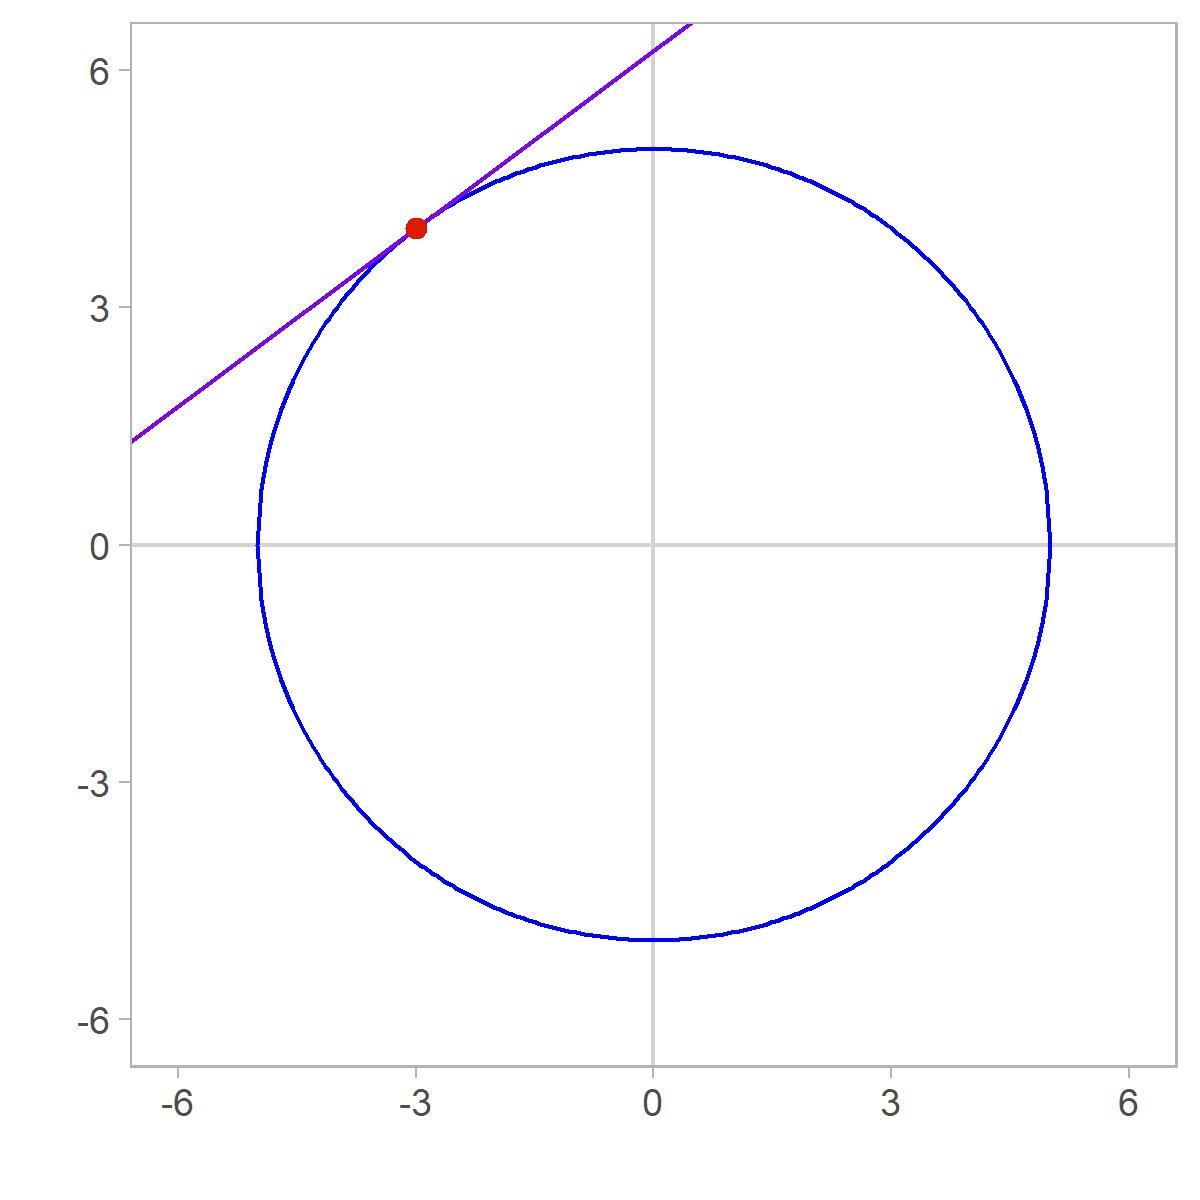
\includegraphics[scale=0.7]{img/implicit_diff_5.jpg}
\end{figure}

1) \underline{Demostración de la Regla de la Potencia para Exponentes Racionales}.

Un caso en donde podemos aplicar lo que aprendimos sobre derivación implícita, es en la demostración la regla de la potencia cuando su exponente es un número racional.

Recordemos que la regla de la potencia se define de la siguiente manera:
\[\frac{d}{dx} x^{r} = r \cdot x^{1-r}\]
Si bien hemos usado esta fórmula asumiendo que $r \in \mathbb{R}$, hemos probado que es verdadera solo para valores de $r$ que son números enteros (i.e, conjunto $\mathbb{Z}$). Ahora lo haremos para números racionales (conjunto $\mathbb{Q}$). En particular, diremos que:
\[r = \frac{m}{n} \quad \mathrm{donde} \quad m \neq 0, \ n \neq 0 \ \mathrm{y} \ n \neq 1\]
Por lo que la regla de la potencia se definirá de este modo:
\[\frac{d}{dx} x^{m/n} = \frac{m}{n} \cdot x^{(m/n)-1}\]
Para demostrarla, la derivaremos implícitamente porque nos hace la tarea mucho más fácil que si la hiciéramos de forma explícita.

Entonces, para derivarla implícitamente, diremos que $x^{m/n}$ es una función de $y(x)$. Es decir:
\[y = x^{m/n}\]
Algo que debemos tener en cuenta es que una demostración la podemos realizar solo a partir de lo que probamos en el pasado. Y, como dijimos, en la regla de la potencia lo hemos hecho para exponentes que son números enteros. Por lo tanto, lo que podemos hacer es elevar a un número $n \in \mathbb{Z}$:
\[y^{n} = (x^{m/n})^{n}\]
\[y^{n} = x^{(m/n) \cdot n}\]
\[y^{n} = x^{m}\]
Ahora tenemos una función que podemos derivar implícitamente y en ambos lados de la ecuación:
\[\frac{d}{dx} y^{n} = \frac{d}{dx} x^{m}\]
Apliquemos la regla de la cadena para el lado izquierdo:
\[\frac{d}{dy} (y)^{n} \cdot \frac{d}{dx} y = m \cdot x^{m-1}\]
\[n \cdot y^{n-1} \cdot \frac{d}{dx} y = m \cdot x^{m-1}\]
Definamos esta ecuación para $\frac{dy}{dx}$:
\[\frac{dy}{dx} = \frac{m \cdot x^{m-1}}{n \cdot y^{n-1}}\]
Anteriormente definimos que $y = x^{m/n}$, por lo tanto:
\[\frac{dy}{dx} = \frac{m \cdot x^{m-1}}{n \cdot (x^{m/n})^{n-1}}\]
\[\frac{dy}{dx} = \frac{m \cdot x^{m-1}}{n \cdot x^{(mn-m)/n}}\]
\[\frac{dy}{dx} = \frac{m}{n} \cdot x^{(m-1) - [(mn-m)/n]}\]
\[\frac{dy}{dx} = \frac{m}{n} \cdot x^{(-n + m)/n}\]
Esto es lo mismo que:
\[\frac{dy}{dx} = \frac{m}{n} \cdot x^{-1 + (m/n)}\]
\[\frac{dy}{dx} = \frac{m}{n} \cdot x^{(m/n) - 1}\]
Como vemos, hemos demostrado la fórmula de la regla de la potencia para exponentes con números racionales, derivando implícitamente.

Ahora revisemos la siguiente ecuación:
\[x^{4} - 3x^{2} + y^{4} + y^{2} + 2x^{2}y^{2} = 0\]
De la cual se forma la siguiente curva\footnote{No pude graficarla en R, pero espero en algún momento lograr esa hazaña. De todos modos, las soluciones a esta ecuación es posible encontrarlas \href{https://es.symbolab.com/solver/functions-calculator/simplificar\%20x\%5E\%7B4\%7D-\%203x\%5E\%7B2\%7D\%2B\%20y\%5E\%7B4\%7D\%2B\%20y\%5E\%7B2\%7D\%2B2x\%5E\%7B2\%7Dy\%5E\%7B2\%7D\%3D\%200}{acá}.}:

\begin{figure}[hbt!]
\centering
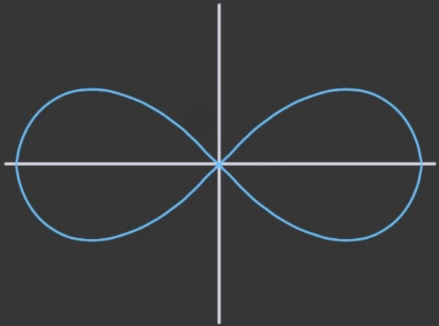
\includegraphics[scale=0.7]{img/implicit_diff_6.jpg}
\end{figure}

Y buscaremos responder las siguientes preguntas:

\begin{enumerate}
\item ¿Cuál es la pendiente de la línea tangente en $(x, \ y) = \left(\frac{1}{\sqrt{2}}, \ \frac{1}{\sqrt{2}}\right)$?
\item ¿En qué puntos esta función tiene una línea tangente horizontal?
\end{enumerate}

Como podemos apreciar en las preguntas, en ambas necesitamos tener conocimiento de la derivada de esta ecuación (i.e., la pendiente de la línea tangente) para todos sus puntos.

Para ello, una forma sería igualar en $y$ la ecuación (en otras palabras, buscarla explícitamente) para luego derivarla, pero eso sería muy tedioso (ver enlace de pie de página 3, pág. 56). Es por ello que la mejor opción es derivarla implícitamente, como lo ya lo hicimos en los ejemplos anteriores.
\[\frac{d}{dx}(x^{4} - 3x^{2} + y^{4} + y^{2} + 2x^{2}y^{2}) = \frac{d}{dx} \ 0\]
\[\frac{d}{dx} (x^{4}) - \frac{d}{dx}(3x^{2}) + \frac{d}{dx} (y^{4}) + \frac{d}{dx}(y^{2}) + \frac{d}{dx}(2x^{2}y^{2}) = 0\]
\[4x^{3} - 6x + \left(\frac{d}{dy} (y^{4}) \cdot \frac{d}{dx} (y)\right) + \left(\frac{d}{dy} (y^{2}) \cdot \frac{d}{dx} (y)\right) + \frac{d}{dx}(2x^{2}y^{2}) = 0\]
\[4x^{3} - 6x + \left(4y^{3} \cdot \frac{d}{dx} (y)\right) + \left(2y \cdot \frac{d}{dx} (y)\right) + \frac{d}{dx}(2x^{2}y^{2}) = 0\]
\[4x^{3} - 6x + (4y^{3} + 2y) \cdot \frac{d}{dx} (y) + \frac{d}{dx}(2x^{2}y^{2}) = 0\]
Por un tema de legibilidad, resolveremos de forma separada la última derivada de la izquierda, $\frac{d}{dx}(2x^{2}y^{2})$.
\[\frac{d}{dx}(2x^{2}y^{2}) = \frac{d}{dx}(2x^{2}) \cdot y^{2} + \frac{d}{dx}(y^{2}) \cdot 2x^{2}\]
\[\frac{d}{dx}(2x^{2}y^{2}) = 4x \cdot y^{2} + \left(\frac{d}{dy}(y^{2}) \cdot \frac{d}{dx} (y)\right) \cdot 2x^{2}\]
\[\frac{d}{dx}(2x^{2}y^{2}) = 4x \cdot y^{2} + 2y \cdot \frac{d}{dx} (y) \cdot 2x^{2}\]
\[\frac{d}{dx}(2x^{2}y^{2}) = 4xy^{2} + 4x^{2}y \cdot \frac{d}{dx} (y)\]
Reemplacemos este valor en la ecuación original de la derivada:
\[4x^{3} - 6x + (4y^{3} + 2y) \cdot \frac{d}{dx} (y) + 4xy^{2} + 4x^{2}y \cdot \frac{d}{dx}(y) = 0\]
\[4x^{3} - 6x + (4y^{3} + 2y + 4x^{2}y) \cdot \frac{d}{dx} (y) + 4xy^{2} = 0\]
Ahora resolvamos la ecuación para $\frac{dy}{dx}$:
\[(4y^{3} + 2y + 4x^{2}y) \cdot \frac{d}{dx} (y) = -4x^{3} + 6x - 4xy^{2}\]
\[\frac{d}{dx} (y) = \frac{-4x^{3} + 6x - 4xy^{2}}{4y^{3} + 2y + 4x^{2}y}\]
\[\frac{d}{dx} (y) = \frac{-2x \cdot(2x^{2} - 3 + 2y^{2})}{2y\cdot(2y^{2} + 1 + 2x^{2})}\]
\[\frac{d}{dx} (y) = -\frac{x}{y} \cdot \frac{(2x^{2} - 3 + 2y^{2})}{(2y^{2} + 1 + 2x^{2})}\]
Ahora que tenemos la derivada para todos los puntos, podemos responder las dos preguntas planteadas al inicio de este ejemplo (pág. 56).

En primer lugar, nos preguntan por la pendiente en el punto $\left(\frac{1}{\sqrt{2}}, \ \frac{1}{\sqrt{2}}\right)$, cuyas coordenadas podemos usar en la ecuación que acabamos de encontrar:
\[\diff{y}x[(\frac{1}{\sqrt{2}}, \ \frac{1}{\sqrt{2}})] = -\frac{1/\sqrt{2}}{1/\sqrt{2}} \cdot \frac{(2 \cdot (1/\sqrt{2})^{2} - 3 + 2 \cdot (1/\sqrt{2})^{2})}{(2 \cdot (1/\sqrt{2})^{2} + 1 + 2 \cdot (1/\sqrt{2})^{2})}\]
\[\diff{y}x[(\frac{1}{\sqrt{2}}, \ \frac{1}{\sqrt{2}})] = - \frac{(1 - 3 + 1)}{(1 + 1 + 1)}\]
\[\diff{y}x[(\frac{1}{\sqrt{2}}, \ \frac{1}{\sqrt{2}})] = - \left(\frac{-1}{3}\right) = \frac{1}{3}\]
Luego, nos preguntan por los puntos de la ecuación en donde la línea tangente es horizontal o, en otras palabras, en qué ubicación la derivada es igual a cero.
\[\frac{d}{dx} (y) = 0\]
Si vemos la fórmula de la derivada de este ejemplo, podemos percatarnos que hay dos formas de obtener dicho resultado. La primera es que $x = 0$, de manera que:
\[- \frac{x}{y} = - \frac{0}{y} = 0\]
Sin embargo, si observamos la curva de la ecuación de este ejemplo (pág. 56), nos daremos cuenta que en $x = 0$ no se forma una línea tangente horizontal y para ninguno de sus dos lados. Por lo tanto, descartamos esta opción.

La otra forma en que $\frac{d}{dx} (y) = 0$, es que la expresión $(2x^{2} - 3 + 2y^{2}) = 0$. Es decir:
\[\frac{(2x^{2} - 3 + 2y^{2})}{(2y^{2} + 1 + 2x^{2})} = \frac{0}{(2y^{2} + 1 + 2x^{2})} = 0\]
Y si despejamos aquella expresión para $x$ e $y$, nos encontraremos con una ecuación de la circunferencia de radio $r = \sqrt{\frac{3}{2}}$ y centrada en el origen:
\[2x^{2} - 3 + 2y^{2} = 0\]
\[2x^{2} + 2y^{2} = 3\]
\[2 \cdot (x^{2} + y^{2}) = 3\]
\[x^{2} + y^{2} = \frac{3}{2}\]
Esto quiere decir que si graficamos esta circunferencia en el gráfico de la ecuación de este ejemplo, podremos observar todos los puntos en donde $\frac{d}{dx} (y) = 0$, que corresponderán a aquellos en donde ambas gráficas se intersectan.

\begin{figure}[hbt!]
\centering
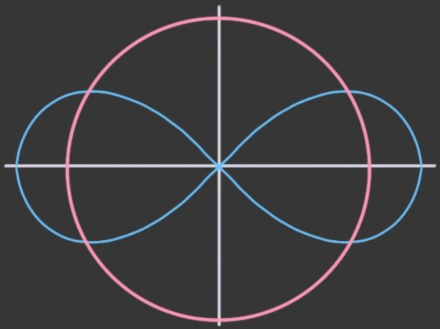
\includegraphics[scale=0.7]{img/implicit_diff_7.jpg}
\end{figure}

\newpage

Veamos en qué puntos aquella circunferencia intersecta a la gráfica de la ecuación de este ejemplo. Primero, despejemos la ecuación de la circunferencia en $x^{2}$:
\[x^{2} + y^{2} = \frac{3}{2}\]
\[x^{2} = \frac{3}{2} - y^{2}\]
Luego, usemos este valor de $x^{2}$ y reemplacémoslo en la ecuación de este ejemplo, para ver en qué puntos se intersectan ambas ecuaciones.
\[x^{4} - 3x^{2} + y^{4} + y^{2} + 2x^{2}y^{2} = 0\]
\[x^{2} \cdot x^{2} - 3x^{2} + y^{4} + y^{2} + 2x^{2}y^{2} = 0\]
\[\left(\frac{3}{2} - y^{2}\right) \cdot \left(\frac{3}{2} - y^{2}\right) - 3 \cdot \left(\frac{3}{2} - y^{2}\right) + y^{4} + y^{2} + 2 \cdot \left(\frac{3}{2} - y^{2}\right) \cdot y^{2} = 0\]
\[\left(\frac{3}{2} - y^{2}\right)^{2} - 3 \cdot \left(\frac{3}{2} - y^{2}\right) + y^{4} + y^{2} + 2 \cdot \left(\frac{3}{2} - y^{2}\right) \cdot y^{2} = 0\]
\[\frac{9}{4} - 3y^{2} + y^{4} - \frac{9}{2} + 3y^{2} + y^{4} + y^{2} + 3y^{2} - 2y^{4} = 0\]
\[- \frac{9}{4} + 4y^{2} = 0\]
\[4y^{2} = \frac{9}{4}\]
\[y^{2} = \frac{9}{16}\]
\[y = \pm \sqrt{\frac{9}{16}} = \pm \frac{3}{4}\]
El valor $y$ que acabamos de obtener, podemos usarlo en la ecuación de la circunferencia para encontrar a $x$:
\[x^{2} = \frac{3}{2} - y^{2}\]
\[x^{2} = \frac{3}{2} - \frac{9}{16}\]
\[x^{2} = \frac{15}{16}\]
\[x = \pm \sqrt{\frac{15}{16}} = \pm \frac{\sqrt{15}}{4}\]
Por lo tanto, los puntos en donde $\frac{d}{dx} (y) = 0$, son los siguientes:
\[\left(\frac{\sqrt{15}}{4}, \ \frac{3}{4}\right), \ \left(-\frac{\sqrt{15}}{4}, \ \frac{3}{4}\right), \ \left(-\frac{\sqrt{15}}{4}, \ -\frac{3}{4}\right), \ \left(\frac{\sqrt{15}}{4}, \ -\frac{3}{4}\right)\]
%Lo interesante de este ejemplo, es que solo al inicio buscamos la derivada. El gran resto del trabajo fue solo usar álgebra básica y algo de razonamiento geométrico, lo cual va a ser muy común en lo que veamos más adelante.

Para terminar, veamos un último ejemplo en donde calculamos la \textbf{segunda derivada} a partir de una \textbf{derivación implícita}.

En particular, volvamos al ejemplo de $x^{2} + y^{2} = 25$ (pág. 48), donde la fórmula su derivada es $\frac{dy}{dx} = -\left(\frac{x}{y}\right)$ (pág. 51). A esta ecuación de la circunferencia le calcularemos su segunda derivada para los puntos $(-3, \ 4)$, por medio de una derivación implícita.

Comencemos con calcular la segunda derivada:
\[\frac{d^{2}y}{dx^{2}} = \frac{d}{dx} \left(\frac{-x}{y}\right)\]
Como vemos, podemos usar la regla del cuociente:
\[\frac{d^{2}y}{dx^{2}} = \frac{y \cdot \frac{d}{dx}(-x) - (-x) \cdot \frac{dy}{dx}}{y^{2}}\]
\[\frac{d^{2}y}{dx^{2}} = \frac{-y + x \cdot \frac{dy}{dx}}{y^{2}}\]
Quedamos con una derivada en el denominador, pero ya sabemos que $\frac{dy}{dx} = -\left(\frac{x}{y}\right)$. Por lo tanto, podemos reemplazar dicho valor en la fórmula de la segunda derivada.
\[\frac{d^{2}y}{dx^{2}} = \frac{-y + x \cdot \frac{-x}{y}}{y^{2}}\]
Para simplificar esta expresión, podemos multiplicarla por $\frac{y}{y}$ (que es igual a 1) para cancelar el denominador $y$ en $\frac{-x}{y}$ del numerador de la segunda derivada.
\[\frac{d^{2}y}{dx^{2}} \cdot \frac{y}{y} = \frac{-y + x \cdot \frac{-x}{y}}{y^{2}} \cdot \frac{y}{y}\]
\[\frac{d^{2}y}{dx^{2}} = \frac{-y^{2} - x^{2}}{y^{3}}\]
Ahora que tenemos la segunda derivada de $x^{2} + y^{2} = 25$, podemos buscarla para los puntos $(-3, \ 4)$.
\[\diff[2]yx[(-3, \ 4)] = \frac{-(4^{2}) - (3^{2})}{4^{3}} = \frac{-25}{64}\]




\subsection{Funciones Inversas.}

Partamos esta sección con dos funciones:
\[f(x) = x^{3} \quad \text{y} \quad g(y) = \sqrt[3]{y}\]
Como vemos, $f(x)$ toma el cubo de su entrada (\textit{input}) $x$, mientras que $g(y)$ calcula la raíz cúbica de su entrada $y$.

Es decir, la $\sqrt[3]{y}$ tiene que ser un número $x$ que, elevado al cubo, sea igual a $y$:
\[(\sqrt[3]{y})^{3} = y\]
De modo similar, si $x$ lo elevamos al cubo y luego calculamos su raíz cúbica, tenemos que obtener el mismo valor $x$.
\[\sqrt[3]{(x^{3})} = x\]

\newpage

Dicho de otra manera, si $y = x^{3}$, entonces $x = \sqrt[3]{y}$. Del mismo modo, si $x = \sqrt[3]{y}$, entonces $y = x^{3}$.

\begin{figure}[hbt!]
\centering

\begin{tikzpicture}

% Nodos
\node[](y){$y = x^{3}$};
\node[right of = y, xshift = 2cm](x){$x = \sqrt[3]{y}$};

% Curvas.
\path[-stealth]
(y) edge[bend left] node [right] {} (x)
(x) edge[bend left] node [right] {} (y);

\end{tikzpicture}

\end{figure}

Veamos un ejemplo.

Sabemos que $f(x) = x^{3}$. Por consiguiente, $f(-11) = -2197$. Si $g(y) = \sqrt[3]{y}$, entonces ¿cuál debe ser el valor de salida (\textit{output}) de $g(-2197)$?

Sin tener que calcular dicha raíz cúbica, podemos intuir correctamente que el valor de salida de $g(-2197)$, debe ser:
\[g(-2197) = \sqrt[3]{-2197} = -11\]
Si usamos la notación de las funciones, estamos diciendo que:

\begin{figure}[hbt!]
\centering

\begin{tikzpicture}

% Nodos
\node[](y){$y = f(x)$};
\node[right of = y, xshift = 2cm](x){$x = g(y)$};

% Curvas.
\path[-stealth]
(y) edge[bend left] node [right] {} (x)
(x) edge[bend left] node [right] {} (y);

\end{tikzpicture}

\end{figure}

Entonces, las notaciones
\[(\sqrt[3]{y})^{3} = y \quad \text{y} \quad \sqrt[3]{(x^{3})} = x\]
son lo mismo a:
\[f(g(y)) = y \quad \text{y} \quad g(f(x)) = x\]
En otras palabras, $f$ deshace (\textit{undoes}) el trabajo de $g$. Así mismo, $g$ deshace el trabajo de $f$.

Las funciones que tienen este comportamiento, se las conoce como \textbf{funciones inversas}, las cuales se las denota con un exponente\footnote{Es solo para denotarlas, no significa que están siendo elevadas a $-1$.} $-1$.

En ese sentido, denotamos $g = f^{-1}$ y se expresa como ``$g$ es la función inversa de $f$''. Del mismo modo, $f = g^{-1}$ la expresamos como ``$f$ es la función inversa de $g$''.

Por lo tanto, podemos decir que $f^{-1}(y)$ es el número $x$ tal que $f(x) = y$.
\[\{f^{-1}(y) = x \ | \ f(x) = y\}\]
Bajo esta notación, es posible mencionar que:

\begin{figure}[hbt!]
\centering

\begin{tikzpicture}

% Nodos
\node[](y){$y = f(x)$};
\node[right of = y, xshift = 2cm](x){$x = f^{-1}(y)$};

% Curvas.
\path[-stealth]
(y) edge[bend left] node [right] {} (x)
(x) edge[bend left] node [right] {} (y);

\end{tikzpicture}

\end{figure}

Y que:
\[f(f^{-1}(y)) = y \quad \text{y} \quad f^{-1}(f(x)) = x\]
Una importante advertencia que debemos saber es que \textbf{no todas las funciones tienen una inversa}. Si la tienen, deben seguir la secuencia que hemos visto de ellas.

Otra forma de estudiar las funciones inversas, es de manera gráfica.

Supongamos que tenemos una función $f$ y, en su gráfica, ubicamos el punto $(2, \ 5)$:

\begin{figure}[hbt!]
\centering
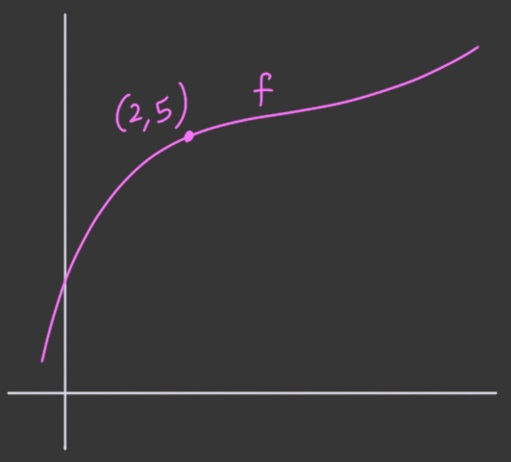
\includegraphics[scale=0.45]{img/inverse-fun.jpg}
\end{figure}

Entonces, podemos decir que $f(2) = 5$. Por consiguiente, si $f$ tiene una función inversa, esto implica que $f^{-1}(5) = 2$.

Del mismo modo, si $f(0) = 2$, entonces $f^{-1}(2) = 0$.

Ubiquemos tanto al punto $(5, \ 2)$ y $(2, \ 0)$, que pertenecen a $f^{1}$, así como a $(0, \ 2)$, que es de la función $f$, en la gráfica de arriba.

\begin{figure}[hbt!]
\centering
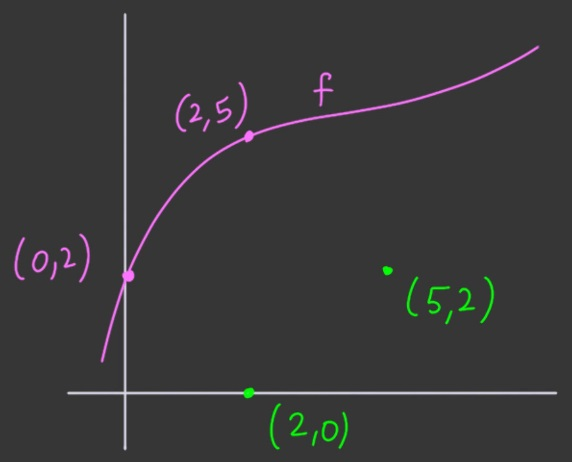
\includegraphics[scale=0.45]{img/inverse-fun-2.jpg}
\end{figure}

Como podemos apreciar, geométricamente las coordenadas de los puntos de la función $f$, se invierten en los mismos de su función inversa $f^{-1}$. O, dicho de otro modo, se intercambian los valores desde el eje X al Y, y viceversa.

En ese sentido, si trazamos una línea recta con un ángulo de $45^{o}$ con respecto al eje X (i.e., la gráfica de una función afín $y = x$), podremos ver que los valores de la función $f$ se \textbf{reflejan} en esta línea, materializándose en los valores de su función inversa $f^{-1}$.

Por lo tanto, si graficamos la curva de la función $f^{-1}$ será la misma de $f$, pero reflejada\footnote{Sigue la misma idea a como si la pusieramos frente a un espejo.} o invertida en $90^{o}$.

\newpage

\begin{figure}[hbt!]
\centering
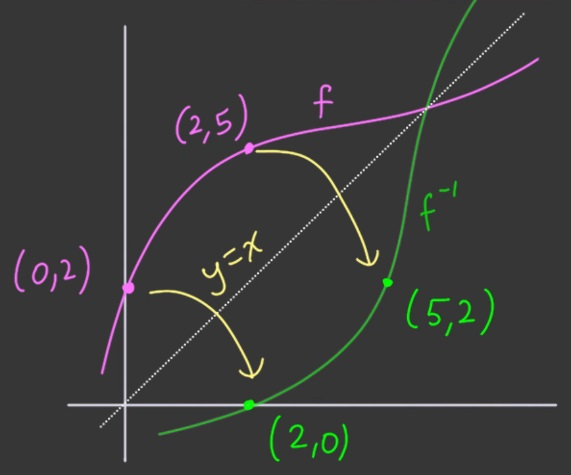
\includegraphics[scale=0.45]{img/inverse-fun-3.jpg}
\end{figure}

Ahora bien, \textbf{¿cómo comprobamos que una función tiene o no una inversa?}

Por ejemplo, tenemos una función cuadrática $f(x) = x^{2}$, de manera que tanto para $x = 2$ como para $x = -2$, $f(x) = 4$:
\[f(-2) = f(2) = 4\]
Entonces surge la pregunta sobre ¿cuál es el valor de saluda (\textit{output}) de $f^{-1}(4)$? Puede ser tanto $2$ como $-2$ y esto es un problema. Si trazamos una línea recta horizontal sobre su gráfica, podemos apreciar que corta a dos valores de $x$.

\begin{figure}[hbt!]
\centering
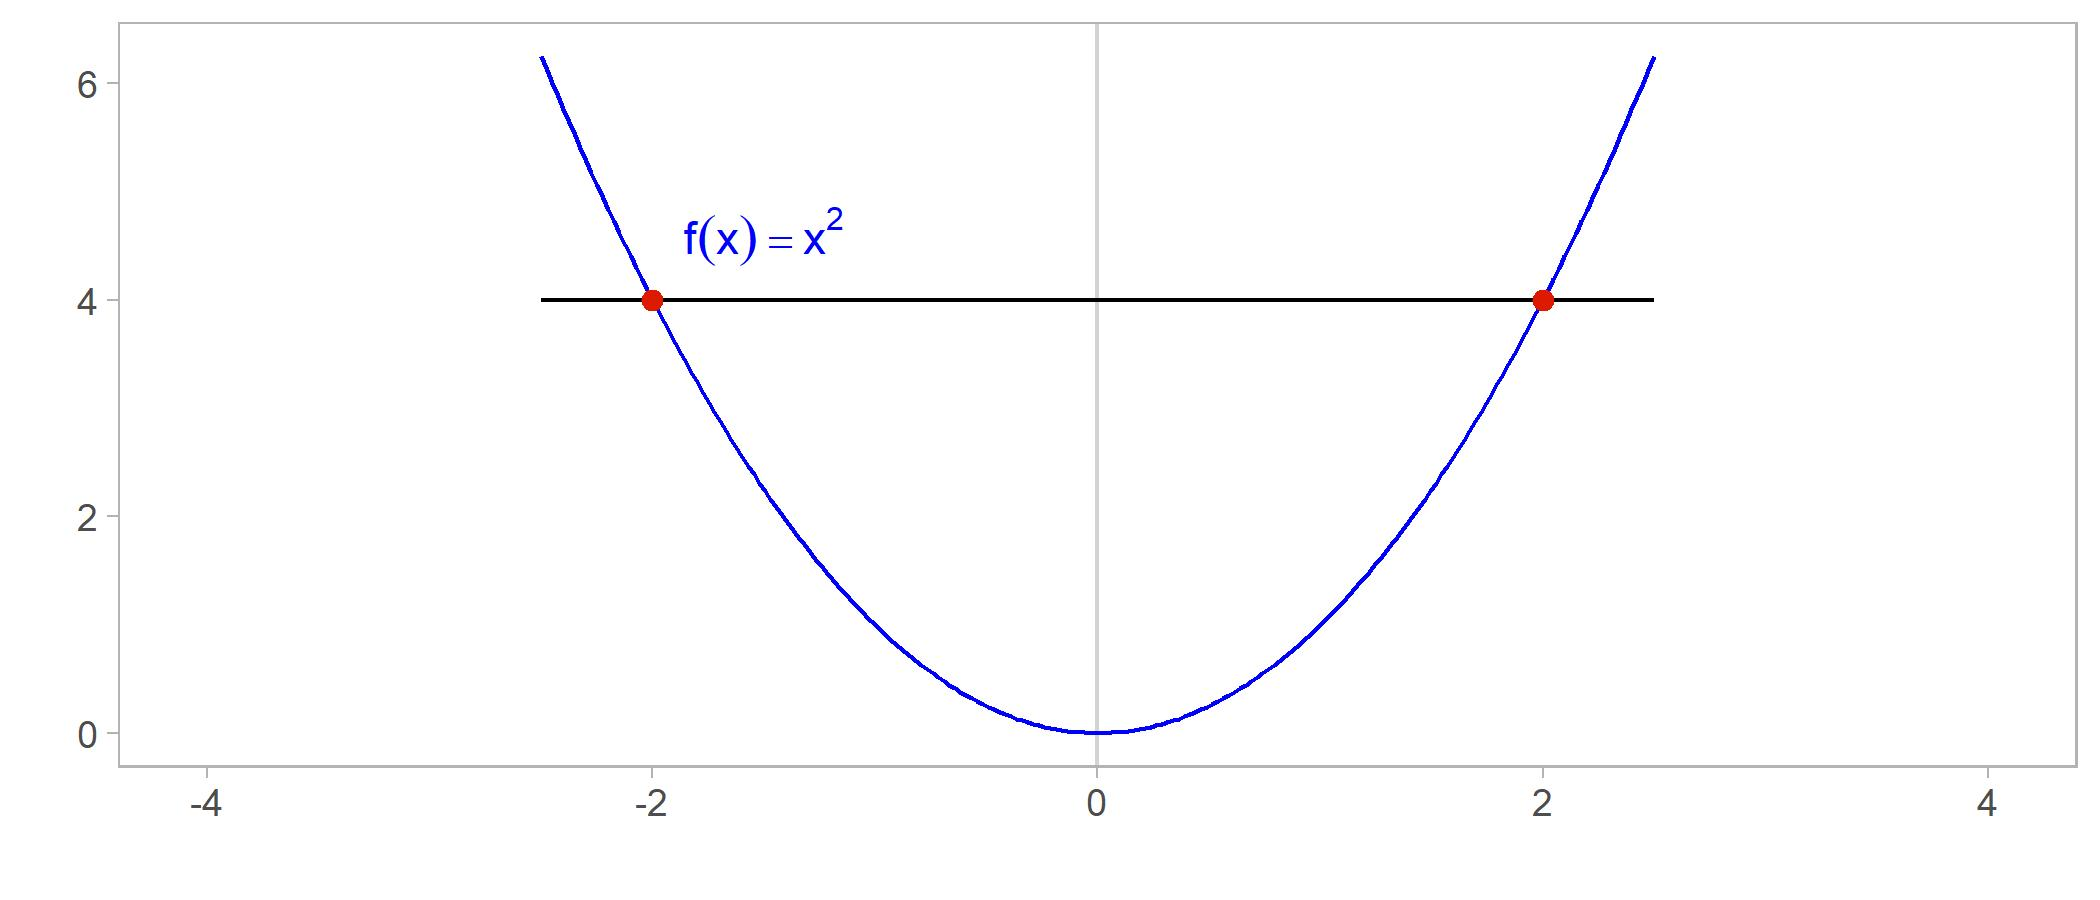
\includegraphics[scale=0.7]{img/not_one_to_one.jpg}
\end{figure}

En ese sentido, si $f(x) = x^{2}$ tuviera una función inversa $f^{-1}(x)$, entonces su gráfica (color azul) debe reflejarse en la recta de la función afín $y = x$. Esto implica, por consiguiente, que la línea recta horizontal de $f(x)$ pasará a ser la prueba de línea recta vertical en $f^{-1}(x)$ (color verde) y, como vemos en la siguiente gráfica, también se fracasa en la supuesta función inversa, por lo que $f^{-1}(x)$ tampoco no es una función.

\begin{figure}[hbt!]
\centering
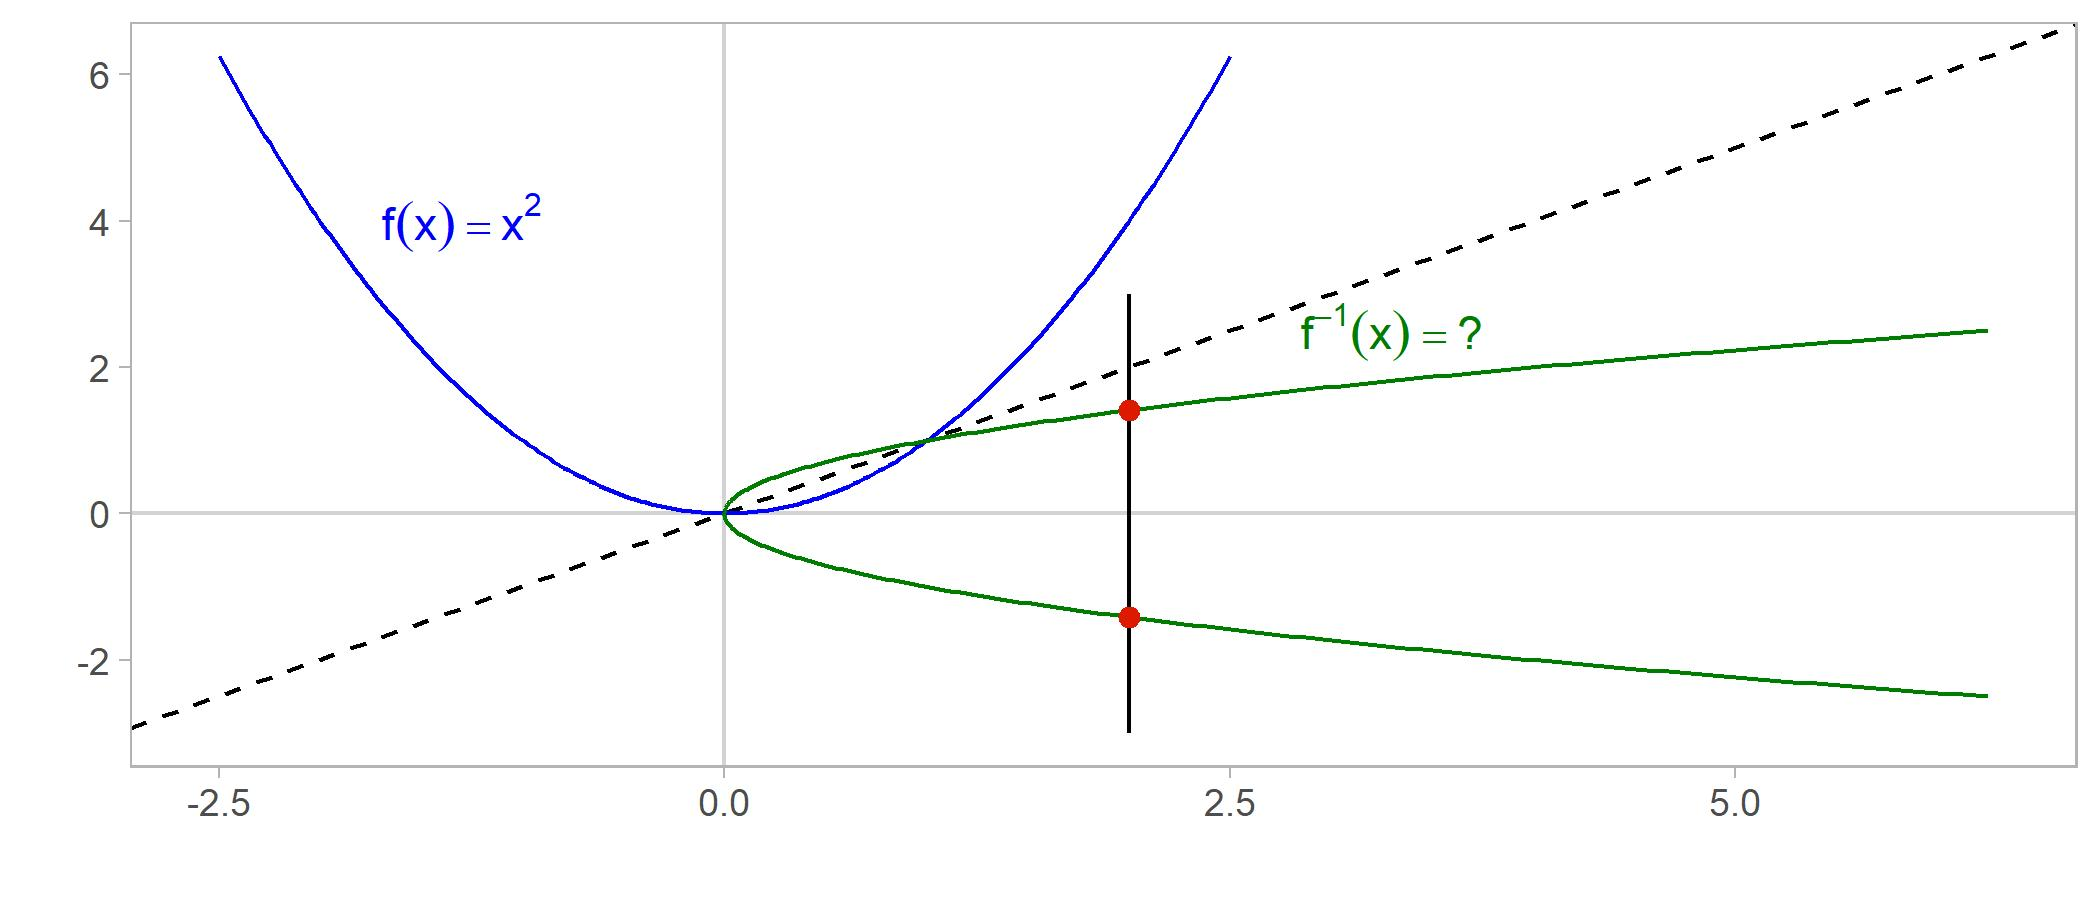
\includegraphics[scale=0.7]{img/not_one_to_one_2.jpg}
\end{figure}

Lo que podemos concluir de este caso, es que \textbf{si una función fracasa en pasar la prueba de la línea recta horizontal (si corta en más de una vez la gráfica), entonces significa que no tiene una función inversa}.

Una forma de evitar esta situación, es \textbf{dividir} (\textit{to split}) \textbf{la función} (i.e, restringir su dominio), como se ve en el siguiente gráfico.

\begin{figure}[hbt!]
\centering
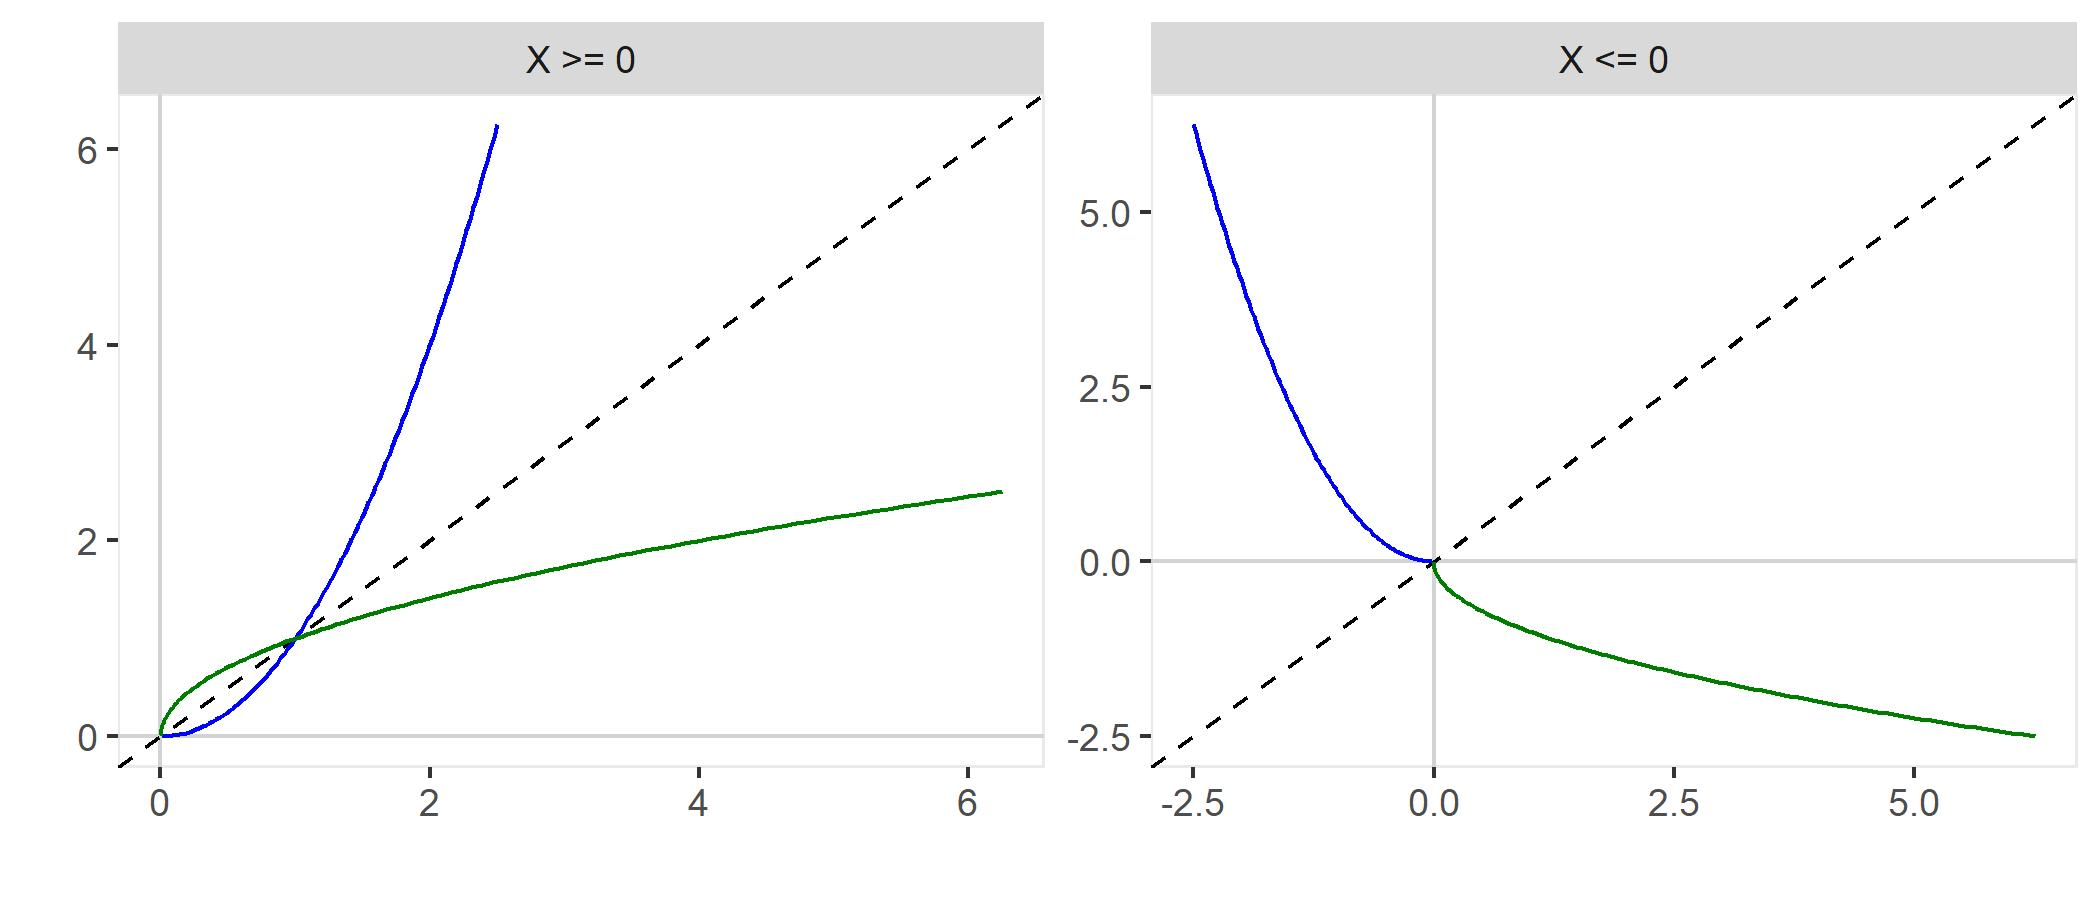
\includegraphics[scale=0.7]{img/split_not_one_to_one.jpg}
\end{figure}

En el gráfico de la izquierda (\verb|x >= 0|), tenemos la mitad derecha de la parábola $f(x) = x^{2}$ (color azul), la cual ahora sí satisface la prueba de la línea recta horizontal. Por lo tanto, tiene una función inversa y corresponde al gráfico de la \textbf{raíz cuadrada positiva} (i.e., $+\sqrt{x}$, color verde). Del mismo modo, el gráfico de la derecha (\verb|x <= 0|) se puede observar a la mitad izquierda de $f(x) = x^{2}$ (color azul) y su $f^{-1}(x)$, es la \textbf{raiz cuadrada negativa} (i.e., $-\sqrt{x}$, color verde).

Sin embargo, tanto la $+\sqrt{x}$ como la $-\sqrt{x}$ son solo \textbf{funciones inversas parciales}, ya que funcionan solo para una parte de la función original.

Veamos ahora funciones que no tienen el problema de tener el mismo \textit{output} para más de un \textit{input}. A éstas se las conoce como \textbf{funciones uno a uno} las que, al darle dos valores de entrada distintos, se obtienen dos resultados de salida únicos para cada uno. Más formalmente, se definen de la siguiente manera:

Sea $a \neq b$, entonces $f$ es una \textbf{función uno a uno} si:
\[f(a) \neq f(b)\]
En ese sentido, \textbf{si una función es ``uno a uno'', entonces tiene una función inversa}\footnote{En estricto rigor, se señala que si una función $f$ es uno a uno, con dominio $A$ y rango $B$, entonces tiene una función inversa $f^{-1}$ con dominio $B$ y rango $A$, la cual está definida por \[f^{-1}(y) = x \iff f(x) = y\] para cualquier $y$ en $B$.}.

Hay distintas formas para evaluar si una función es o no ``uno a uno''. Una de ellas, es por medio de álgebra. Específicamente, para un \textbf{output} $y$ podemos resolver la ecuación $f(x) = y$ para $x$ y demostrar, algebraicamente, que hay una sola solución para dicha igualdad.

No obstante, \textbf{una forma más fácil} de evaluar si una función es uno a uno, es \textbf{usando el Cálculo}.

Por ejemplo, tenemos la siguiente función:
\[g(x) = 2x^{3} + 3x - 1\]
Sin usar un software, podemos presumir, por ejemplo, que su gráfica puede ser como la que vemos a la izquierda en la visualización de abajo. En donde se fracasa en pasar la prueba de la línea recta horizontal. No obstante, las gráficas de las funciones cúbicas suelen ser como la que está a la derecha, donde sí se supera dicha prueba.

\begin{figure}[hbt!]
\centering
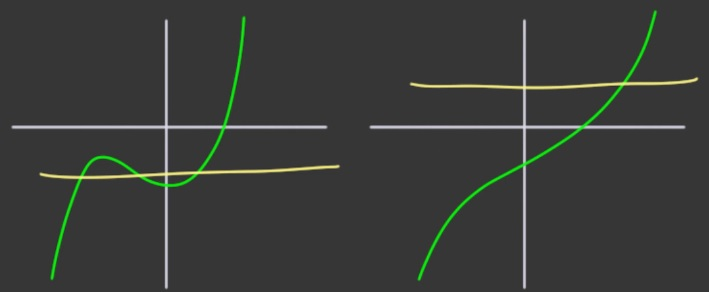
\includegraphics[scale=0.5]{img/cubic_one_to_one.jpg}
\end{figure}

Entonces, una forma para comprobar si es o no una función uno a uno, es resolverla para $x$ y ver si tiene una sola solución, pero eso sería engorroso para una función como la de $g(x)$. Otra forma más fácil para ese objetivo, es calcular su derivada.
\[\frac{d}{dx} g(x) = \frac{d}{dx}(2x^{3} + 3x - 1)\]
\[\frac{d}{dx} g(x) = 6x^{2} + 3\]
Como podemos apreciar, para cualquier valor de $x$, la $\frac{d}{dx} g(x)$ \textbf{siempre será positiva} debido a que su \textit{input} siempre se elevará al cuadrado. Esto implica que \textbf{la función $g(x)$ siempre será una función creciente}.

Por lo tanto, $g(x)$ siempre va a satisfacer la prueba de la línea recta horizontal o, en otras palabras, es una función uno a uno y, en consecuencia, tiene una función inversa.

\newpage

Volvamos al caso de las \textbf{funciones inversas parciales}. Como vimos anteriormente (pág. 67-68), para ciertos valores de $x$ la función $f(x) = x^{2}$ tiene una inversa. Es decir, \textbf{restringiendo su dominio} es posible que sea uno a uno, o que cada valor del dominio tenga una única imagen en el rango\footnote{Dominio: Conjunto de valores de entrada de una función. Rango: Conjunto de valores de salida de una función.}.

Por ejemplo, si restringimos el dominio de la función $f(x) = x^{2}$ solo a los valores mayores o iguales a cero (i.e., a $x \geq 0$), su $f^{-1}$ será la $+\sqrt{x}$. Por lo tanto, si calculamos la $\sqrt{4}$ \textbf{bajo esta condición}, entonces decimos que su resultado es el \textbf{número $x \geq 0$, cuyo cuadrado es 4}.

Entonces, las funciones inversas parciales se diferencian de las inversas completas, en que lo son bajo un dominio restringido.

Las funciones \textbf{inversas parciales}, se suelen usar en las \textbf{funciones trigonométricas}.

Por ejemplo, la función $\cos(\theta)$ claramente no es una función inversa, lo cual podemos comprobar aplicando la prueba de la recta lineal horizontal.

\begin{figure}[hbt!]
\centering
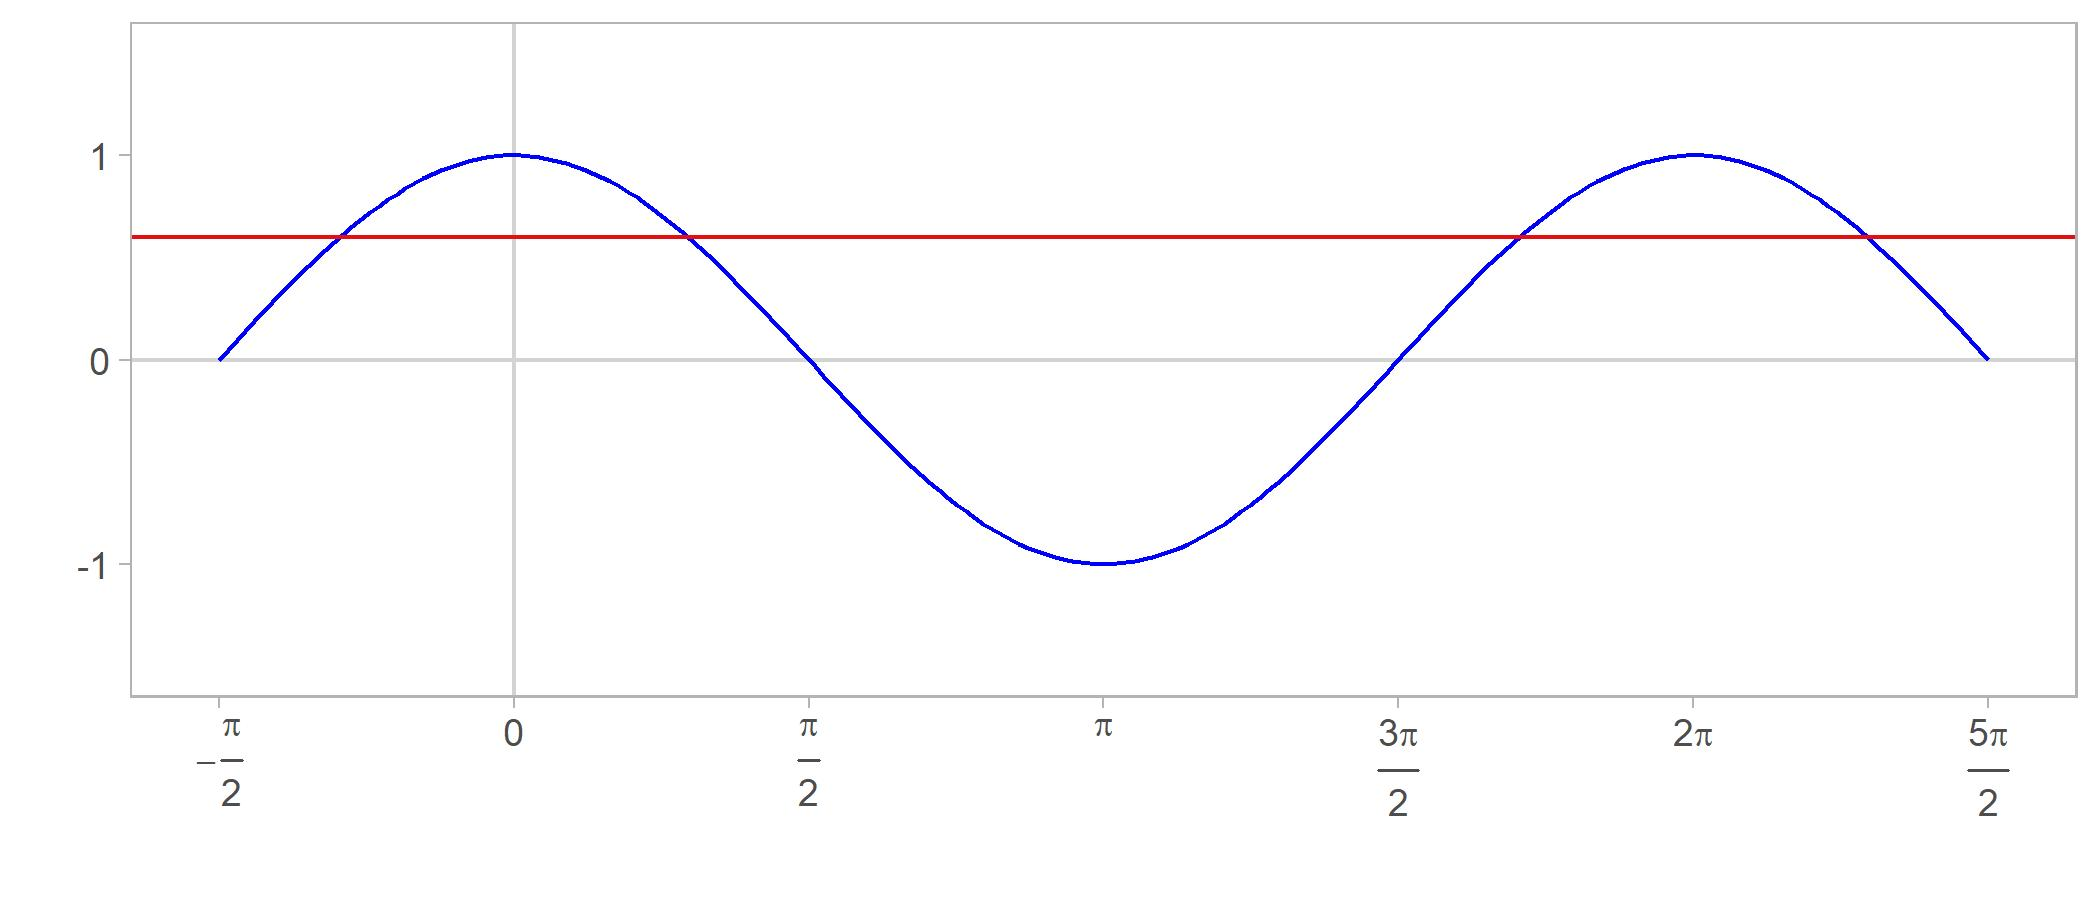
\includegraphics[scale=0.7]{img/cos_fun.jpg}
\end{figure}

Sin embargo, si restringimos su dominio en $0 \leq \theta \leq \pi$ podemos obtener su función inversa parcial. Veamos la gráfica del coseno restringido (que no es la de su inversa).

\newpage

\begin{figure}[hbt!]
\centering
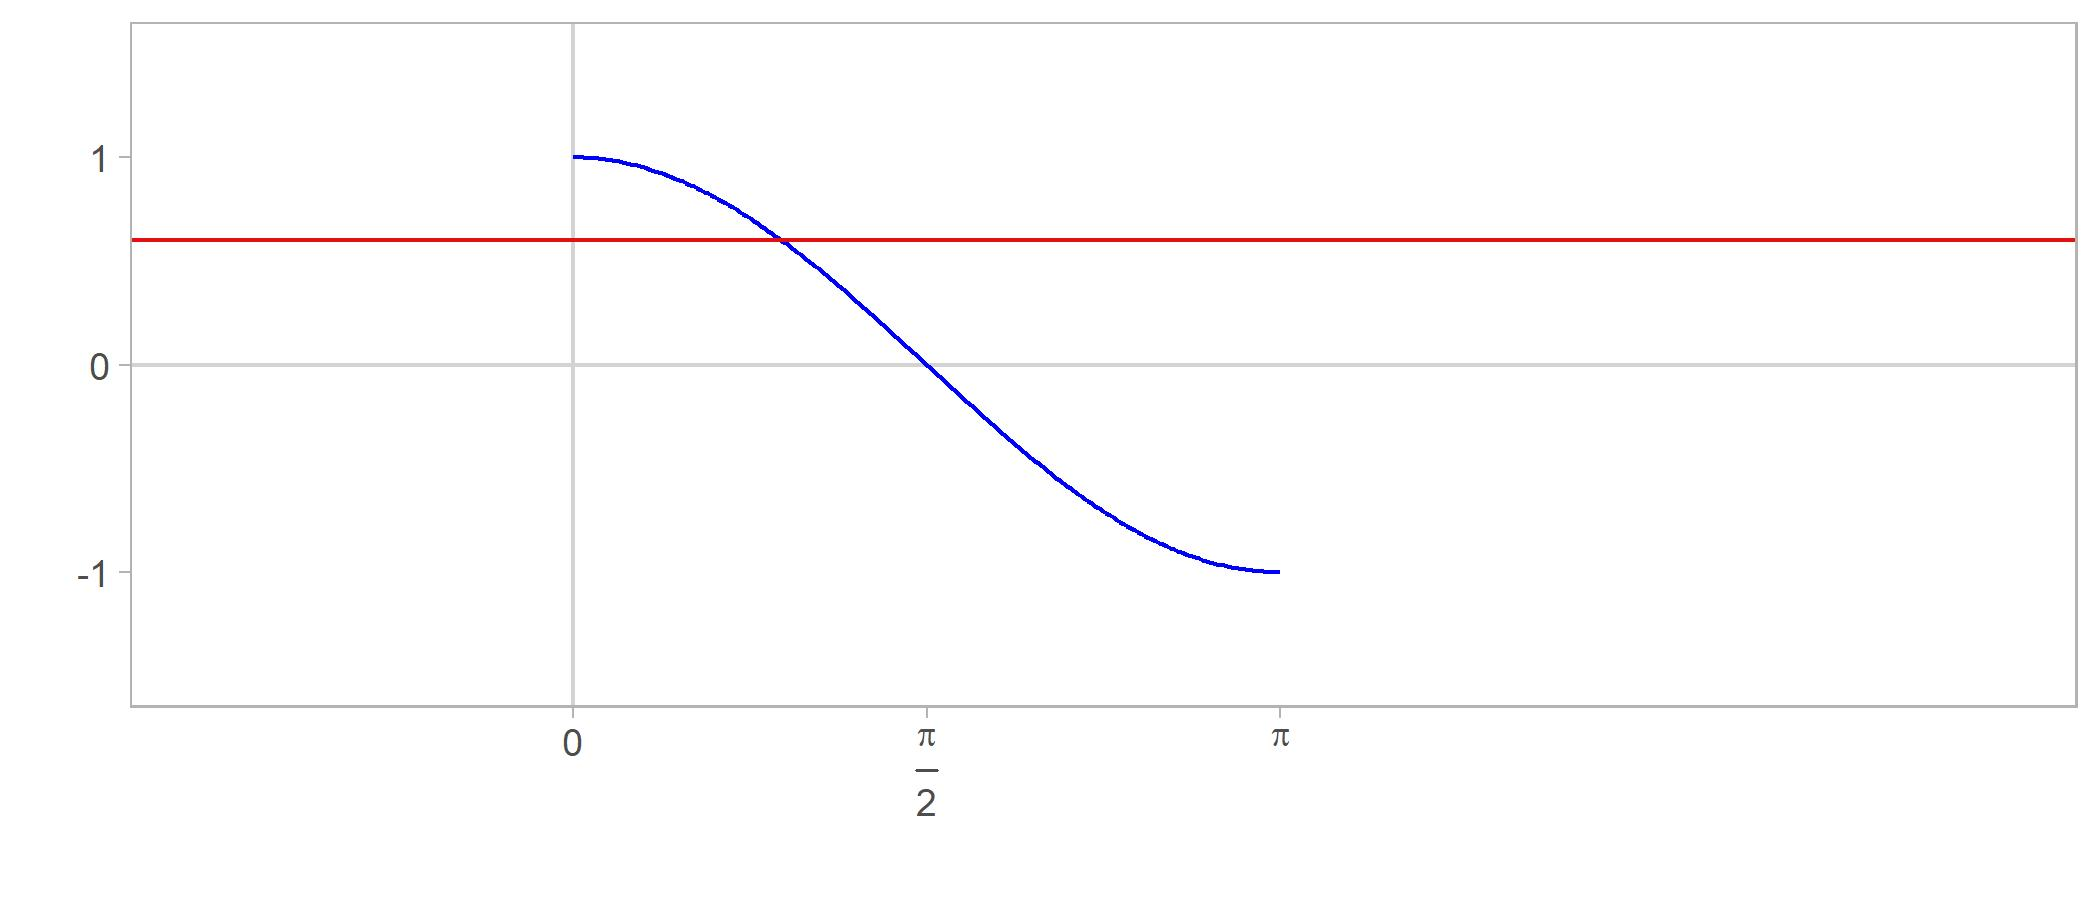
\includegraphics[scale=0.7]{img/cos_fun_restr.jpg}
\end{figure}

A la función inversa parcial del coseno se le conoce también como \textbf{arcoseno}, la cual se denota como $\arccos$ o $\cos^{-1}$. En ese sentido, el $\cos^{-1}(x)$ es \textbf{el ángulo $\theta$ en el intervalo $[0, \ \pi]$ (incluidos), tal que $\cos(\theta) = x$}.

Concentrémonos un poco en la función tangente o $\tan(x)$, cuya gráfica podemos ver a continuación.

\begin{figure}[hbt!]
\centering
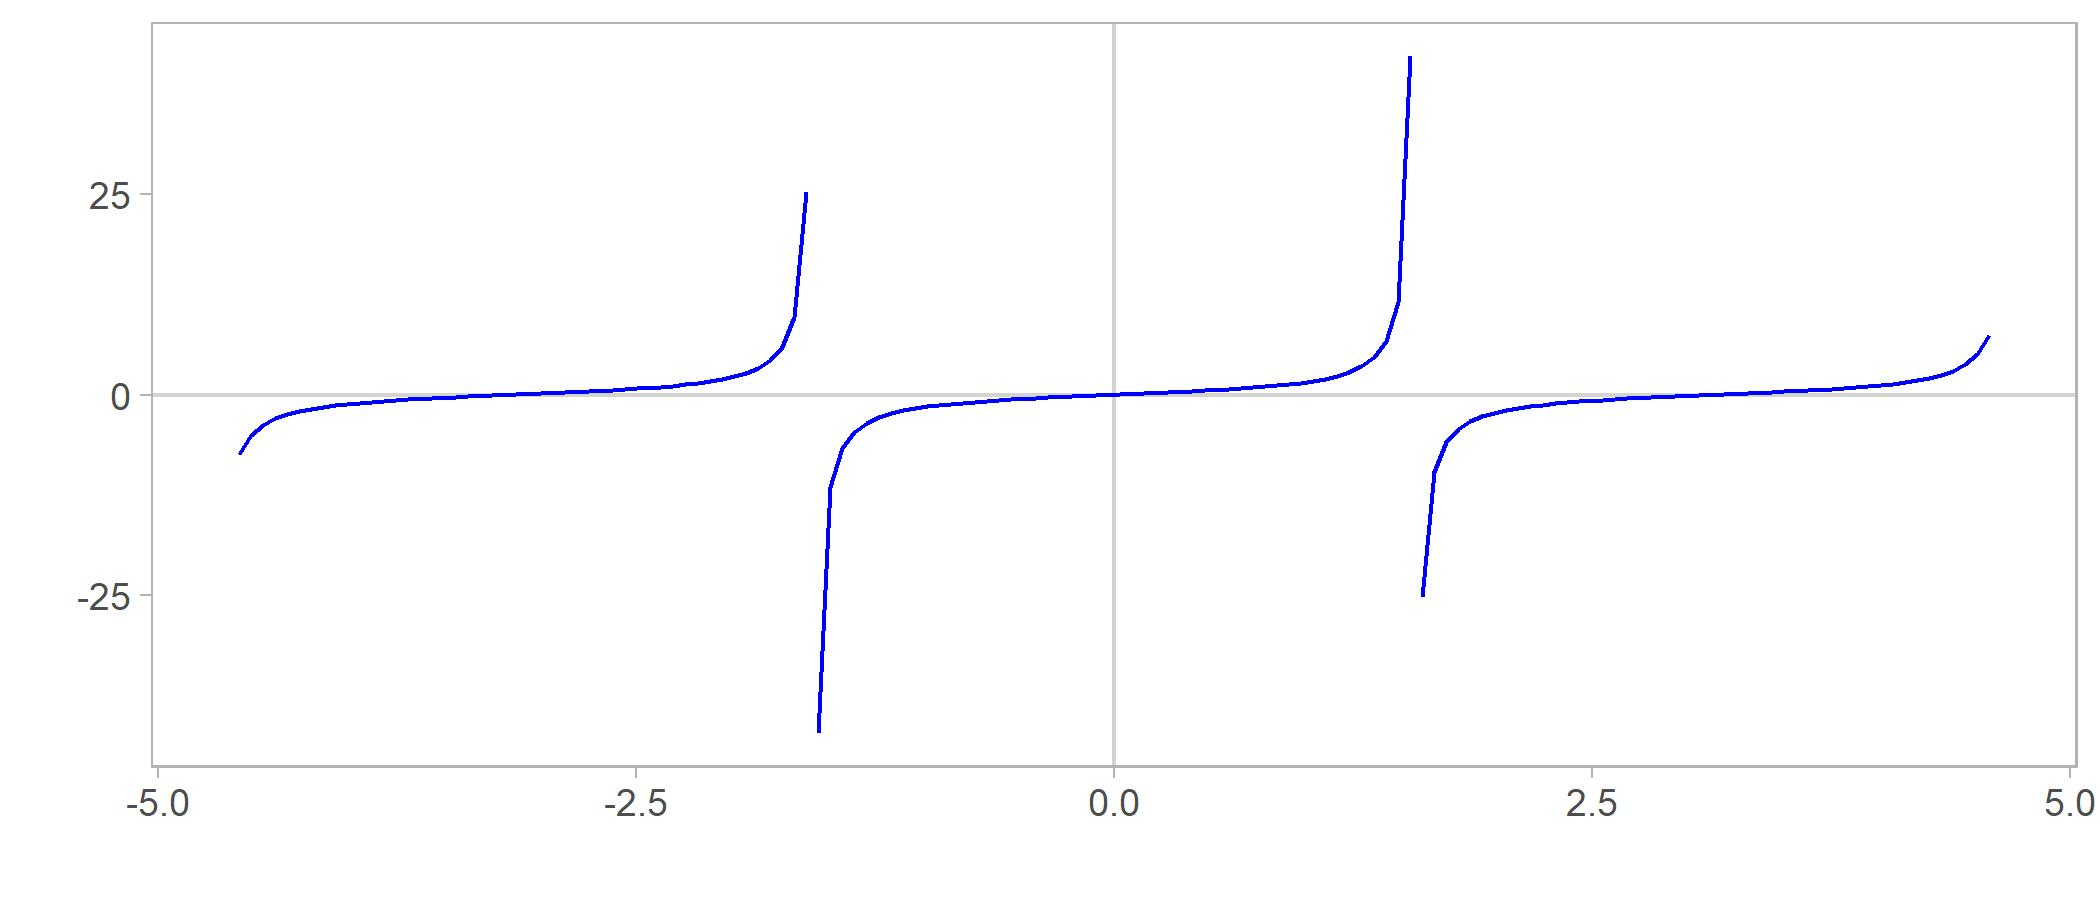
\includegraphics[scale=0.7]{img/tang_fun.jpg}
\end{figure}

Y vamos a restringir su dominio dentro del intervalo $-\frac{\pi}{2} < \theta < \frac{\pi}{2}$

\newpage

\begin{figure}[hbt!]
\centering
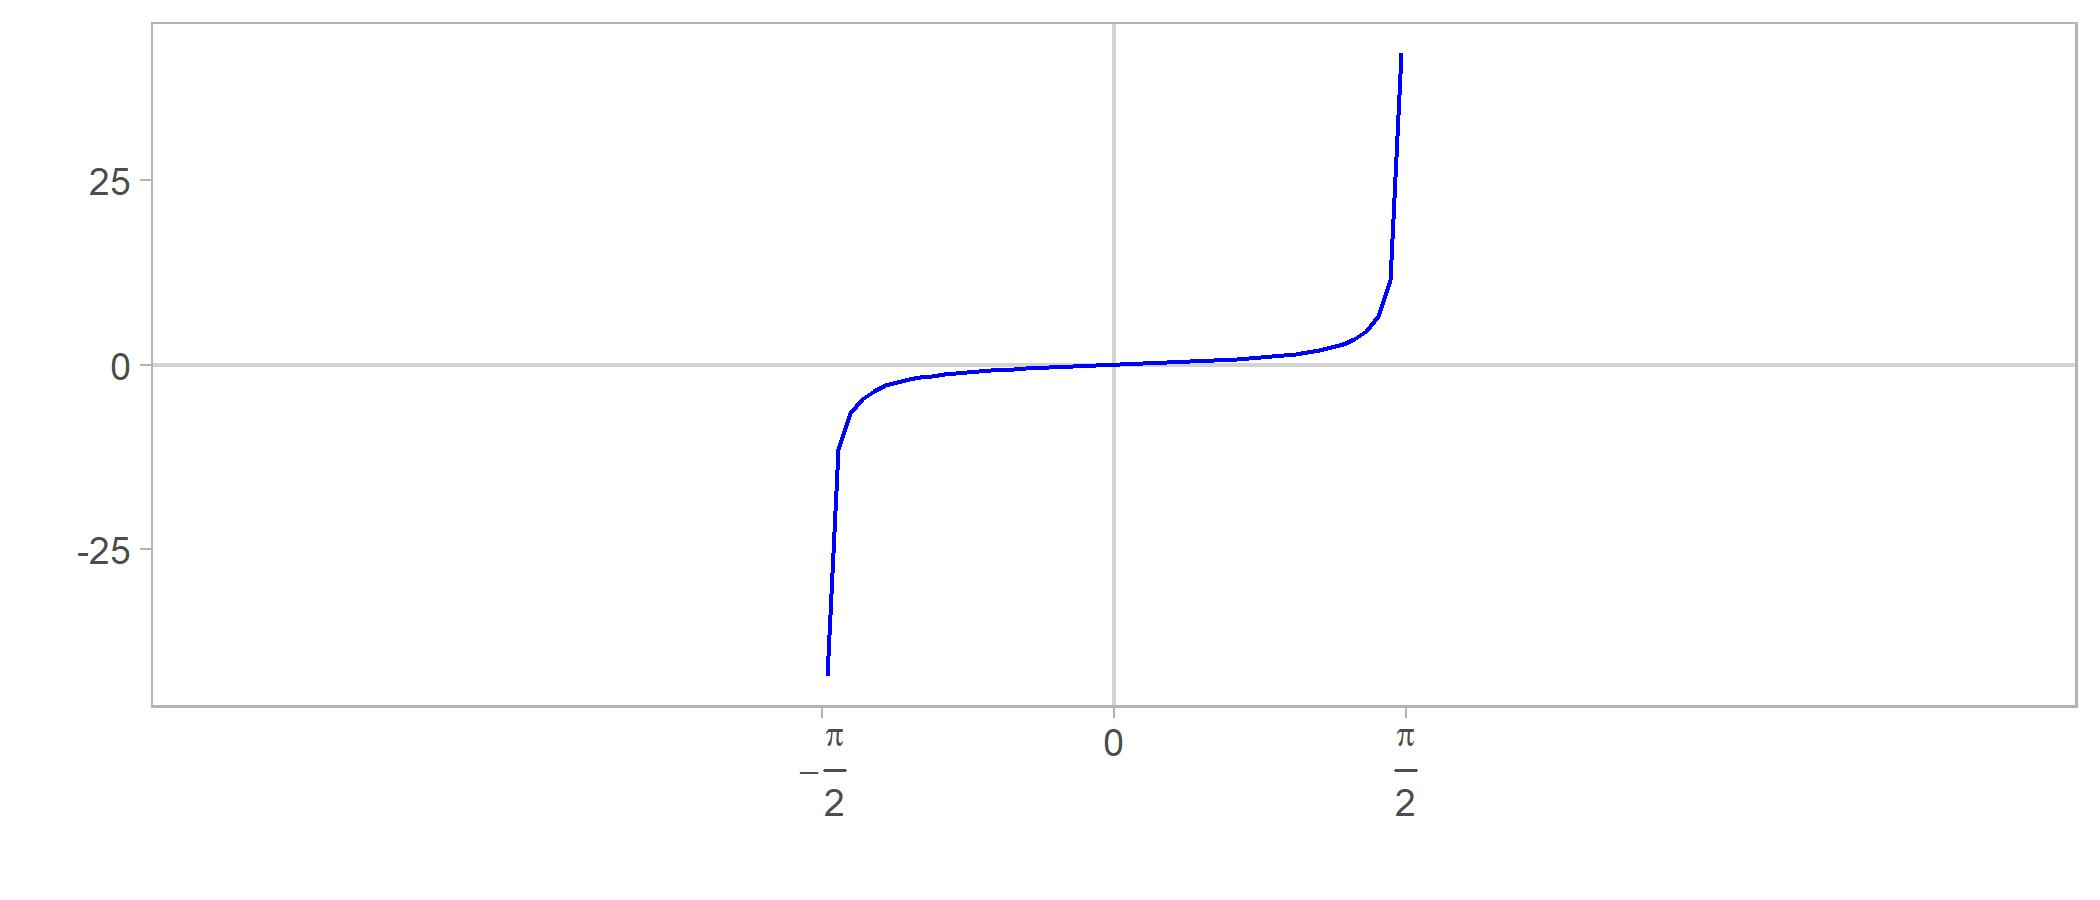
\includegraphics[scale=0.7]{img/tang_fun_restr.jpg}
\end{figure}

A diferencia del caso del $\cos(\theta)$, la desigualdad en la restricción del dominio de la $\tan(\theta)$, es estricta, ya que en $\pm\frac{\pi}{2}$, la función se indetermina.

Por consiguiente, la función inversa de la tangente, también conocida como \textbf{arcotangente}, denotada como $\arctan$ o $\tan^{-1}(x)$, será \textbf{el ángulo $\theta$ en el intervalo abierto $\left(-\frac{\pi}{2}, \ \frac{\pi}{2}\right)$, tal que $\tan(\theta) = x$}.

Entonces, en resumen con respecto algunas funciones trigonométricas y sus inversas:

\begin{itemize}
\item $\arcsin(x) = \theta$ en $\left[-\frac{\pi}{2}, \ \frac{\pi}{2}\right]$ tal que $\sin(\theta) = x$.
\item $\arccos(x) = \theta$ en $[0, \ \pi]$ tal que $\cos(\theta) = x$.
\item $\arctan(x) = \theta$ en $\left(-\frac{\pi}{2}, \ \frac{\pi}{2}\right)$ tal que $\tan(\theta) = x$.
\end{itemize}

A partir de lo anterior, podemos \textbf{combinar funciones trigonométricas con las inversas}.

Por ejemplo, el $\arccos\left(\frac{8}{9}\right)$ será un ángulo $\theta$, tal que $\cos(\theta) = \frac{8}{9}$. En ese sentido, como su resultado será un ángulo, por consiguiente, podemos calcular cualquier función trigonométrica a partir del $\arccos$.

Entonces, si el $\arccos\left(\frac{8}{9}\right) = \theta$, donde $\theta$ es un ángulo en radianes, es válido poder calcular, por ejemplo, la tangente del arcoseno:
\[\tan\left(\arccos\left(\frac{8}{9}\right)\right)\]
Si bien, hasta el momento, no sabemos el valor exacto del $\angle \theta$ (dado por el $\arccos$), sí tenemos conocimiento que se encuentra dentro del intervalo $[0, \ \pi]$ y cuyo $\cos(\theta) = \frac{8}{9}$, el cual se calcula como el cuociente entre el cateto adyacente de un triángulo rectángulo y su hipotenusa. Es decir, podemos decir que:
\[\cos(\theta) = \frac{\text{ADY}}{\text{HIP}} = \frac{8}{9}\]
Visualicemos esta información en un triángulo rectángulo.

\begin{figure}[hbt!]
\centering
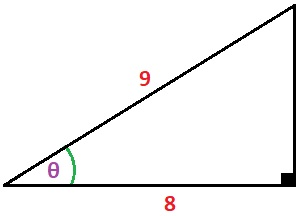
\includegraphics[scale=0.7]{img/rect-trig-inv-fun.jpg}
\end{figure}

Lo que queremos saber es la $\tan(\theta)$, que a partir de un triángulo rectángulo, se calcula como el cuociente entre el cateto opuesto y el adyacente. Ya tenemos conocimiento de la medida del adyacente que, como vemos en la imagen de arriba, es igual a $8$. Nos falta el opuesto, pero lo podemos conocer a partir del teorema de Pitágoras:
\[9 = \sqrt{8^{2} + \text{OP}^{2}}\]
\[9^{2} - 8^{2} = \text{OP}^{2}\]
\[\sqrt{17} = \text{OP}\]
Ubiquemos esta medida en el triángulo rectángulo de arriba.

\newpage

\begin{figure}[hbt!]
\centering
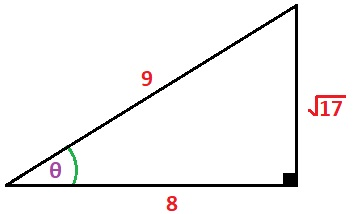
\includegraphics[scale=0.7]{img/rect-trig-inv-fun-2.jpg}
\end{figure}

Por lo tanto, sabemos que:
\[\tan(\theta) = \frac{\text{OP}}{\text{ADY}}\]
Y también sabemos que $\theta = \arccos\left(\frac{8}{9}\right)$. En consecuencia:
\[\tan\left(\arccos\left(\frac{8}{9}\right)\right) = \frac{\sqrt{17}}{8}\]




\subsection{Derivadas de Funciones Inversas.}

Veamos ahora cómo se vinculan las funciones inversas con las derivadas.

Digamos que tenemos una función $f$ y su inversa (sea completa o parcial) $f^{-1}$, que denotaremos como $g$, en la que tenemos el punto $(x, \ y)$ y es el reflejo de $(y, \ x)$ en $f$. Veamos toda esta información en la siguiente imagen.

\newpage

\begin{figure}[hbt!]
\centering
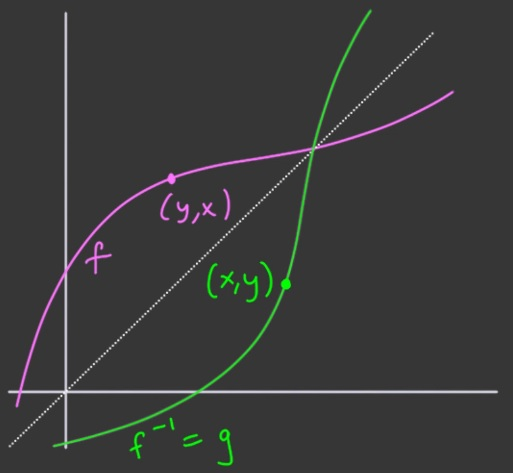
\includegraphics[scale=0.5]{img/rel-deriv-inv-fun.jpg}
\end{figure}

El vínculo que hay entre las funciones inversas y sus derivadas, es que también tienen un efecto de reflejo con respecto a las derivadas de la función original. Profundicemos en esto tanto geométricamente como usando fórmulas.

A \textbf{nivel geométrico}, lo podemos ver a partir de \textbf{las pendientes de las líneas tangentes} en los puntos $(x, \ y)$ en $g$ y $(y, \ x)$ en $f$, que corresponden a $g'(x)$ y $f'(y)$, respectivamente. Como vemos a continuación, la pendiente de $g'(x)$ es el reflejo, con respecto a la recta $y = x$, de la de $f'(y)$.

\begin{figure}[hbt!]
\centering
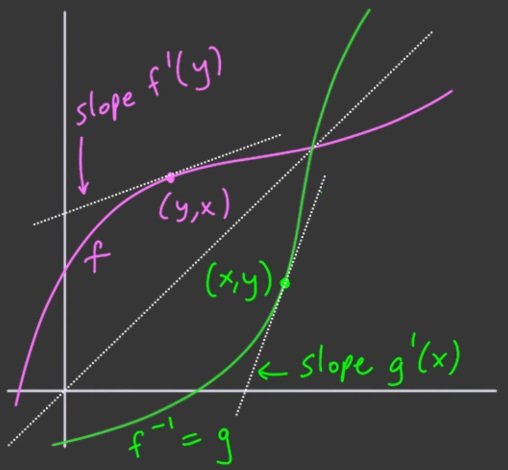
\includegraphics[scale=0.5]{img/rel-deriv-inv-fun-2.jpg}
\end{figure}

Esto también lo podemos ver en el cálculo de las pendientes de las líneas tangentes. En la derivada $f'(y)$ en $(y, \ x)$, corresponde al cuociente entre la distancia vertical y la distancia horizontal. En $g'(x)$ del punto $(x, \ y)$, dichas distancias se ``invierten''. Es decir, la distancia vertical de $f'(y)$ corresponde a la distancia horizontal en $g'(x)$, mientras que la distancia horizontal en $f'(y)$ pasa a ser la distancia vertical en $g'(x)$.

\begin{figure}[hbt!]
\centering
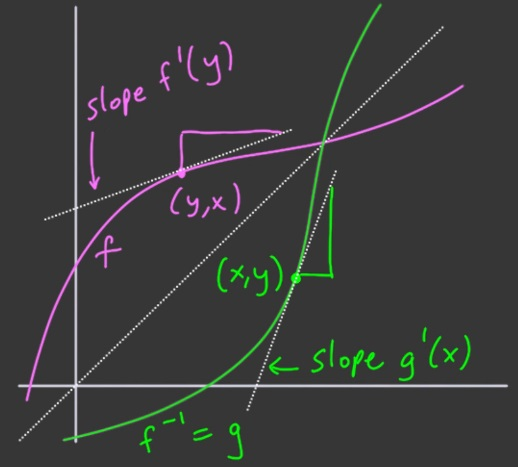
\includegraphics[scale=0.5]{img/rel-deriv-inv-fun-3.jpg}
\end{figure}

En otras palabras, podemos decir que $f'(y)$ y $g'(x)$, son \textbf{recíprocas}\footnote{También conocido como \textbf{inverso multiplicativo}. Por ejemplo, el inverso multiplicativo de un valor $x$ es $x^{-1} = \frac{1}{x}$. Otro ejemplo, es el de la función $\sin(x)$, que corresponde a la $\text{cosec}(x)$. La denotación es similar a la de las funciones inversas, pero no son lo mismo, así que ¡ha evitar confundiarlas!}.

Por ejemplo, podemos decir que la distancia vertical de $g'(x)$ en $(x, \ y)$, es $5$, mientras que la distancia horizontal en el mismo punto, es $2$. Por lo tanto, $g'(x) = \frac{5}{2}$. Y, al ser recíproca de $f'(y)$, entonces $f'(y) = \frac{2}{5}$.

\newpage

\begin{figure}[hbt!]
\centering
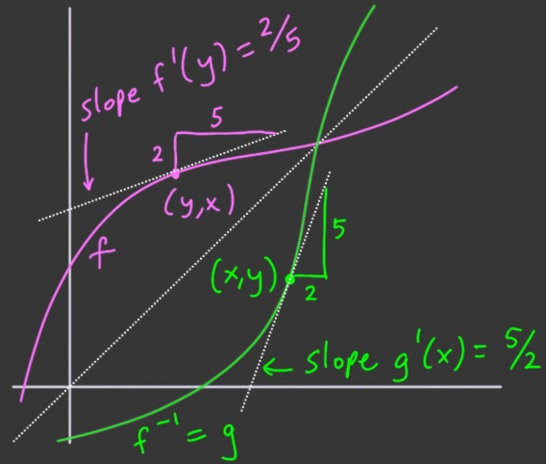
\includegraphics[scale=0.5]{img/rel-deriv-inv-fun-4.jpg}
\end{figure}

Por lo tanto, lo que hemos estado señalando es que, si $g = f^{-1}$, entonces:
\[g'(x) = \frac{1}{f'(y)} = \frac{1}{f'(g(x))}\]
Y la derivada de esta función inversa puede aplicarse siempre y cuando $f$ tenga una línea tangente reflejándose. Es decir, mientras $f'(g(x))$ exista y sea distinto de cero. Si es igual a cero, entonces la gráfica de $f'(g(x))$ será una línea horizontal (i.e., sin pendiente) y, su reflejo en $g'(x)$, será por consiguiente, una línea vertical o, en otras palabras, su pendiente estará indefinida.

Lo anterior también puede ser visto usando \textbf{fórmulas}. Por ejemplo, digamos que:
\[f(g(x)) = x \quad \text{para todos los }x\]
A partir de la definición de las funciones inversas, la expresión de arriba es verdadera. En ese sentido, podemos derivar ambos lados de la ecuación (asumiendo que tanto $f(y)$ como $g(x)$, son derivables), con respecto a $x$.
\[\frac{d}{dx}f(g(x)) = \frac{d}{dx} x\]
Como vemos, en el lado izquierdo podemos aplicar la regla de la cadena, al ser una función compuesta. Mientras que el lado derecho es igual a $1$.
\[\frac{d}{d \ g(x)}f(g(x)) \cdot \frac{d}{dx} g(x) = 1\]
Usando la notación de Newton, esto es lo mismo que:
\[f'(g(x)) \cdot g'(x) = 1\]
Despejemos $g'(x)$, que es lo que nos importa:
\[g'(x) = \frac{1}{f'(g(x))}\]
Así hemos conseguido la \textbf{fórmula para derivar funciones inversas}, la cual podemos usar tanto en funciones inversas completas (i.e., que provienen de una función uno a uno), como en funciones inversas parciales.

Veamos un ejemplo.

Sea la función $f(x) = -2x^{3} - 7x + 5$ del tipo ``uno a uno'' y que, por tanto, tiene una función inversa. Si $g = f^{-1}$, busque $g(5)$ y $g'(5)$.

Como $g$ es la función inversa de $f(x)$, entonces podemos decir que:
\[g(5) = x \iff f(x) = 5\]
Podemos aprovechar la igualdad de $f(x)$ para buscar el valor de $x$ en $f(x) = 5$.
\[5 = f(x)\]
\[5 = -2x^{3} - 7x + 5\]
Observemos bien la igualdad de arriba y contestemos la siguiente pregunta: ¿A qué valor de $x$ la parte de la izquierda de la ecuación se iguala a $5$?

Si simplemente decimos que $x = 0$, entonces la igualdad se cumple:
\[5 = -2(0^{3}) - 7(0) + 5\]
\[5 = 5\]
Entonces, podemos volver a la relación inicial para decir lo siguiente:
\[g(5) = 0 \iff f(0) = 5\]
Lo cual es verdadero. Es decir, $g(5) = 0$, que es la primera respuesta que nos piden.

Luego, nos piden calcular la derivada de la función inversa $g$ en $x = 5$. Como sabemos, su fórmula es la recíproca de la derivada de la función original. Es decir:
\[g'(x) = \frac{1}{f'(g(x))}\]
Primero, calculemos la derivada de $f'(x)$.
\[f'(x) = -2x^{3} - 7x + 5\]
\[f'(x) = -6x^{2} - 7\]
Por lo tanto:
\[g'(x) = \frac{1}{-6 \cdot (g(x))^{2} - 7}\]
Lo que buscamos es $g'(5)$ y sabemos que $g(5) = 0$. Por consiguiente:
\[g'(5) = \frac{1}{-6 \cdot (g(5))^{2} - 7} = \frac{1}{-6 \cdot (0)^{2} - 7} = - \frac{1}{7}\]
Volvamos a concentrarnos en las funciones trigonométricas. En particular, \textbf{usemos la fórmula para derivar funciones inversas para calcular la derivada del $\arcsin$}.

Si aplicamos la fórmula, podemos expresarla de la siguiente manera:
\[\frac{d}{dx} \arcsin(x) = \frac{1}{\sin'(\arcsin(x))}\]
Sabemos que $\sin'(\theta) = \cos(\theta)$, por lo tanto:
\[\frac{d}{dx} \arcsin(x) = \frac{1}{\cos(\arcsin(x))}\]
También sabemos que el $\arcsin(x)$ es la función inversa parcial del $\sin(\theta)$, en donde:
\[\arcsin(x) = \theta \ \text{en } x = \left[- \frac{\pi}{2}, \ \frac{\pi}{2}\right] \iff \sin(\theta) = x\]

Entonces, cumpliendo la condición de arriba con respecto al $\arcsin(x)$, podemos decir que:
\[\frac{d}{dx} \arcsin(x) = \frac{1}{\cos(\arcsin(x))} = \frac{1}{\cos(\theta)}\]
Si volvemos a la condición para que $\arcsin(x) = \theta$, entonces podemos decir que:
\[\sin(\theta) = \frac{x}{1}\]
Y sabemos que $\sin(\theta) = \frac{\text{OP}}{\text{HIP}}$. Entonces:
\[\sin(\theta) = \frac{\text{OP}}{\text{HIP}} = \frac{x}{1}\]
Esta información la podemos llevar a un triángulo rectángulo.

\begin{figure}[hbt!]
\centering
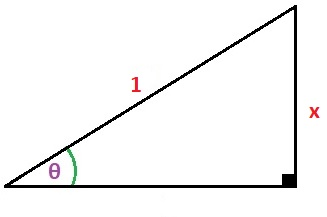
\includegraphics[scale=0.7]{img/rect-trig-deriv-arcsin.jpg}
\end{figure}

Ahora bien, lo que necesitamos saber para calcular la $\frac{d}{dx} \arcsin(x)$, es el $\cos(\theta)$ y para obtenerlo, necesitamos el cateto adyacente a $\theta$ del triángulo rectángulo de arriba. Dicho cateto lo podemos encontrar usando el teorema de Pitágoras:
\[1 = \sqrt{x^{2} + (\text{ADY})^{2}}\]
\[1 - x^{2} = (\text{ADY})^{2}\]
\[\sqrt{1 - x^{2}} = \text{ADY}\]

Agreguemos esta nueva información al triángulo rectángulo de arriba.

\newpage

\begin{figure}[hbt!]
\centering
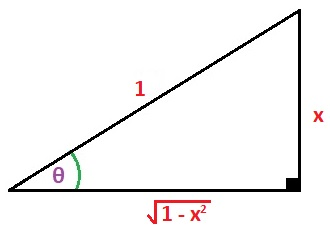
\includegraphics[scale=0.7]{img/rect-trig-deriv-arcsin-2.jpg}
\end{figure}

Entonces, con esta información, podemos calcular el $\cos(\theta)$:
\[\cos(\theta) = \frac{\text{ADY}}{\text{HIP}} = \frac{\sqrt{1 - x^{2}}}{1} = \sqrt{1 - x^{2}}\]
Y podemos llevar esta información a la $\frac{d}{dx} \arcsin(x)$, para conocer su fórmula:
\[\frac{d}{dx} \arcsin(x) = \frac{1}{\cos(\theta)} = \frac{1}{\sqrt{1 - x^{2}}}\]
Si $x < 0$, podemos deducir a partir de la circunferencia unitaria, que $\theta$ será un valor negativo, pero dentro del intervalo $\left(- \frac{\pi}{2}, \ 0\right)$. No obstante, como podemos ver a continuación, por la ubicación del $\cos(\theta) = \sqrt{1 - x^{2}}$ en el cuadrante, siempre será positivo.

\begin{figure}[hbt!]
\centering
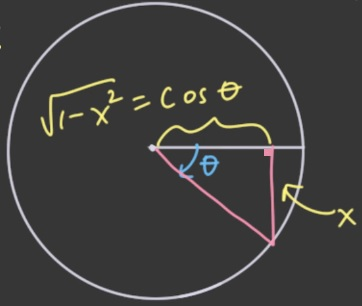
\includegraphics[scale=0.6]{img/deriv-arcsin-unit-circ.jpg}
\end{figure}

Sin embargo, si volvemos a la fórmula de la $\frac{d}{dx} \arcsin(x)$, $x$ debe restringirse al intervalo abierto $(-1, \ 1)$, ya que para dichos valores, la derivada se indetermina. Aunque el dominio del $\arcsin(x)$ corresponde al intervalo cerrado $[-1, \ 1]$, por lo que en dichos puntos, las líneas tangentes serán líneas verticales, como lo podemos ver en la siguiente gráfica (líneas verdes).

\newpage

\begin{figure}[hbt!]
\centering
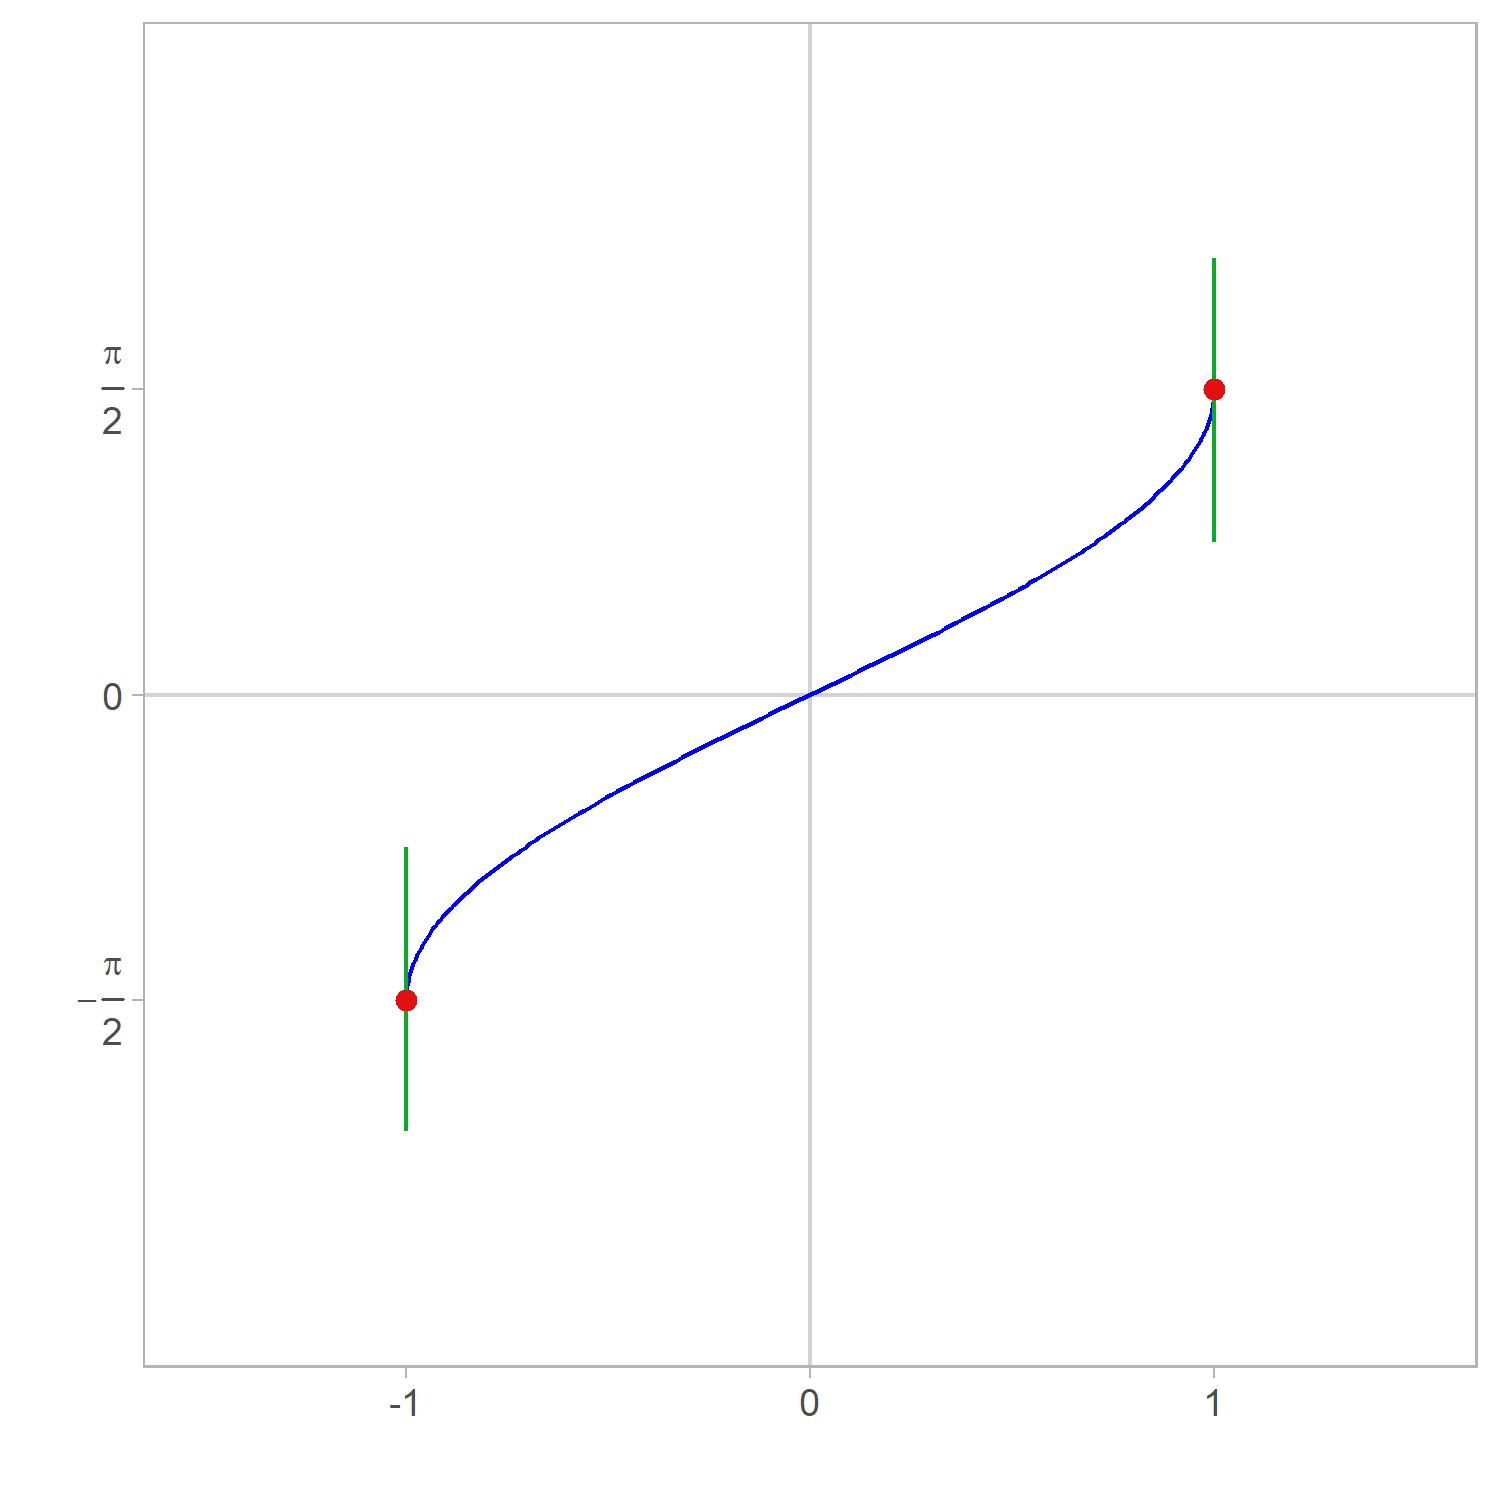
\includegraphics[scale=0.6]{img/tan_lines_arcsin.jpg}
\end{figure}

Del mismo modo, podemos buscar las fórmulas de las derivadas de las funciones inversas parciales del coseno y la tangente de un ángulo, cuyas fórmulas resumimos a continuación (junto con la del $\arcsin(x)$):
\[
\frac{d}{dx} \arccos(x) = - \frac{1}{\sqrt{1 - x^{2}}}; \quad \frac{d}{dx} \arctan(x) = \frac{1}{1 + x^{2}}; \quad \frac{d}{dx} \arcsin(x) = \frac{1}{\sqrt{1 - x^{2}}}
\]

\newpage



\subsection{Funciones Exponenciales.}

Las funciones exponenciales son aquellas en donde, el valor que varía, se encuentra en el exponente. Veamos un ejemplo de ellas:
\[f(x) = 2^{x}\]
Grafiquemos algunos puntos a partir de $f(x)$, así como su curva.
Los puntos estarán dados por los pares ordenados que se ven en la siguiente tabla:

\begin{table}[hbt!]
\centering

\begin{tabular}{c | c c c c c}
$x$ & $-2$ & $-1$ & $0$ & $1$ & $2$ \\
\hline
$f(x)$ & $0.25$ & $0.5$ & $1$ & $2$ & $4$
\end{tabular}

\end{table}


\begin{figure}[hbt!]
\centering
\includegraphics[scale=0.7]{img/exp_plot.jpg}
\end{figure}

En primer lugar, podemos observar que la curva a todos los valores reales de $x$, tanto positivos como negativos. Es decir, su dominio está definido para todos los $\mathbb{R}$.

Por otra parte, a cada valor entero de $x$, la función $f(x)$ se va agrandando o achicando muy rápidamente. En este caso, va aumentando el doble cuando nos movemos en valores de $x > 0$; y va disminuyendo por la mitad para valores de $x < 0$, acercándose a cero en pocos valores. No obstante, para cualquier valor de $x$, $f(x)$ \textbf{siempre será positiva}.

Podemos generalizar una función exponencial del siguiente modo:
\[f(x) = a^{x}\]
Donde siempre será \textbf{continua} para $a > 1$. Si $a \leq 0$, la función se indetermina; y si $a = 1$, se convierte en una función constante.

Si cambiamos la base (i.e., $a$), ésta alterará la \textbf{forma} de la curva de la función exponencial.

Por ejemplo, en el siguiente gráfico tenemos tres funciones exponenciales, cuyas bases son $2$, $3$ y $5$. Como vemos, mientras más grande es la base, más empinada (curvada hacia la izquierda) es su gráfica.

\begin{figure}[hbt!]
\centering
\includegraphics[scale=0.7]{img/exp_plot_2.jpg}
\end{figure}

No obstante, el comportamiento de las tres funciones exponenciales siguen siendo las mismas.

Antes de avanzar, no olvidemos las propiedades de los exponentes:

Sea $a$ un número real positivo.

\begin{itemize}
\item $a^{0} = 1$
\item $a^{1} = a$
\item $a^{m} \cdot a^{n} = a^{m + n}$
\item $(a^{m})^{n} = a^{m \cdot n}$
\item $a^{m/n} = \sqrt[n]{a^{m}}$
\end{itemize}

Ahora vayamos a derivar la función exponencial $a^{x}$ y, para comenzar, respondamos la siguiente pregunta: ¿por qué \underline{\textbf{no}} podemos usar la regla de la potencia para derivar $a^{x}$?

Recordemos que la fórmula de la regla de la potencia es $\frac{d}{dx} x^{n} = n \cdot x^{n - 1}$, en donde el exponente $n$ es un número fijo, mientras que la base $x$ varía. Anteriormente (pág. 83) dijimos que en las funciones exponenciales, cuya forma es $a^{x}$ ,el exponente $x$ es el que varía y la base $a$ se mantiene fija, por lo que aplicar esta regla no es factible para este caso. Así que la descartamos.

Otro método que podemos usar para buscar la derivada de $a^{x}$, es la definición de la derivada. Es decir, el cálculo de la pendiente de la línea tangente.
\[\frac{d}{dx} f(x) = \lim_{\Delta x \to 0} \frac{f(x + \Delta x) - f(x)}{\Delta x}\]
Para el caso de $a^{x}$, la denotamos como sigue:
\[\frac{d}{dx} a^{x} = \lim_{\Delta x \to 0} \frac{a^{x + \Delta x} - a^{x}}{\Delta x}\]
Si observamos el numerador de la fracción, $a^{x + \Delta x} = a^{x} \cdot a^{\Delta x}$. Es decir:
\[\frac{d}{dx} a^{x} = \lim_{\Delta x \to 0} \frac{a^{x} \cdot a^{\Delta x} - a^{x}}{\Delta x}\]
Lo que nos lleva a tener a $a^{x}$ como el término común en el numerador, así que podemos factorizarlo y tener la siguiente expresión.
\[\frac{d}{dx} a^{x} = \lim_{\Delta x \to 0} a^{x} \cdot \left(\frac{a^{\Delta x} - 1}{\Delta x}\right)\]
Algo interesante de esta expresión, es que en el cálculo del límite, lo que está variando es $\Delta x$, ya que se está moviendo a cero desde la izquierda y la derecha. Esto nos lleva a asumir que $a^{x}$ está fijo o se mantiene \textbf{constante}. Por lo tanto, podemos aplicar la regla del límite del múltiplo constante:
\[\lim_{x \to a}[c \cdot f(x)] = c \cdot \lim_{x \to a} f(x)\] 
Aplicándolo al cálculo de la derivada de $a^{x}$:
\[\frac{d}{dx} a^{x} = a^{x} \cdot \lim_{\Delta x \to 0} \left(\frac{a^{\Delta x} - 1}{\Delta x}\right)\]

Entonces, hasta ahora sabemos que la $\frac{d}{dx} a^{x}$ es el producto entre $a^{x}$ y un número que desconocemos. A este ``número misterioso'' lo definiremos como $M(a)$. Es decir:
\[M(a) = \lim_{\Delta x \to 0} \left(\frac{a^{\Delta x} - 1}{\Delta x}\right)\]
Por lo tanto:
\[\frac{d}{dx} a^{x} = a^{x} \cdot M(a)\]
Ahora, veamos qué ocurre cuando definimos la derivada en $x = 0$.
\[\left.\frac{d}{dx} a^{x}\right|_{x = 0} = a^{0} \cdot M(a)\]
\[\left.\frac{d}{dx} a^{x}\right|_{x = 0} =  M(a)\]
En otras palabras, podemos decir que \textbf{$M(a)$ es la pendiente del gráfico de $a^{x}$ en $x = 0$}.

Entonces, si volvemos al gráfico de $f(x) = 2^{x}$ y trazamos la linea tangente en $x = 0$, su pendiente será $m = M(2)$.

\begin{figure}[hbt!]
\centering
\includegraphics[scale=0.7]{img/exp_plot_3.jpg}
\end{figure}

Por lo tanto, para conocer el valor de la derivada en toda la curva de $2^{x}$, necesitamos ser capaces de saber el valor específico de $M(2)$.

Una forma de acercarnos al valor de $M(2)$, es usando la definición de $M(a)$:
\[M(2) = \lim_{\Delta x \to 0} \left(\frac{2^{\Delta x} - 1}{\Delta x}\right)\]
Es decir, ver a qué valor se aproxima $M(2)$ a medida que $\Delta x \to 0$. Veámoslo en la siguiente tabla:

\begin{table}[hbt!]
\centering

\begin{tabular}{c | c c c c c c}
$\Delta x$ & $-0.1$ & $-0.01$ & $-0.001$ & $0.001$ & $0.01$ & $0.1$\\
\hline
$M(2)$ & $0.669$ & $0.690$ & $0.692$ & $0.693$ & $0.695$ & $0.717$
\end{tabular}

\end{table}

Como vemos, a medida que $\Delta x \to 0$, $M(2) \to \approx 0.69$. En otras palabras, lo que estamos diciendo es que la derivada en $x = 0$ de $2^{x}$ es aproximado a ese valor:
\[\left. \frac{d}{dx} 2^{x} \right |_{x = 0} = M(2) \approx 0.69\]
Si aumentamos la base, ¿qué debería ocurrir con la derivada del exponencial en $x = 0$?

Por ejemplo, digamos que la base $a = 4$. Anteriormente (pág. 84) señalamos que, a medida que aumenta la base de un número exponencial, su gráfica se hace más empinada. Por lo tanto, a partir de esta información podemos presumir que la pendiente de la línea tangente en $x = 0$ de $4^{x}$ es mayor a la de $2^{x}$ en el mismo punto.

Veamos el cálculo de $M(4)$, cuya fórmula es:
\[M(4) = \lim_{\Delta x \to 0} \left(\frac{4^{\Delta x} - 1}{\Delta x}\right)\]
Y los resultados los vemos en la tabla de a continuación.

\newpage

\begin{table}[hbt!]
\centering

\begin{tabular}{c | c c c c c c}
$\Delta x$ & $-0.1$ & $-0.01$ & $-0.001$ & $0.001$ & $0.01$ & $0.1$\\
\hline
$M(4)$ & $1.294$ & $1.376$ & $1.385$ & $1.387$ & $1.395$ & $1.486$
\end{tabular}

\end{table}

Entonces, podemos decir que en $x = 0$, la derivada de $4^{x}$ se aproxima a $1.39$.
\[\left. \frac{d}{dx} 4^{x} \right|_{x = 0} = M(4) \approx 1.39\]
Por lo tanto, se cumple de que la pendiente de la línea tangente en $x = 0$ de $4^{x}$ es mayor a la de $2^{x}$. Veámoslo de manera gráfica.

\begin{figure}[hbt!]
\centering
\includegraphics[scale=0.7]{img/exp_plot_4.jpg}
\end{figure}

Entonces, conocemos cuál es el comportamiento de la derivada de un valor exponencial en $x = 0$, sin embargo, aún no sabemos cómo calcularla para todos los valores de $x$ puesto que no conocemos el ``número misterioso'' $M(a)$. Hasta ahora, sabemos lo siguiente:
\[\frac{d}{dx} a^{x} = a^{x} \cdot M(a)\]
Como no somos capaces todavía de calcular $M(a)$, vamos a establecer una definición. Diremos que la base del valor exponencial será $e$, que corresponderá a un número real único tal que:
\[M(e) = 1\]
En otras palabras, en $x = 0$ estamos asumiendo que:
\[M(e) = \left. \frac{d}{dx} e^{x} \right |_{x = 0}= 1\]
No sabemos el valor exacto de $e$, pero sí podemos suponer a partir de los anteriores cálculos que hicimos, que es mayor a $2^{x}$, pero menor que $4^{x}$.

Si queremos calcular la derivada de $e^{x}$, usamos lo que tenemos hasta ahora:
\[\frac{d}{dx} e^{x} = e^{x} \cdot M(e)\]
Y acabamos de asumir que $M(e) = 1$, por lo tanto:
\[\frac{d}{dx} e^{x} = e^{x}\]
Esta fórmula de la $\frac{d}{dx} e^{x}$ es bastante importante, así que no la olvidemos porque la seguiremos viendo.

Dicho eso, aún no sabemos cuál es el valor exacto de $e$ y, mucho menos, de $M(a)$. Este último lo veremos más adelante.

Si bien no sabemos qué es $e$, sí podemos justificar su existencia. En otras palabras, veremos por qué $e$ es un número.

Volvamos a la función $f(x) = 2^{x}$. Y sabemos que $f'(0) = M(2)$ (pág. 87). Lo que haremos a continuación es ``\textbf{estirar}'' $f(x)$ por un factor $k$:
\[f(kx) = 2^{kx}\]
Geométricamente, cuando estiramos $k$ veces la función $f(x)$, lo que ocurrirá es que su curva se irá achicando. Es decir, a medida que aumenta $k$, $f(x)$ se va encongiendo hacia la izquierda y, por consiguiente, se hace más empinada, como yendo hacia arriba. Observémoslo en el siguiente gráfico\footnote{Incluso, podemos compararlo con el gráfico de la página 84, para apreciar que al aumentar $2^{x}$ por un factor $k$, se hace más empinada que al aumentar la base del exponencial.}.

\newpage

\begin{figure}[hbt!]
\centering
\includegraphics[scale=0.7]{img/exp_plot_5.jpg}
\end{figure}

También podemos ver lo empinada que se va haciendo $f(x)$ por un factor $k$ de forma numérica, a partir de su \underline{derivada}.

Primero, a partir de las propiedades de los exponentes podemos decir que $f(kx) = 2^{kx} = (2^{x})^{k}$.

Y diremos también que $b = 2^{x}$, por lo tanto:
\[f(kx) = b^{k}\]
Entonces derivamos la parte izquierda de la ecuación:
\[\frac{d}{dx} b^{k} = \frac{d}{dx} f(kx)\]
Como vemos, es una función compuesta, por lo que podemos aplicar la regla de la cadena:
\[\frac{d}{dx} b^{k} = \frac{d}{d(kx)} f(kx) \cdot \frac{d}{dx} kx\]
\[\frac{d}{dx} b^{k} = k \cdot \frac{d}{d(kx)} f(kx)\]
\[\frac{d}{dx} b^{k} = k \cdot f'(kx)\]
Vamos a definir $\frac{d}{dx} b^{k}$ en $x = 0$.
\[\left. \frac{d}{dx} b^{k} \right|_{x = 0} = k \cdot f'(0)\]
Previamente vimos que $f'(0) = M(2)$ (pág. 87).
\[\left. \frac{d}{dx} b^{k} \right|_{x = 0} = k \cdot M(2)\]
En este caso, ¿cómo podemos establecer que existe $e$? A partir de lo siguiente:
\[b = e \text{ cuando } k = \frac{1}{M(2)}\]
Es decir, cuando el factor $k$ alcanza dicho valor, obtenemos el valor $e$.

Entonces, podemos tomar las pendientes $f'(kx)$ para todos los valores de $x$ que queramos, las cuales van a tener un efecto multiplicador debido al factor $k$. No obstante, para obtener el valor de $e$ vamos a tener que buscar la pendiente que coincida con este valor.

Por consiguiente, todavía no sabemos qué valor es $e$, tampoco a cuánto equivale $k$, pero ya estamos en conocimiento de que existen en algún lugar.




\subsection{Funciones Logarítmicas.}

La función logaritmo $\log_{a}(y) = x$ corresponde a la \textbf{función inversa} de la exponencial. Es decir:
\[\log_{a}(y) = x \iff a^{x} = y\]
En otras palabras, a partir de un logaritmo lo que estamos calculando es el exponente de un valor. Por ejemplo:

\begin{itemize}
\item $\log_{2}(x)$ es el inverso de $2^{x}$.
\item $\log_{10}(x)$ es el inverso de $10^{x}$.
\end{itemize}

El logaritmo de base 10, o $\log_{10}(x)$, es el que más suele usarse, de manera que muchas veces se lo denota simplemente como $\log$. No obstante, debemos tener cuidado porque algunos lenguajes de programación no lo consideran como correcto. En este caso, lo usaremos como $\log$.

Otro logaritmo importante, y es en el que nos concentraremos, es en el de base $e$ o $\log_{e}$. A este también se le denomina como \textbf{logaritmo natural}, se lo denota como $\ln$ y su definición es la siguiente:
\[\ln(y) = x \iff e^{x} = y\]
Veamos la gráfica del $\ln(x)$ junto con el de $e^{x}$.

\begin{figure}[hbt!]
\centering
\includegraphics[scale=0.7]{img/ln_e_plots.jpg}
\end{figure}

En primer lugar, podemos observar que tanto la gráfica de $e^{x}$ como la de $\ln(x)$, crecen hacia el infinito, pero esta última lo hace más lentamente, debido a que es cóncava hacia abajo.

Por otra parte, anteriormente señalamos por definición que la pendiente de la línea tangente de $e^{x}$ en $x = 0$ es igual a 1 o, en otras palabras, $\left. \frac{d}{dx} e^{x} \right|_{x = 0} = 1$ (pág. 88). Y sabemos que la derivada de las funciones inversas corresponde al valor recíprico de la derivada de la función original (pág. 76-77). Por lo tanto, la pendiente de la línea tangente del $\ln$ en $x = 1$, o $\left. \frac{d}{dx} \ln(x) \right|_{x = 1}$, es igual a $1$.

\newpage

\begin{figure}[hbt!]
\centering
\includegraphics[scale=0.7]{img/ln_e_plots_2.jpg}
\end{figure}

Algunas de las propiedades de los logaritmos:

\begin{itemize}
\item $\ln(ab) = \ln (a) + \ln (b)$. Se relaciona a $e^{a} \cdot e^{b} = e^{a + b}$
\item $\ln \left(\frac{a}{b}\right) = \ln (a) - \ln (b)$. Se relaciona a $\frac{e^{a}}{e^{b}} = e^{a - b}$
\item $\ln(a^{b}) = b \cdot \ln (a)$. Se relaciona a $(e^{a})^{b} = e^{a \cdot b}$
\item $\log_{b} x = \frac{\log_{a}x}{\log_{a} b}$. Para el cambio de base.
\end{itemize}

También podemos señalar que:

\begin{itemize}
\item $\ln(e^{x}) = x$
\item $e^{\ln(x)} = x$
\end{itemize}

Ahora, busquemos la \textbf{derivada del logaritmo natural} y vamos a comenzar con la siguiente igualdad que acabamos de señalar:
\[e^{\ln(x)} = x\]
Esta igualdad, que se explica por el hecho de que $\ln(x)$ es la función inversa de $e^{x}$, la vamos a derivar en ambos lados. Es decir, haremos una derivación implícita.
\[\frac{d}{dx} e^{\ln(x)} = \frac{d}{dx} x\]
La derivada de $x$ con respecto a $x$, es igual a $1$. Por otra parte, $e^{\ln(x)}$ es una función compuesta, de manera que podemos aplicar la regla de la cadena para derivarla.
\[\frac{d}{d(\ln(x))} e^{\ln(x)} \cdot \frac{d}{dx} \ln(x) = 1\]
Ya sabemos que $\frac{d}{dx} e^{x} = e^{x}$, por lo tanto:
\[e^{\ln(x)} \cdot \frac{d}{dx} \ln(x) = 1\]
Y comenzamos este ejercicio señalando que $e^{\ln(x)} = x$. Es decir:
\[x \cdot \frac{d}{dx} \ln(x) = 1\]
Como dijimos, estamos buscando la derivada del logaritmo natural, así que para ella resolvemos esta ecuación.
\[\frac{d}{dx} \ln(x) = \frac{1}{x}\]
Ésta, en consecuencia, corresponde a la \textbf{derivada del logaritmo natural}.

Ahora vamos a volver un poco a la sección anterior, sobre funciones exponenciales, para buscar una forma que nos permita \textbf{derivar cualquier valor exponencial}.

Retomemos la siguiente expresión:
\[a^{x}\]
Hay dos métodos para derivar $a^{x}$. En el primero, lo que haremos es \textbf{cambiar la base $a$ por $e$}. Esto lo podemos hacer a partir de la definición $e^{\ln(x)} = x$. Es decir, es posible señalar que $e^{\ln(a)} = a$, pero necesitamos $a^{x}$. Entonces:
\[a^{x} = (e^{\ln(a)})^{x}\]
Lo cual es lo mismo que:
\[a^{x} = e^{x \cdot \ln(a)}\]
Y esta expresión es la que vamos a derivar. En particular, nos enfocaremos en el lado derecho de la ecuación.
\[\frac{d}{dx} a^{x} = \frac{d}{dx} e^{x \cdot \ln(a)}\]
Como vemos, en el lado derecho tenemos una función compuesta, así que usaremos la regla de la cadena para derivarla.
\[\frac{d}{dx} a^{x} = \frac{d}{d(x \cdot \ln(a))} e^{x \cdot \ln(a)} \cdot \frac{d}{dx} (x \cdot \ln(a))\]
Aquí debemos estar bien atentos para no asustarnos innecesariamente. Podría ser tentador aplicar la regla del producto en $\frac{d}{dx} (x \cdot \ln(a))$ y terminar, erroneamente, con una gran expresión. Sin embargo, $\ln(a)$ es un valor fijo o constante, porque es el logaritmo natural de la base fija de $a^{x}$. Por lo tanto, esta no es más que la derivada del producto entre una constante ($\ln(a)$) y un valor variable ($x$).
\[\frac{d}{dx} a^{x} = \frac{d}{d(x \cdot \ln(a))} e^{x \cdot \ln(a)} \cdot \left(\ln(a) \cdot \frac{d}{dx} x \right)\]
\[\frac{d}{dx} a^{x} = e^{x \cdot \ln(a)} \cdot \ln(a)\]
Previamente señalamos que $a^{x} = e^{x \cdot \ln(a)}$. Por lo tanto:
\[\frac{d}{dx} a^{x} = a^{x} \cdot \ln(a)\]
Acá llegamos a una parte interesante, porque en la sección anterior alcanzamos a establecer que $\frac{d}{dx} a^{x} = a^{x} \cdot M(a)$, donde $M(a)$ era un ``número misterioso'' (pág. 88). Pues bien, si comparamos esta expresión $\frac{d}{dx} a^{x}$ con la que llegamos ahora, podemos ver que $M(a) = \ln(a)$. Veamos qué implica esto.

Busquemos la derivada de dos valores exponenciales comunes: $2^{x}$ y $10^{x}$.

\begin{itemize}
\item $\frac{d}{dx} 2^{x} = 2^{x} \cdot \ln(2)$
\item $\frac{d}{dx} 10^{x} = 10^{x} \cdot \ln(10)$
\end{itemize}

Como vemos, y que es común en los logaritmos naturales, es que independiente de la base del exponencial que queremos derivar, \textbf{el logaritmo natural (i.e., el logaritmo de base $e$) siempre estará ahí}. Siempre lo tendremos que calcular.

El \underline{segundo método} para derivar $a^{x}$ se denomina \textbf{derivación logarítmica}.

La idea base de la derivación logarítimica, es la siguiente: Muchas veces tenemos ciertos problemas para derivar algunas funciones, porque al hacerlo de la forma habitual el cálculo se hace más complejo. Cuando tenemos ese problema, lo que podemos hacer es calcular el logaritmo natural de la función y, posteriormente, derivarla.

Por ejemplo, digamos que $u$ es una función cualquiera y queremos derivarla para $x$. Una forma de hacer este proceso más fácil, es calcular el logaritmo de $u$ y, posteriormente, derivarla. Es decir:
\[\frac{d}{dx} u = \frac{d}{dx} \ln(u)\]
Lo que estamos señalando es que es más fácil derivar $\frac{d}{dx} \ln(u)$ que $\frac{d}{dx} u$, por lo tanto, nos concentraremos en derivar el logaritmo.

El $\ln(u)$ es una función compuesta, así que podemos aplicar la regla de la cadena.
\[\frac{d}{dx} \ln(u) = \frac{d}{du} \ln(u) \cdot \frac{d}{dx} u\]
Ya sabemos que $\frac{d}{dx} \ln(x) = \frac{1}{x}$, por lo tanto:
\[\frac{d}{dx} \ln(u) = \frac{1}{u} \cdot \frac{d}{dx} u\]
\[\frac{d}{dx} \ln(u) = \frac{\frac{d}{dx} u}{u}\]
Para una mejor visibilidad, escribamos esta derivada usando la notación de Newton.
\[(\ln(u))' = \frac{(u)'}{u}\]
Ahora usemos este mismo enfoque para derivar $a^{x}$. 

Digamos que $u = a ^{x}$ y, antes de derivar esta igualdad, vamos a calcular el logaritmo en ambos lados.
\[\ln(u) = \ln(a^{x})\]
Una de las propiedades de los logaritmos señala $\ln(a^{b}) = b \cdot \ln(a)$ (pág. 93). Ésta la podemos aplicar al lado derecho de la igualdad:
\[\ln(u) = x \cdot \ln(a)\]
Ahora derivemos implícitamente esta ecuación.
\[\frac{d}{dx} \ln(u) = \frac{d}{dx} (x \cdot \ln(a))\]
Otra vez, en el lado derecho no debemos asustarnos porque no tenemos que usar la regla del producto, ya que $\ln(a)$ es un valor fijo debido a que $a$ es constante, por lo que solo calculamos la derivada del producto entre una variable y una constante.
\[\frac{d}{dx} \ln(u) = \ln(a) \cdot \frac{d}{dx} x\]
\[\frac{d}{dx} \ln(u) = \ln(a)\]
Entonces, anteriormente establecimos que $(\ln(u))' = \frac{(u)'}{u}$ y ahora sabemos que $(\ln(u))' = \ln(a)$. Por lo tanto:
\[\ln(a) = \frac{(u)'}{u}\]
Si despejamos para la derivada $(u)'$:
\[(u)' = u \cdot \ln(a)\]
Y comenzamos estableciendo que $u = a ^{x}$, por consiguiente:
\[\frac{d}{dx} a^{x} = a^{x} \cdot \ln(a)\]
Como vimos, usando el método de \textbf{derivación logarítmica}, casi aplicamos la misma aritmética que en el método anterior, pero no tuvimos que cambiar de base $a$ a $e$. Simplemente, calculamos los logarítmos antes de derivar.

Veamos un ejemplo para ilustrar el método de derivación logarítmica:
\[v = x^{x}\]
En otras palabras, en la función $v$, tanto la base como el exponente varían. No tenemos algún valor constante donde podamos usar la regla de la potencia o la fórmula para derivar exponenciales. Una forma más fácil para resolver este caso, es derivar sus logarítmos:
\[\ln(v) = \ln(x^{x})\]
\[\ln(v) = x \cdot \ln(x)\]
\[\frac{d}{dx} \ln(v) = \frac{d}{dx} (x \cdot \ln(x))\]
Ahora sí que no tenemos valores constantes en el lado derecho de la ecuación, así que tendremos que usar la regla del producto para calcular aquella derivada. Por otra parte, sabemos que $(\ln(u))' = \frac{(u)'}{u}$, que en este caso $u$ corresponde a $v$.
\[\frac{v'}{v} = x \cdot \frac{d}{dx} \ln(x) + \ln(x) \cdot \frac{d}{dx} x\]
\[\frac{v'}{v} = x \cdot \frac{1}{x} + \ln(x)\]
\[\frac{v'}{v} = 1 + \ln(x)\]
Buscamos la derivada de $v$ o $v'$, así que la despejamos en la ecuación:
\[v' = v \cdot (1 + \ln(x))\]
Y podemos reemplazar $v = x^{x}$, para obtener la expresión de la derivada de $x^{x}$ en $x$.
\[\frac{d}{dx} x^{x} = x^{x} \cdot (1 + \ln(x))\]
Revisemos un último ejemplo. Busquemos cuál es el valor de la siguiente expresión:
\[\lim_{n \to \infty} \left(1 + \frac{1}{n}\right)^{n}\]
Una forma en que podemos resolver este ejemplo, es usando logaritmos naturales, ya que $n$ es el valor que se encuentra variando, acercándose al $\infty$. Por lo tanto, con esto vamos a calcular el \textbf{límite del logaritmo} en vez del logarítmo del límite (que son lo mismo, pero el primero es más fácil de calcular).

En ese sentido, podemos señalar que:
\[\ln\left(\left(1 + \frac{1}{n}\right)^{n}\right) = n \cdot \ln\left(1 + \frac{1}{n}\right)\]
Para hacer más reconocible esta expresión, la vamos a reescribir. Para ello, primero diremos que $\Delta x = \frac{1}{n}$. Como sabemos que $n$ se está moviendo, esto implica que:
\[\Delta x \to 0 \text{ a medida que } n \to \infty\]
Como $\Delta x = \frac{1}{n}$, entonces $n = \frac{1}{\Delta x}$. Reemplacemos estas expresiones a la de arriba:
\[\ln\left(\left(1 + \frac{1}{n}\right)^{n}\right) = \frac{1}{\Delta x} \cdot \ln\left(1 + \frac{1}{\frac{1}{\Delta x}}\right)\]
\[\ln\left(\left(1 + \frac{1}{n}\right)^{n}\right) = \frac{1}{\Delta x} \cdot \ln(1 + \Delta x)\]
A continuación, vamos a hacer que esta expresión cambie muy ligeramente, restándole $\ln(1)$, el cual es igual a $0$.
\[\ln\left(\left(1 + \frac{1}{n}\right)^{n}\right) = \frac{1}{\Delta x} \cdot (\ln(1 + \Delta x) - \ln(1))\]
\[\ln\left(\left(1 + \frac{1}{n}\right)^{n}\right) = \frac{\ln(1 + \Delta x) - \ln(1)}{\Delta x}\]
Entonces, como probablemente nos dimos cuenta, la expresión de arriba es lo que necesitamos para calcular la derivada del logaritmo natural en $x = 1$. Para ello, simplemente necesitamos que $\Delta x \to 0$. Es decir:
\[\ln\left(\left(1 + \frac{1}{n}\right)^{n}\right) = \lim_{\Delta x \to 0} \frac{\ln(1 + \Delta x) - \ln(1)}{\Delta x} = \left. \frac{d}{dx} \ln(x) \right|_{x = 1}\]
Y ya sabemos que $\frac{d}{dx} \ln(x) = \frac{1}{x}$, por lo tanto en $x = 1$ será:
\[\left. \frac{d}{dx} \ln(x) \right|_{x = 1} = \frac{1}{1} = 1\]
Ahora volvamos a la expresión inicial:
\[\lim_{n \to \infty} \left(1 + \frac{1}{n}\right)^{n}\]
Entonces, al inicio dijimos que buscamos el límite del logaritmo, ya que es lo mismo que el logaritmo del límite. Lo vamos a escribir matemáticamente, pero en sentido inverso para que sea entendible a lo que queremos llegar\footnote{De todas formas, siendo literal se denota así: \[\lim_{n \to \infty} \ln\left[\left(1 + \frac{1}{n}\right)^{n}\right] = \ln \left[\lim_{n \to \infty} \left(1 + \frac{1}{n}\right)^{n}\right]\]}:
\[\ln \left[\lim_{n \to \infty} \left(1 + \frac{1}{n}\right)^{n}\right] = \lim_{n \to \infty} \ln \left[\left(1 + \frac{1}{n}\right)^{n}\right]\]
Como $\ln(x)$ es la función inversa $e^{x}$, entonces $ln(y) = x \iff e^{x} = y$. Esto significa que:
\[\lim_{n \to \infty} \left(1 + \frac{1}{n}\right)^{n} = e^{\lim_{n \to \infty} \ln \left[\left(1 + \frac{1}{n}\right)^{n}\right]}\]
Y acabamos de calcular que $\lim_{n \to \infty} \ln \left[\left(1 + \frac{1}{n}\right)^{n}\right] = 1$ (el \textbf{límite del logaritmo}). Por consiguiente:
\[\lim_{n \to \infty} \left(1 + \frac{1}{n}\right)^{n} = e\]






















\end{document}